\documentclass[a4paper, 14pt]{article}
\usepackage[dvipsnames]{xcolor}
\usepackage[top=70pt,bottom=70pt,left=46pt,right=46pt]{geometry}
\usepackage{pgfplots}
\usepackage{tikz}
\usepgfplotslibrary{groupplots}
\definecolor{header}{RGB}{92,184,92}
\definecolor{defenition}{RGB}{217,83,79}
\definecolor{main_title}{RGB}{66,139,202}
\definecolor{sub_header}{RGB}{91,192,222}
\usepackage[english, russian]{babel}
\usepackage[utf8]{inputenc}
\usepackage{amsmath}
 \usepackage{listings}
\usepackage{graphicx}
\usepackage{amsmath}
\usepackage{ragged2e}
\title{\textcolor{main_title}{Исследование резонансного поглощения $\gamma$ квантов}}
\author{Шмаков Владимир Евгеньевич - ФФКЭ гр. Б04-105}






\begin{document}
\maketitle



\section*{\textcolor{header}{Цель работы}}

\begin{itemize}
    \item Определить положение максимума резонансного поглощения
    \item Определить ширину линии поглощения
\end{itemize}


\section*{\textcolor{header}{Теоретические сведения}}


\begin{minipage}{0.5\textwidth}

    % This file was created with tikzplotlib v0.10.1.
\begin{tikzpicture}

\definecolor{darkgray176}{RGB}{176,176,176}
\definecolor{lightgray204}{RGB}{204,204,204}
\definecolor{mediumseagreen9218492}{RGB}{92,184,92}
\definecolor{mediumturquoise91192222}{RGB}{91,192,222}

\begin{axis}[
legend cell align={left},
legend style={fill opacity=0.8, draw opacity=1, text opacity=1, draw=lightgray204},
tick align=outside,
tick pos=left,
title={Смещение линий вследствие эффекта Мессбауэра},
x grid style={darkgray176},
xlabel={Энергия},
xmin=-8.8, xmax=8.8,
xtick style={color=black},
xtick={-5,0,5},
xticklabels={
  \(\displaystyle E_{0} - R\),
  \(\displaystyle E_{0}\),
  \(\displaystyle E_{0} + R\)
},
y grid style={darkgray176},
ylabel={Интенсивность},
ymin=0.05, ymax=2,
ytick style={color=black}
]
\addplot [thick, mediumturquoise91192222]
table {%
-8 0.00704225411911041
-7.98398398398398 0.00711771415884771
-7.96796796796797 0.0071943917415563
-7.95195195195195 0.00727231316142539
-7.93593593593594 0.00735150542518893
-7.91991991991992 0.0074319962753855
-7.9039039039039 0.00751381421450746
-7.88788788788789 0.00759698853007838
-7.87187187187187 0.00768154932069942
-7.85585585585586 0.00776752752310809
-7.83983983983984 0.007854954940294
-7.82382382382382 0.00794386427071941
-7.80780780780781 0.0080342891386941
-7.79179179179179 0.00812626412595699
-7.77577577577578 0.00821982480451955
-7.75975975975976 0.00831500777082874
-7.74374374374374 0.00841185068131036
-7.72772772772773 0.00851039228935679
-7.71171171171171 0.00861067248382653
-7.6956956956957 0.0087127323291263
-7.67967967967968 0.00881661410695041
-7.66366366366366 0.00892236135975616
-7.64764764764765 0.00903001893605779
-7.63163163163163 0.00913963303762659
-7.61561561561562 0.00925125126868905
-7.5995995995996 0.00936492268722005
-7.58358358358358 0.00948069785843367
-7.56756756756757 0.00959862891057934
-7.55155155155155 0.00971876959315767
-7.53553553553554 0.00984117533767609
-7.51951951951952 0.00996590332107162
-7.5035035035035 0.0100930125319351
-7.48748748748749 0.0102225638396786
-7.47147147147147 0.0103546200667968
-7.45545545545546 0.01048924606438
-7.43943943943944 0.0106265087910482
-7.42342342342342 0.0107664773954825
-7.40740740740741 0.0109092233027429
-7.39139139139139 0.0110548203045721
-7.37537537537538 0.0112033446538953
-7.35935935935936 0.0113548751637411
-7.34334334334334 0.01150949331082
-7.32732732732733 0.0116672833440125
-7.31131131131131 0.0118283323980333
-7.2952952952953 0.0119927306125565
-7.27927927927928 0.0121605712571005
-7.26326326326326 0.0123319508619951
-7.24724724724725 0.0125069693557673
-7.23123123123123 0.0126857302093105
-7.21521521521522 0.0128683405872187
-7.1991991991992 0.0130549115066948
-7.18318318318318 0.0132455580044701
-7.16716716716717 0.013440399312195
-7.15115115115115 0.0136395590407977
-7.13513513513514 0.0138431653743348
-7.11911911911912 0.0140513512738956
-7.1031031031031 0.0142642546921585
-7.08708708708709 0.0144820187992376
-7.07107107107107 0.0147047922205019
-7.05505505505506 0.0149327292870951
-7.03903903903904 0.0151659902999345
-7.02302302302302 0.0154047418080212
-7.00700700700701 0.015649156901952
-6.99099099099099 0.0158994155235858
-6.97497497497497 0.0161557047928848
-6.95895895895896 0.0164182193530242
-6.94294294294294 0.0166871617349408
-6.92692692692693 0.0169627427425788
-6.91091091091091 0.0172451818601793
-6.89489489489489 0.0175347076830633
-6.87887887887888 0.0178315583734603
-6.86286286286286 0.0181359821430563
-6.84684684684685 0.0184482377640561
-6.83083083083083 0.0187685951106958
-6.81481481481481 0.0190973357332837
-6.7987987987988 0.0194347534670157
-6.78278278278278 0.0197811550779794
-6.76676676676677 0.020136860948954
-6.75075075075075 0.0205022058078194
-6.73473473473473 0.0208775395016117
-6.71871871871872 0.0212632278195055
-6.7027027027027 0.0216596533682729
-6.68668668668669 0.022067216504057
-6.67067067067067 0.0224863363246146
-6.65465465465465 0.0229174517265317
-6.63863863863864 0.0233610225322899
-6.62262262262262 0.0238175306924792
-6.60660660660661 0.0242874815689025
-6.59059059059059 0.0247714053048145
-6.57457457457457 0.0252698582890826
-6.55855855855856 0.0257834247216505
-6.54254254254254 0.0263127182883438
-6.52652652652653 0.0268583839537724
-6.51051051051051 0.0274210998818809
-6.49449449449449 0.0280015794945628
-6.47847847847848 0.0286005736797194
-6.46246246246246 0.0292188731611973
-6.44644644644645 0.0298573110442091
-6.43043043043043 0.0305167655511276
-6.41441441441441 0.0311981629639715
-6.3983983983984 0.0319024807914736
-6.38238238238238 0.032630751180373
-6.36636636636637 0.0333840645925031
-6.35035035035035 0.0341635737713985
-6.33433433433433 0.0349704980245265
-6.31831831831832 0.035806127849902
-6.3023023023023 0.0366718299387936
-6.28628628628629 0.0375690525895176
-6.27027027027027 0.0384993315709801
-6.25425425425425 0.0394642964787205
-6.23823823823824 0.0404656776307807
-6.22222222222222 0.0415053135558388
-6.20620620620621 0.0425851591317747
-6.19019019019019 0.0437072944392529
-6.17417417417417 0.0448739344021181
-6.15815815815816 0.0460874392944889
-6.14214214214214 0.0473503262035494
-6.12612612612613 0.0486652815472853
-6.11011011011011 0.0500351747579777
-6.09409409409409 0.0514630732553133
-6.07807807807808 0.0529522588477146
-6.06206206206206 0.0545062457171736
-6.04604604604605 0.0561288001617657
-6.03003003003003 0.0578239622914386
-6.01401401401401 0.0595960698969964
-5.997997997998 0.0614497847398327
-5.98198198198198 0.063390121541421
-5.96596596596597 0.0654224799873991
-5.94994994994995 0.0675526801019378
-5.93393393393393 0.0697870013947377
-5.91791791791792 0.0721322262363042
-5.9019019019019 0.0745956879781458
-5.88588588588589 0.0771853244043867
-5.86986986986987 0.0799097371813342
-5.85385385385385 0.0827782580633845
-5.83783783783784 0.0858010227190694
-5.82182182182182 0.0889890531621471
-5.80580580580581 0.0923543499118213
-5.78978978978979 0.0959099951661537
-5.77377377377377 0.0996702684566939
-5.75775775775776 0.103650776463787
-5.74174174174174 0.107868598914973
-5.72572572572573 0.112342452767797
-5.70970970970971 0.117092877198064
-5.69369369369369 0.122142442280421
-5.67767767767768 0.127515984665544
-5.66166166166166 0.133240874032701
-5.64564564564565 0.139347314633057
-5.62962962962963 0.14586868684183
-5.61361361361361 0.152841934308063
-5.5975975975976 0.160308003027641
-5.58158158158158 0.16831233946018
-5.56556556556557 0.17690545564617
-5.54954954954955 0.18614357012466
-5.53353353353353 0.196089334249013
-5.51751751751752 0.206812654159727
-5.5015015015015 0.218391619060148
-5.48548548548549 0.230913546340003
-5.46946946946947 0.244476153182478
-5.45345345345345 0.259188862095906
-5.43743743743744 0.275174243629156
-5.42142142142142 0.292569592336922
-5.40540540540541 0.311528620378617
-5.38938938938939 0.332223234846777
-5.37337337337337 0.354845337033149
-5.35735735735736 0.37960854017124
-5.34134134134134 0.406749641002787
-5.32532532532533 0.436529592106072
-5.30930930930931 0.469233596316999
-5.29329329329329 0.505169769477939
-5.27727727727728 0.544665579281765
-5.26126126126126 0.588060952988438
-5.24524524524525 0.635696548265546
-5.22922922922923 0.68789520932486
-5.21321321321321 0.744934131563231
-5.1971971971972 0.807004847820599
-5.18118118118118 0.874158060262511
-5.16516516516517 0.94623097914994
-5.14914914914915 1.02275681386309
-5.13313313313313 1.10286019250211
-5.11711711711712 1.18514931332965
-5.1011011011011 1.2676256706617
-5.08508508508509 1.34764371701163
-5.06906906906907 1.4219614616012
-5.05305305305305 1.48692123540014
-5.03703703703704 1.5387792243235
-5.02102102102102 1.57415955942319
-5.00500500500501 1.59055334390107
-4.98898898898899 1.58673992843997
-4.97297297297297 1.563006578858
-4.95695695695696 1.52109593479433
-4.94094094094094 1.46389849054912
-4.92492492492492 1.39498652200683
-4.90890890890891 1.31811921369875
-4.89289289289289 1.2368289721642
-4.87687687687688 1.15414759175204
-4.86086086086086 1.07247808182067
-4.84484484484484 0.993583191820067
-4.82882882882883 0.918648952419772
-4.81281281281281 0.8483847161649
-4.7967967967968 0.783131625177149
-4.78078078078078 0.722962733989741
-4.76476476476476 0.667766989685031
-4.74874874874875 0.617315147070628
-4.73273273273273 0.571308923665395
-4.71671671671672 0.529416091856594
-4.7007007007007 0.491294509727588
-4.68468468468468 0.456607845628287
-4.66866866866867 0.425035288383477
-4.65265265265265 0.396277037174687
-4.63663663663664 0.370056917694115
-4.62062062062062 0.346123104032652
-4.6046046046046 0.324247640788774
-4.58858858858859 0.304225246839711
-4.57257257257257 0.285871727249134
-4.55655655655656 0.269022209449053
-4.54054054054054 0.253529342672568
-4.52452452452452 0.23926154653185
-4.50850850850851 0.226101358714765
-4.49249249249249 0.213943907904547
-4.47647647647648 0.202695522513841
-4.46046046046046 0.192272476034641
-4.44444444444444 0.182599863887302
-4.42842842842843 0.173610603315211
-4.41241241241241 0.165244546227538
-4.3963963963964 0.157447694332635
-4.38038038038038 0.150171506017528
-4.36436436436436 0.143372284939175
-4.34834834834835 0.137010641018708
-4.33233233233233 0.131051015352894
-4.31631631631632 0.12546126140296
-4.3003003003003 0.120212275644243
-4.28428428428428 0.115277671634788
-4.26826826826827 0.110633492173557
-4.25225225225225 0.106257954864112
-4.23623623623624 0.102131226977189
-4.22022022022022 0.0982352260183481
-4.2042042042042 0.0945534428593474
-4.18818818818819 0.0910707846893038
-4.17217217217217 0.0877734353895971
-4.15615615615616 0.0846487312403157
-4.14014014014014 0.0816850501308945
-4.12412412412412 0.0788717126782407
-4.10810810810811 0.0761988938563353
-4.09209209209209 0.0736575439158608
-4.07607607607608 0.0712393175242548
-4.06006006006006 0.0689365101886759
-4.04404404404404 0.0667420011393325
-4.02802802802803 0.0646492019507223
-4.01201201201201 0.0626520102655501
-3.995995995996 0.0607447680621448
-3.97997997997998 0.0589222239725757
-3.96396396396396 0.0571794992166476
-3.94794794794795 0.0555120567676605
-3.93193193193193 0.0539156734101954
-3.91591591591592 0.0523864143890796
-3.8998998998999 0.0509206103827999
-3.88388388388388 0.0495148365645881
-3.86786786786787 0.04816589354075
-3.85185185185185 0.04687078997899
-3.83583583583584 0.0456267267599189
-3.81981981981982 0.0444310825029624
-3.8038038038038 0.043281400333804
-3.78778778778779 0.0421753757745885
-3.77177177177177 0.0411108456505702
-3.75575575575576 0.0400857779179471
-3.73973973973974 0.0390982623274271
-3.72372372372372 0.038146501846784
-3.70770770770771 0.037228804773412
-3.69169169169169 0.0363435774747858
-3.67567567567568 0.0354893177008836
-3.65965965965966 0.0346646084181211
-3.64364364364364 0.0338681121192452
-3.62762762762763 0.0330985655680227
-3.61161161161161 0.0323547749414856
-3.5955955955956 0.0316356113360099
-3.57957957957958 0.0309400066066653
-3.56356356356356 0.0302669495121032
-3.54754754754755 0.0296154821398022
-3.53153153153153 0.0289846965887795
-3.51551551551552 0.028373731888945
-3.4994994994995 0.0277817711381333
-3.48348348348348 0.0272080388395326
-3.46746746746747 0.0266517984237426
-3.45145145145145 0.0261123499410709
-3.43543543543544 0.0255890279109138
-3.41941941941942 0.0250811993161958
-3.4034034034034 0.0245882617318601
-3.38738738738739 0.0241096415773268
-3.37137137137137 0.0236447924836764
-3.35535535535536 0.0231931937670807
-3.33933933933934 0.0227543490006944
-3.32332332332332 0.0223277846778562
-3.30730730730731 0.0219130489600231
-3.29129129129129 0.0215097105033852
-3.27527527527528 0.021117357358591
-3.25925925925926 0.020735595938448
-3.24324324324324 0.020364050048863
-3.22722722722723 0.0200023599786572
-3.21121121121121 0.0196501816442188
-3.1951951951952 0.0193071857852696
-3.17917917917918 0.0189730572082977
-3.16316316316316 0.0186474940744706
-3.14714714714715 0.0183302072290764
-3.13113113113113 0.0180209195697609
-3.11511511511512 0.0177193654510258
-3.0990990990991 0.01742529012264
-3.08308308308308 0.0171384491997815
-3.06706706706707 0.0168586081628871
-3.05105105105105 0.0165855418853279
-3.03503503503504 0.0163190341871617
-3.01901901901902 0.0160588774133368
-3.003003003003 0.0158048720348331
-2.98698698698699 0.01555682627133
-2.97097097097097 0.0153145557340907
-2.95495495495495 0.0150778830878357
-2.93893893893894 0.0148466377304666
-2.92292292292292 0.0146206554895728
-2.90690690690691 0.0143997783347293
-2.89089089089089 0.0141838541046535
-2.87487487487487 0.0139727362483563
-2.85885885885886 0.013766283579473
-2.84284284284284 0.0135643600430166
-2.82682682682683 0.0133668344938428
-2.81081081081081 0.0131735804861606
-2.79479479479479 0.012984476073466
-2.77877877877878 0.0127994036183151
-2.76276276276276 0.0126182496113879
-2.74674674674675 0.0124409044993306
-2.73073073073073 0.0122672625208929
-2.71471471471471 0.0120972215509099
-2.6986986986987 0.0119306829517009
-2.68268268268268 0.0117675514314877
-2.66666666666667 0.0116077349094575
-2.65065065065065 0.0114511443871148
-2.63463463463463 0.0112976938255928
-2.61861861861862 0.011147300028611
-2.6026026026026 0.0109998825307835
-2.58658658658659 0.0108553634910033
-2.57057057057057 0.0107136675906383
-2.55455455455455 0.0105747219362959
-2.53853853853854 0.010438455966922
-2.52252252252252 0.0103048013650164
-2.50650650650651 0.010173691971757
-2.49049049049049 0.0100450637058394
-2.47447447447447 0.00991885448584598
-2.45845845845846 0.00979500415597115
-2.44244244244244 0.00967345441493857
-2.42642642642643 0.00955414874795445
-2.41041041041041 0.00943703236155017
-2.39439439439439 0.00932205212117501
-2.37837837837838 0.00920915649140742
-2.36236236236236 0.00909829547866041
-2.34634634634635 0.00898942057626285
-2.33033033033033 0.00888248471180518
-2.31431431431431 0.00877744219664351
-2.2982982982983 0.0086742486774619
-2.28228228228228 0.00857286108979752
-2.26626626626627 0.00847323761343865
-2.25025025025025 0.00837533762960981
-2.23423423423423 0.00827912167986285
-2.21821821821822 0.00818455142659677
-2.2022022022022 0.00809158961513336
-2.18618618618619 0.00800020003727868
-2.17017017017017 0.00791034749630477
-2.15415415415415 0.00782199777328847
-2.13813813813814 0.00773511759474781
-2.12212212212212 0.00764967460151921
-2.10610610610611 0.00756563731882148
-2.09009009009009 0.00748297512745528
-2.07407407407407 0.00740165823608914
-2.05805805805806 0.00732165765458557
-2.04204204204204 0.00724294516832288
-2.02602602602603 0.00716549331347062
-2.01001001001001 0.00708927535317835
-1.99399399399399 0.00701426525463947
-1.97797797797798 0.00694043766699366
-1.96196196196196 0.00686776790003304
-1.94594594594595 0.00679623190367894
-1.92992992992993 0.00672580624819755
-1.91391391391391 0.00665646810512428
-1.8978978978979 0.00658819522886799
-1.88188188188188 0.00652096593896768
-1.86586586586587 0.00645475910297512
-1.84984984984985 0.00638955411993867
-1.83383383383383 0.00632533090446399
-1.81781781781782 0.006262069871329
-1.8018018018018 0.00619975192063109
-1.78578578578579 0.00613835842344568
-1.76976976976977 0.00607787120797614
-1.75375375375375 0.00601827254617599
-1.73773773773774 0.00595954514082496
-1.72172172172172 0.00590167211304165
-1.70570570570571 0.00584463699021576
-1.68968968968969 0.00578842369434408
-1.67367367367367 0.00573301653075483
-1.65765765765766 0.00567840017720565
-1.64164164164164 0.00562455967334114
-1.62562562562563 0.00557148041049657
-1.60960960960961 0.00551914812183477
-1.59359359359359 0.00546754887280385
-1.57757757757758 0.00541666905190392
-1.56156156156156 0.00536649536175138
-1.54554554554555 0.00531701481042992
-1.52952952952953 0.00526821470311782
-1.51351351351351 0.00522008263398144
-1.4974974974975 0.00517260647832528
-1.48148148148148 0.00512577438498952
-1.46546546546547 0.00507957476898596
-1.44944944944945 0.00503399630436406
-1.43343343343343 0.00498902791729875
-1.41741741741742 0.00494465877939233
-1.4014014014014 0.00490087830118276
-1.38538538538539 0.00485767612585125
-1.36936936936937 0.0048150421231221
-1.35335335335335 0.00477296638334819
-1.33733733733734 0.0047314392117756
-1.32132132132132 0.00469045112298131
-1.30530530530531 0.00464999283547794
-1.28928928928929 0.00461005526647992
-1.27327327327327 0.00457062952682545
-1.25725725725726 0.00453170691604922
-1.24124124124124 0.00449327891760051
-1.22522522522523 0.00445533719420205
-1.20920920920921 0.00441787358334478
-1.19319319319319 0.00438088009291401
-1.17717717717718 0.00434434889694263
-1.16116116116116 0.00430827233148728
-1.14514514514515 0.00427264289062316
-1.12912912912913 0.00423745322255394
-1.11311311311311 0.00420269612583273
-1.0970970970971 0.00416836454569067
-1.08108108108108 0.00413445157046958
-1.06506506506507 0.00410095042815532
-1.04904904904905 0.00406785448300868
-1.03303303303303 0.0040351572322906
-1.01701701701702 0.00400285230307878
-1.001001001001 0.00397093344917276
-0.984984984984985 0.00393939454808467
-0.968968968968969 0.00390822959811291
-0.952952952952953 0.00387743271549627
-0.936936936936937 0.00384699813164585
-0.920920920920921 0.00381692019045246
-0.904904904904905 0.00378719334566712
-0.888888888888889 0.00375781215835234
-0.872872872872873 0.00372877129440211
-0.856856856856857 0.0037000655221285
-0.840840840840841 0.00367168970991264
-0.824824824824825 0.00364363882391843
-0.808808808808809 0.00361590792586679
-0.792792792792793 0.0035884921708688
-0.776776776776777 0.00356138680531593
-0.76076076076076 0.00353458716482556
-0.744744744744745 0.00350808867224026
-0.728728728728729 0.00348188683567917
-0.712712712712713 0.00345597724663988
-0.696696696696697 0.00343035557814951
-0.68068068068068 0.00340501758296327
-0.664664664664665 0.00337995909180935
-0.648648648648649 0.00335517601167865
-0.632632632632633 0.00333066432415811
-0.616616616616617 0.0033064200838063
-0.6006006006006 0.00328243941657017
-0.584584584584585 0.00325871851824165
-0.568568568568569 0.00323525365295306
-0.552552552552553 0.00321204115171009
-0.536536536536537 0.00318907741096149
-0.52052052052052 0.00316635889120418
-0.504504504504505 0.00314388211562296
-0.488488488488488 0.00312164366876381
-0.472472472472472 0.00309964019523972
-0.456456456456457 0.00307786839846834
-0.44044044044044 0.00305632503944035
-0.424424424424425 0.00303500693551792
-0.408408408408408 0.00301391095926216
-0.392392392392392 0.00299303403728906
-0.376376376376377 0.00297237314915284
-0.36036036036036 0.00295192532625622
-0.344344344344345 0.00293168765078668
-0.328328328328328 0.00291165725467812
-0.312312312312312 0.00289183131859715
-0.296296296296297 0.00287220707095342
-0.28028028028028 0.0028527817869333
-0.264264264264265 0.00283355278755626
-0.248248248248248 0.0028145174387534
-0.232232232232232 0.00279567315046751
-0.216216216216217 0.00277701737577403
-0.2002002002002 0.00275854761002251
-0.184184184184184 0.00274026138999786
-0.168168168168168 0.00272215629310094
-0.152152152152152 0.002704229936548
-0.136136136136137 0.0026864799765885
-0.12012012012012 0.00266890410774068
-0.104104104104104 0.00265150006204466
-0.0880880880880879 0.00263426560833237
-0.0720720720720722 0.00261719855151406
-0.0560560560560557 0.00260029673188085
-0.04004004004004 0.00258355802442302
-0.0240240240240244 0.00256698033816345
-0.00800800800800783 0.00255056161550605
0.00800800800800872 0.00253429983159864
0.0240240240240244 0.00251819299370998
0.04004004004004 0.00250223914062057
0.0560560560560557 0.00248643634202686
0.0720720720720713 0.00247078269795859
0.0880880880880888 0.00245527633820889
0.104104104104104 0.0024399154217768
0.12012012012012 0.00242469813632195
0.136136136136136 0.00240962269763107
0.152152152152151 0.00239468734909603
0.168168168168169 0.00237989036120316
0.184184184184184 0.00236523003103357
0.2002002002002 0.00235070468177413
0.216216216216216 0.00233631266223892
0.232232232232231 0.00232205234640094
0.248248248248249 0.00230792213293367
0.264264264264265 0.00229392044476241
0.28028028028028 0.00228004572862508
0.296296296296296 0.00226629645464225
0.312312312312311 0.0022526711158962
0.328328328328329 0.00223916822801883
0.344344344344345 0.00222578632878811
0.36036036036036 0.00221252397773296
0.376376376376376 0.00219937975574631
0.392392392392392 0.0021863522647062
0.408408408408409 0.00217344012710463
0.424424424424425 0.0021606419856841
0.44044044044044 0.0021479565030816
0.456456456456456 0.0021353823614798
0.472472472472472 0.00212291826226546
0.488488488488489 0.00211056292569471
0.504504504504505 0.00209831509056512
0.52052052052052 0.00208617351389445
0.536536536536536 0.00207413697060577
0.552552552552552 0.00206220425321903
0.568568568568569 0.00205037417154871
0.584584584584585 0.00203864555240758
0.6006006006006 0.00202701723931628
0.616616616616616 0.00201548809221876
0.632632632632632 0.00200405698720333
0.648648648648649 0.00199272281622914
0.664664664664665 0.00198148448685818
0.68068068068068 0.00197034092199242
0.696696696696696 0.00195929105961622
0.712712712712712 0.00194833385254365
0.728728728728729 0.00193746826817081
0.744744744744745 0.00192669328823294
0.76076076076076 0.00191600790856624
0.776776776776776 0.00190541113887429
0.792792792792794 0.00189490200249894
0.808808808808809 0.00188447953619567
0.824824824824825 0.00187414278991316
0.840840840840841 0.00186389082657718
0.856856856856856 0.0018537227218785
0.872872872872874 0.00184363756406488
0.888888888888889 0.00183363445373702
0.904904904904905 0.00182371250364833
0.920920920920921 0.00181387083850845
0.936936936936936 0.00180410859479056
0.952952952952954 0.00179442492054222
0.968968968968969 0.00178481897519974
0.984984984984985 0.00177528992940611
1.001001001001 0.00176583696483217
1.01701701701702 0.00175645927400125
1.03303303303303 0.00174715606011694
1.04904904904905 0.00173792653689411
1.06506506506507 0.00172876992839296
1.08108108108108 0.00171968546885624
1.0970970970971 0.00171067240254933
1.11311311311311 0.00170172998360329
1.12912912912913 0.00169285747586079
1.14514514514515 0.00168405415272481
1.16116116116116 0.00167531929701008
1.17717717717718 0.00166665220079724
1.19319319319319 0.00165805216528955
1.20920920920921 0.00164951850067229
1.22522522522523 0.0016410505259746
1.24124124124124 0.00163264756893379
1.25725725725726 0.00162430896586215
1.27327327327327 0.001616034061516
1.28928928928929 0.00160782220896723
1.30530530530531 0.00159967276947695
1.32132132132132 0.00159158511237148
1.33733733733734 0.00158355861492051
1.35335335335335 0.00157559266221735
1.36936936936937 0.00156768664706133
1.38538538538539 0.00155983996984226
1.4014014014014 0.00155205203842686
1.41741741741742 0.00154432226804719
1.43343343343343 0.00153665008119106
1.44944944944945 0.00152903490749425
1.46546546546547 0.00152147618363467
1.48148148148148 0.0015139733532283
1.4974974974975 0.00150652586672693
1.51351351351351 0.00149913318131769
1.52952952952953 0.00149179476082421
1.54554554554555 0.00148451007560956
1.56156156156156 0.00147727860248079
1.57757757757758 0.0014700998245951
1.59359359359359 0.00146297323136762
1.60960960960961 0.0014558983183807
1.62562562562563 0.00144887458729482
1.64164164164164 0.00144190154576088
1.65765765765766 0.00143497870733404
1.67367367367367 0.00142810559138901
1.68968968968969 0.00142128172303668
1.70570570570571 0.00141450663304225
1.72172172172172 0.00140777985774459
1.73773773773774 0.00140110093897706
1.75375375375375 0.00139446942398956
1.76976976976977 0.00138788486537187
1.78578578578579 0.00138134682097833
1.8018018018018 0.00137485485385365
1.81781781781782 0.00136840853215999
1.83383383383383 0.00136200742910529
1.84984984984985 0.00135565112287259
1.86586586586587 0.00134933919655075
1.88188188188188 0.00134307123806605
1.8978978978979 0.00133684684011508
1.91391391391391 0.00133066560009862
1.92992992992993 0.00132452712005662
1.94594594594595 0.00131843100660419
1.96196196196196 0.00131237687086868
1.97797797797798 0.00130636432842771
1.99399399399399 0.00130039299924821
2.01001001001001 0.00129446250762645
2.02602602602603 0.00128857248212898
2.04204204204204 0.00128272255553456
2.05805805805806 0.00127691236477698
2.07407407407407 0.00127114155088876
2.09009009009009 0.0012654097589458
2.10610610610611 0.00125971663801283
2.12212212212212 0.0012540618410898
2.13813813813814 0.00124844502505899
2.15415415415415 0.00124286585063308
2.17017017017017 0.00123732398230392
2.18618618618619 0.00123181908829217
2.2022022022022 0.00122635084049769
2.21821821821822 0.00122091891445067
2.23423423423423 0.00121552298926359
2.25025025025025 0.00121016274758387
2.26626626626627 0.0012048378755472
2.28228228228228 0.00119954806273172
2.2982982982983 0.00119429300211278
2.31431431431431 0.00118907239001844
2.33033033033033 0.00118388592608562
2.34634634634635 0.001178733313217
2.36236236236236 0.00117361425753845
2.37837837837838 0.00116852846835721
2.39439439439439 0.00116347565812065
2.41041041041041 0.00115845554237565
2.42642642642643 0.00115346783972862
2.44244244244244 0.00114851227180611
2.45845845845846 0.00114358856321597
2.47447447447447 0.00113869644150918
2.49049049049049 0.00113383563714215
2.50650650650651 0.00112900588343965
2.52252252252252 0.00112420691655827
2.53853853853854 0.0011194384754504
2.55455455455455 0.00111470030182878
2.57057057057057 0.00110999214013155
2.58658658658659 0.00110531373748782
2.6026026026026 0.00110066484368377
2.61861861861862 0.00109604521112916
2.63463463463463 0.00109145459482449
2.65065065065065 0.00108689275232847
2.66666666666667 0.00108235944372605
2.68268268268268 0.00107785443159695
2.6986986986987 0.00107337748098456
2.71471471471471 0.00106892835936532
2.73073073073073 0.0010645068366186
2.74674674674675 0.00106011268499695
2.76276276276276 0.00105574567909678
2.77877877877878 0.00105140559582951
2.79479479479479 0.00104709221439307
2.81081081081081 0.00104280531624387
2.82682682682683 0.00103854468506914
2.84284284284284 0.00103431010675963
2.85885885885886 0.0010301013693828
2.87487487487487 0.00102591826315624
2.89089089089089 0.00102176058042164
2.90690690690691 0.00101762811561897
2.92292292292292 0.00101352066526113
2.93893893893894 0.00100943802790892
2.95495495495495 0.00100538000414634
2.97097097097097 0.00100134639655628
2.98698698698699 0.000997337009696532
3.003003003003 0.000993351650076119
3.01901901901902 0.000989390126131978
3.03503503503504 0.000985452248205961
3.05105105105105 0.00098153782852215
3.06706706706707 0.000977646681164492
3.08308308308308 0.000973778622054743
3.0990990990991 0.000969933468930711
3.11511511511512 0.000966111041324806
3.13113113113113 0.00096231116054288
3.14714714714715 0.000958533649643362
3.16316316316316 0.000954778333416673
3.17917917917918 0.000951045038364926
3.1951951951952 0.000947333592681905
3.21121121121121 0.00094364382623331
3.22722722722723 0.000939975570537279
3.24324324324324 0.000936328658745165
3.25925925925926 0.000932702925622585
3.27527527527528 0.00092909820753071
3.29129129129129 0.000925514342407823
3.30730730730731 0.000921951169751111
3.32332332332332 0.000918408530598716
3.33933933933934 0.000914886267512013
3.35535535535536 0.000911384224558134
3.37137137137137 0.000907902247292722
3.38738738738739 0.000904440182742918
3.4034034034034 0.000900997879390568
3.41941941941942 0.000897575187155663
3.43543543543544 0.000894171957379987
3.45145145145145 0.000890788042810991
3.46746746746747 0.000887423297585874
3.48348348348348 0.000884077577215879
3.4994994994995 0.00088075073857079
3.51551551551552 0.000877442639863636
3.53153153153153 0.000874153140635594
3.54754754754755 0.000870882101741093
3.56356356356356 0.000867629385333108
3.57957957957958 0.000864394854848649
3.5955955955956 0.000861178374994434
3.61161161161161 0.000857979811732755
3.62762762762763 0.000854799032267525
3.64364364364364 0.000851635905030497
3.65965965965966 0.00084849029966768
3.67567567567568 0.000845362087025906
3.69169169169169 0.000842251139139591
3.70770770770771 0.000839157329217655
3.72372372372372 0.000836080531630608
3.73973973973974 0.000833020621897814
3.75575575575576 0.0008299774766749
3.77177177177177 0.00082695097374134
3.78778778778779 0.00082394099198819
3.8038038038038 0.00082094741140598
3.81981981981982 0.000817970113072761
3.83583583583584 0.000815008979142303
3.85185185185185 0.000812063892832438
3.86786786786787 0.000809134738413558
3.88388388388388 0.000806221401197251
3.8998998998999 0.000803323767525081
3.91591591591592 0.000800441724757513
3.93193193193193 0.00079757516126297
3.94794794794795 0.000794723966407035
3.96396396396396 0.000791888030541779
3.97997997997998 0.000789067244995227
3.995995995996 0.000786261502060958
4.01201201201201 0.000783470694987822
4.02802802802803 0.000780694717969801
4.04404404404404 0.000777933466135984
4.06006006006006 0.000775186835540667
4.07607607607608 0.000772454723153579
4.09209209209209 0.000769737026850226
4.10810810810811 0.000767033645402352
4.12412412412412 0.000764344478468519
4.14014014014014 0.000761669426584805
4.15615615615616 0.00075900839115561
4.17217217217217 0.000756361274444574
4.18818818818819 0.000753727979565615
4.2042042042042 0.000751108410474064
4.22022022022022 0.000748502471957914
4.23623623623624 0.000745910069629175
4.25225225225225 0.00074333110991533
4.26826826826827 0.000740765500050901
4.28428428428428 0.000738213148069106
4.3003003003003 0.000735673962793628
4.31631631631632 0.000733147853830471
4.33233233233233 0.000730634731559929
4.34834834834835 0.000728134507128633
4.36436436436436 0.000725647092441706
4.38038038038038 0.000723172400155011
4.3963963963964 0.00072071034366748
4.41241241241241 0.000718260837113548
4.42842842842843 0.000715823795355672
4.44444444444444 0.000713399133976931
4.46046046046046 0.000710986769273726
4.47647647647648 0.00070858661824856
4.49249249249249 0.000706198598602897
4.50850850850851 0.00070382262873012
4.52452452452452 0.000701458627708556
4.54054054054054 0.000699106515294596
4.55655655655656 0.000696766211915884
4.57257257257257 0.000694437638664593
4.58858858858859 0.000692120717290778
4.6046046046046 0.000689815370195807
4.62062062062062 0.000687521520425865
4.63663663663664 0.000685239091665536
4.65265265265265 0.000682968008231461
4.66866866866867 0.000680708195066066
4.68468468468468 0.000678459577731364
4.7007007007007 0.00067622208240283
4.71671671671672 0.000673995635863343
4.73273273273273 0.000671780165497201
4.74874874874875 0.000669575599284201
4.76476476476476 0.000667381865793794
4.78078078078078 0.000665198894179298
4.7967967967968 0.000663026614172182
4.81281281281281 0.000660864956076414
4.82882882882883 0.000658713850762876
4.84484484484484 0.000656573229663838
4.86086086086086 0.000654443024767497
4.87687687687688 0.000652323168612578
4.89289289289289 0.000650213594282996
4.90890890890891 0.000648114235402579
4.92492492492492 0.000646025026129847
4.94094094094094 0.000643945901152856
4.95695695695696 0.000641876795684092
4.97297297297297 0.00063981764545543
4.98898898898899 0.000637768386713145
5.00500500500501 0.000635728956212981
5.02102102102102 0.00063369929121527
5.03703703703704 0.000631679329480114
5.05305305305305 0.000629669009262614
5.06906906906907 0.000627668269308153
5.08508508508509 0.000625677048847734
5.1011011011011 0.000623695287593368
5.11711711711712 0.000621722925733512
5.13313313313313 0.000619759903928558
5.14914914914915 0.000617806163306375
5.16516516516517 0.000615861645457891
5.18118118118118 0.000613926292432739
5.1971971971972 0.000612000046734933
5.21321321321321 0.000610082851318604
5.22922922922923 0.000608174649583779
5.24524524524525 0.000606275385372203
5.26126126126126 0.000604385002963212
5.27727727727728 0.000602503447069647
5.29329329329329 0.000600630662833812
5.30930930930931 0.000598766595823483
5.32532532532533 0.000596911192027946
5.34134134134134 0.000595064397854095
5.35735735735736 0.00059322616012256
5.37337337337337 0.000591396426063878
5.38938938938939 0.000589575143314713
5.40540540540541 0.00058776225991411
5.42142142142142 0.000585957724299788
5.43743743743744 0.000584161485304478
5.45345345345345 0.000582373492152295
5.46946946946947 0.000580593694455156
5.48548548548549 0.000578822042209229
5.5015015015015 0.000577058485791419
5.51751751751752 0.000575302975955903
5.53353353353353 0.000573555463830684
5.54954954954955 0.000571815900914201
5.56556556556557 0.000570084239071959
5.58158158158158 0.000568360430533199
5.5975975975976 0.000566644427887614
5.61361361361361 0.000564936184082081
5.62962962962963 0.000563235652417441
5.64564564564565 0.000561542786545311
5.66166166166166 0.000559857540464923
5.67767767767768 0.000558179868520005
5.69369369369369 0.000556509725395685
5.70970970970971 0.000554847066115438
5.72572572572573 0.000553191846038054
5.74174174174174 0.000551544020854647
5.75775775775776 0.000549903546585691
5.77377377377377 0.000548270379578082
5.78978978978979 0.000546644476502241
5.80580580580581 0.000545025794349239
5.82182182182182 0.000543414290427954
5.83783783783784 0.000541809922362257
5.85385385385385 0.000540212648088229
5.86986986986987 0.000538622425851402
5.88588588588589 0.000537039214204037
5.9019019019019 0.000535462972002417
5.91791791791792 0.000533893658404182
5.93393393393393 0.000532331232865681
5.94994994994995 0.000530775655139355
5.96596596596597 0.000529226885271145
5.98198198198198 0.000527684883597931
5.997997997998 0.00052614961074499
6.01401401401401 0.000524621027623487
6.03003003003003 0.000523099095427984
6.04604604604605 0.000521583775633983
6.06206206206206 0.000520075029995483
6.07807807807808 0.000518572820542576
6.09409409409409 0.000517077109579051
6.11011011011011 0.000515587859680034
6.12612612612613 0.000514105033689648
6.14214214214214 0.000512628594718697
6.15815815815816 0.000511158506142369
6.17417417417417 0.000509694731597971
6.19019019019019 0.000508237234982678
6.20620620620621 0.000506785980451306
6.22222222222222 0.000505340932414115
6.23823823823824 0.000503902055534622
6.25425425425425 0.000502469314727446
6.27027027027027 0.000501042675156165
6.28628628628629 0.000499622102231206
6.3023023023023 0.000498207561607743
6.31831831831832 0.000496799019183627
6.33433433433433 0.000495396441097327
6.35035035035035 0.000493999793725899
6.36636636636637 0.000492609043682971
6.38238238238238 0.000491224157816748
6.3983983983984 0.000489845103208036
6.41441441441441 0.000488471847168291
6.43043043043043 0.000487104357237677
6.44644644644645 0.000485742601183151
6.46246246246246 0.000484386546996568
6.47847847847848 0.000483036162892794
6.49449449449449 0.000481691417307849
6.51051051051051 0.000480352278897063
6.52652652652653 0.000479018716533247
6.54254254254254 0.000477690699304889
6.55855855855856 0.00047636819651436
6.57457457457457 0.000475051177676144
6.59059059059059 0.000473739612515078
6.60660660660661 0.000472433470964616
6.62262262262262 0.000471132723165105
6.63863863863864 0.00046983733946208
6.65465465465465 0.000468547290404574
6.67067067067067 0.000467262546743443
6.68668668668669 0.000465983079429713
6.7027027027027 0.000464708859612935
6.71871871871872 0.000463439858639558
6.73473473473473 0.000462176048051326
6.75075075075075 0.000460917399583673
6.76676676676677 0.000459663885164151
6.78278278278278 0.000458415476910864
6.7987987987988 0.000457172147130914
6.81481481481481 0.00045593386831887
6.83083083083083 0.000454700613155247
6.84684684684685 0.000453472354504997
6.86286286286286 0.00045224906541602
6.87887887887888 0.000451030719117685
6.89489489489489 0.000449817289019365
6.91091091091091 0.000448608748708987
6.92692692692693 0.000447405071951596
6.94294294294294 0.000446206232687931
6.95895895895896 0.000445012205033017
6.97497497497497 0.000443822963274766
6.99099099099099 0.000442638481872592
7.00700700700701 0.000441458735456045
7.02302302302302 0.000440283698823448
7.03903903903904 0.000439113346940556
7.05505505505506 0.000437947654939219
7.07107107107107 0.000436786598116064
7.08708708708709 0.000435630151931186
7.1031031031031 0.000434478292006852
7.11911911911912 0.000433330994126217
7.13513513513514 0.000432188234232049
7.15115115115115 0.000431049988425473
7.16716716716717 0.000429916232964719
7.18318318318318 0.000428786944263883
7.1991991991992 0.000427662098891705
7.21521521521522 0.00042654167357035
7.23123123123123 0.000425425645174206
7.24724724724725 0.000424313990728692
7.26326326326326 0.000423206687409073
7.27927927927928 0.000422103712539293
7.2952952952953 0.00042100504359081
7.31131131131131 0.000419910658181449
7.32732732732733 0.000418820534074263
7.34334334334334 0.0004177346491764
7.35935935935936 0.000416652981537989
7.37537537537538 0.000415575509351026
7.39139139139139 0.00041450221094828
7.40740740740741 0.000413433064802201
7.42342342342342 0.000412368049523843
7.43943943943944 0.00041130714386179
7.45545545545546 0.000410250326701104
7.47147147147147 0.000409197577062268
7.48748748748749 0.000408148874100148
7.5035035035035 0.00040710419710296
7.51951951951952 0.000406063525491251
7.53553553553554 0.000405026838816882
7.55155155155155 0.000403994116762025
7.56756756756757 0.00040296533913817
7.58358358358358 0.000401940485885134
7.5995995995996 0.000400919537070091
7.61561561561562 0.000399902472886594
7.63163163163163 0.000398889273653621
7.64764764764765 0.000397879919814622
7.66366366366366 0.000396874391936574
7.67967967967968 0.000395872670709047
7.6956956956957 0.000394874736943278
7.71171171171171 0.00039388057157125
7.72772772772773 0.000392890155644784
7.74374374374374 0.000391903470334636
7.75975975975976 0.000390920496929601
7.77577577577578 0.000389941216835626
7.79179179179179 0.000388965611574934
7.80780780780781 0.000387993662785148
7.82382382382382 0.000387025352218432
7.83983983983984 0.000386060661740632
7.85585585585586 0.000385099573330428
7.87187187187187 0.000384142069078491
7.88788788788789 0.000383188131186652
7.9039039039039 0.000382237741967073
7.91991991991992 0.000381290883841429
7.93593593593594 0.000380347539340092
7.95195195195195 0.000379407691101331
7.96796796796797 0.000378471321870507
7.98398398398398 0.000377538414499286
8 0.000376608951944854
};
\addlegendentry{Линия испускания}
\addplot [thick, mediumseagreen9218492]
table {%
-8 0.000376608951944854
-7.98398398398398 0.000377538414499286
-7.96796796796797 0.000378471321870507
-7.95195195195195 0.000379407691101331
-7.93593593593594 0.000380347539340092
-7.91991991991992 0.000381290883841429
-7.9039039039039 0.000382237741967073
-7.88788788788789 0.000383188131186652
-7.87187187187187 0.000384142069078491
-7.85585585585586 0.000385099573330428
-7.83983983983984 0.000386060661740632
-7.82382382382382 0.000387025352218432
-7.80780780780781 0.000387993662785148
-7.79179179179179 0.000388965611574934
-7.77577577577578 0.000389941216835626
-7.75975975975976 0.000390920496929601
-7.74374374374374 0.000391903470334636
-7.72772772772773 0.000392890155644784
-7.71171171171171 0.00039388057157125
-7.6956956956957 0.000394874736943278
-7.67967967967968 0.000395872670709047
-7.66366366366366 0.000396874391936574
-7.64764764764765 0.000397879919814622
-7.63163163163163 0.000398889273653621
-7.61561561561562 0.000399902472886594
-7.5995995995996 0.000400919537070091
-7.58358358358358 0.000401940485885134
-7.56756756756757 0.000402965339138169
-7.55155155155155 0.000403994116762025
-7.53553553553554 0.000405026838816882
-7.51951951951952 0.000406063525491251
-7.5035035035035 0.00040710419710296
-7.48748748748749 0.000408148874100148
-7.47147147147147 0.000409197577062268
-7.45545545545546 0.000410250326701104
-7.43943943943944 0.00041130714386179
-7.42342342342342 0.000412368049523843
-7.40740740740741 0.000413433064802201
-7.39139139139139 0.00041450221094828
-7.37537537537538 0.000415575509351026
-7.35935935935936 0.000416652981537989
-7.34334334334334 0.0004177346491764
-7.32732732732733 0.000418820534074263
-7.31131131131131 0.000419910658181449
-7.2952952952953 0.00042100504359081
-7.27927927927928 0.000422103712539293
-7.26326326326326 0.000423206687409073
-7.24724724724725 0.000424313990728692
-7.23123123123123 0.000425425645174206
-7.21521521521522 0.00042654167357035
-7.1991991991992 0.000427662098891705
-7.18318318318318 0.000428786944263883
-7.16716716716717 0.000429916232964719
-7.15115115115115 0.000431049988425473
-7.13513513513514 0.000432188234232049
-7.11911911911912 0.000433330994126217
-7.1031031031031 0.000434478292006852
-7.08708708708709 0.000435630151931186
-7.07107107107107 0.000436786598116064
-7.05505505505506 0.000437947654939219
-7.03903903903904 0.000439113346940556
-7.02302302302302 0.000440283698823448
-7.00700700700701 0.000441458735456045
-6.99099099099099 0.000442638481872592
-6.97497497497497 0.000443822963274766
-6.95895895895896 0.000445012205033017
-6.94294294294294 0.000446206232687931
-6.92692692692693 0.000447405071951595
-6.91091091091091 0.000448608748708987
-6.89489489489489 0.000449817289019365
-6.87887887887888 0.000451030719117685
-6.86286286286286 0.00045224906541602
-6.84684684684685 0.000453472354504997
-6.83083083083083 0.000454700613155247
-6.81481481481481 0.00045593386831887
-6.7987987987988 0.000457172147130914
-6.78278278278278 0.000458415476910864
-6.76676676676677 0.000459663885164151
-6.75075075075075 0.000460917399583673
-6.73473473473473 0.000462176048051326
-6.71871871871872 0.000463439858639558
-6.7027027027027 0.000464708859612935
-6.68668668668669 0.000465983079429713
-6.67067067067067 0.000467262546743443
-6.65465465465465 0.000468547290404574
-6.63863863863864 0.00046983733946208
-6.62262262262262 0.000471132723165105
-6.60660660660661 0.000472433470964616
-6.59059059059059 0.000473739612515078
-6.57457457457457 0.000475051177676144
-6.55855855855856 0.00047636819651436
-6.54254254254254 0.000477690699304889
-6.52652652652653 0.000479018716533247
-6.51051051051051 0.000480352278897063
-6.49449449449449 0.000481691417307849
-6.47847847847848 0.000483036162892794
-6.46246246246246 0.000484386546996568
-6.44644644644645 0.000485742601183151
-6.43043043043043 0.000487104357237677
-6.41441441441441 0.000488471847168291
-6.3983983983984 0.000489845103208036
-6.38238238238238 0.000491224157816748
-6.36636636636637 0.000492609043682971
-6.35035035035035 0.000493999793725899
-6.33433433433433 0.000495396441097327
-6.31831831831832 0.000496799019183627
-6.3023023023023 0.000498207561607743
-6.28628628628629 0.000499622102231206
-6.27027027027027 0.000501042675156165
-6.25425425425425 0.000502469314727446
-6.23823823823824 0.000503902055534622
-6.22222222222222 0.000505340932414115
-6.20620620620621 0.000506785980451306
-6.19019019019019 0.000508237234982678
-6.17417417417417 0.000509694731597971
-6.15815815815816 0.000511158506142369
-6.14214214214214 0.000512628594718697
-6.12612612612613 0.000514105033689648
-6.11011011011011 0.000515587859680034
-6.09409409409409 0.000517077109579051
-6.07807807807808 0.000518572820542576
-6.06206206206206 0.000520075029995483
-6.04604604604605 0.000521583775633983
-6.03003003003003 0.000523099095427984
-6.01401401401401 0.000524621027623487
-5.997997997998 0.00052614961074499
-5.98198198198198 0.000527684883597931
-5.96596596596597 0.000529226885271145
-5.94994994994995 0.000530775655139355
-5.93393393393393 0.000532331232865681
-5.91791791791792 0.000533893658404182
-5.9019019019019 0.000535462972002417
-5.88588588588589 0.000537039214204037
-5.86986986986987 0.000538622425851402
-5.85385385385385 0.000540212648088229
-5.83783783783784 0.000541809922362257
-5.82182182182182 0.000543414290427954
-5.80580580580581 0.000545025794349239
-5.78978978978979 0.000546644476502241
-5.77377377377377 0.000548270379578082
-5.75775775775776 0.000549903546585691
-5.74174174174174 0.000551544020854647
-5.72572572572573 0.000553191846038054
-5.70970970970971 0.000554847066115438
-5.69369369369369 0.000556509725395685
-5.67767767767768 0.000558179868520005
-5.66166166166166 0.000559857540464923
-5.64564564564565 0.000561542786545311
-5.62962962962963 0.000563235652417441
-5.61361361361361 0.000564936184082081
-5.5975975975976 0.000566644427887614
-5.58158158158158 0.000568360430533199
-5.56556556556557 0.000570084239071959
-5.54954954954955 0.000571815900914201
-5.53353353353353 0.000573555463830684
-5.51751751751752 0.000575302975955902
-5.5015015015015 0.000577058485791419
-5.48548548548549 0.000578822042209229
-5.46946946946947 0.000580593694455156
-5.45345345345345 0.000582373492152295
-5.43743743743744 0.000584161485304477
-5.42142142142142 0.000585957724299788
-5.40540540540541 0.00058776225991411
-5.38938938938939 0.000589575143314713
-5.37337337337337 0.000591396426063878
-5.35735735735736 0.000593226160122559
-5.34134134134134 0.000595064397854095
-5.32532532532533 0.000596911192027946
-5.30930930930931 0.000598766595823483
-5.29329329329329 0.000600630662833812
-5.27727727727728 0.000602503447069646
-5.26126126126126 0.000604385002963212
-5.24524524524525 0.000606275385372203
-5.22922922922923 0.000608174649583779
-5.21321321321321 0.000610082851318604
-5.1971971971972 0.000612000046734933
-5.18118118118118 0.000613926292432739
-5.16516516516517 0.000615861645457891
-5.14914914914915 0.000617806163306375
-5.13313313313313 0.000619759903928558
-5.11711711711712 0.000621722925733512
-5.1011011011011 0.000623695287593368
-5.08508508508509 0.000625677048847734
-5.06906906906907 0.000627668269308153
-5.05305305305305 0.000629669009262614
-5.03703703703704 0.000631679329480114
-5.02102102102102 0.00063369929121527
-5.00500500500501 0.000635728956212981
-4.98898898898899 0.000637768386713145
-4.97297297297297 0.00063981764545543
-4.95695695695696 0.000641876795684091
-4.94094094094094 0.000643945901152856
-4.92492492492492 0.000646025026129847
-4.90890890890891 0.000648114235402579
-4.89289289289289 0.000650213594282996
-4.87687687687688 0.000652323168612578
-4.86086086086086 0.000654443024767497
-4.84484484484484 0.000656573229663838
-4.82882882882883 0.000658713850762876
-4.81281281281281 0.000660864956076414
-4.7967967967968 0.000663026614172181
-4.78078078078078 0.000665198894179298
-4.76476476476476 0.000667381865793794
-4.74874874874875 0.000669575599284201
-4.73273273273273 0.000671780165497201
-4.71671671671672 0.000673995635863343
-4.7007007007007 0.00067622208240283
-4.68468468468468 0.000678459577731364
-4.66866866866867 0.000680708195066066
-4.65265265265265 0.000682968008231461
-4.63663663663664 0.000685239091665536
-4.62062062062062 0.000687521520425865
-4.6046046046046 0.000689815370195807
-4.58858858858859 0.000692120717290778
-4.57257257257257 0.000694437638664593
-4.55655655655656 0.000696766211915884
-4.54054054054054 0.000699106515294596
-4.52452452452452 0.000701458627708556
-4.50850850850851 0.00070382262873012
-4.49249249249249 0.000706198598602897
-4.47647647647648 0.00070858661824856
-4.46046046046046 0.000710986769273726
-4.44444444444444 0.000713399133976931
-4.42842842842843 0.000715823795355672
-4.41241241241241 0.000718260837113548
-4.3963963963964 0.00072071034366748
-4.38038038038038 0.000723172400155011
-4.36436436436436 0.000725647092441706
-4.34834834834835 0.000728134507128633
-4.33233233233233 0.000730634731559929
-4.31631631631632 0.000733147853830471
-4.3003003003003 0.000735673962793628
-4.28428428428428 0.000738213148069106
-4.26826826826827 0.000740765500050901
-4.25225225225225 0.00074333110991533
-4.23623623623624 0.000745910069629175
-4.22022022022022 0.000748502471957914
-4.2042042042042 0.000751108410474064
-4.18818818818819 0.000753727979565615
-4.17217217217217 0.000756361274444574
-4.15615615615616 0.00075900839115561
-4.14014014014014 0.000761669426584805
-4.12412412412412 0.000764344478468519
-4.10810810810811 0.000767033645402352
-4.09209209209209 0.000769737026850226
-4.07607607607608 0.000772454723153579
-4.06006006006006 0.000775186835540667
-4.04404404404404 0.000777933466135984
-4.02802802802803 0.000780694717969801
-4.01201201201201 0.000783470694987822
-3.995995995996 0.000786261502060958
-3.97997997997998 0.000789067244995227
-3.96396396396396 0.000791888030541779
-3.94794794794795 0.000794723966407035
-3.93193193193193 0.00079757516126297
-3.91591591591592 0.000800441724757513
-3.8998998998999 0.000803323767525081
-3.88388388388388 0.000806221401197251
-3.86786786786787 0.000809134738413558
-3.85185185185185 0.000812063892832438
-3.83583583583584 0.000815008979142303
-3.81981981981982 0.000817970113072761
-3.8038038038038 0.00082094741140598
-3.78778778778779 0.00082394099198819
-3.77177177177177 0.00082695097374134
-3.75575575575576 0.0008299774766749
-3.73973973973974 0.000833020621897814
-3.72372372372372 0.000836080531630608
-3.70770770770771 0.000839157329217654
-3.69169169169169 0.000842251139139591
-3.67567567567568 0.000845362087025906
-3.65965965965966 0.00084849029966768
-3.64364364364364 0.000851635905030497
-3.62762762762763 0.000854799032267524
-3.61161161161161 0.000857979811732755
-3.5955955955956 0.000861178374994434
-3.57957957957958 0.000864394854848649
-3.56356356356356 0.000867629385333109
-3.54754754754755 0.000870882101741093
-3.53153153153153 0.000874153140635594
-3.51551551551552 0.000877442639863636
-3.4994994994995 0.00088075073857079
-3.48348348348348 0.00088407757721588
-3.46746746746747 0.000887423297585874
-3.45145145145145 0.000890788042810991
-3.43543543543544 0.000894171957379987
-3.41941941941942 0.000897575187155663
-3.4034034034034 0.000900997879390568
-3.38738738738739 0.000904440182742917
-3.37137137137137 0.000907902247292722
-3.35535535535536 0.000911384224558134
-3.33933933933934 0.000914886267512013
-3.32332332332332 0.000918408530598716
-3.30730730730731 0.000921951169751111
-3.29129129129129 0.000925514342407823
-3.27527527527528 0.00092909820753071
-3.25925925925926 0.000932702925622585
-3.24324324324324 0.000936328658745166
-3.22722722722723 0.000939975570537278
-3.21121121121121 0.00094364382623331
-3.1951951951952 0.000947333592681905
-3.17917917917918 0.000951045038364926
-3.16316316316316 0.000954778333416673
-3.14714714714715 0.000958533649643362
-3.13113113113113 0.00096231116054288
-3.11511511511512 0.000966111041324806
-3.0990990990991 0.000969933468930711
-3.08308308308308 0.000973778622054743
-3.06706706706707 0.000977646681164492
-3.05105105105105 0.00098153782852215
-3.03503503503504 0.000985452248205961
-3.01901901901902 0.000989390126131978
-3.003003003003 0.000993351650076119
-2.98698698698699 0.000997337009696532
-2.97097097097097 0.00100134639655628
-2.95495495495495 0.00100538000414634
-2.93893893893894 0.00100943802790892
-2.92292292292292 0.00101352066526113
-2.90690690690691 0.00101762811561897
-2.89089089089089 0.00102176058042164
-2.87487487487487 0.00102591826315624
-2.85885885885886 0.0010301013693828
-2.84284284284284 0.00103431010675963
-2.82682682682683 0.00103854468506914
-2.81081081081081 0.00104280531624387
-2.79479479479479 0.00104709221439307
-2.77877877877878 0.00105140559582951
-2.76276276276276 0.00105574567909678
-2.74674674674675 0.00106011268499695
-2.73073073073073 0.0010645068366186
-2.71471471471471 0.00106892835936532
-2.6986986986987 0.00107337748098456
-2.68268268268268 0.00107785443159695
-2.66666666666667 0.00108235944372605
-2.65065065065065 0.00108689275232847
-2.63463463463463 0.00109145459482449
-2.61861861861862 0.00109604521112916
-2.6026026026026 0.00110066484368377
-2.58658658658659 0.00110531373748782
-2.57057057057057 0.00110999214013155
-2.55455455455455 0.00111470030182878
-2.53853853853854 0.0011194384754504
-2.52252252252252 0.00112420691655827
-2.50650650650651 0.00112900588343965
-2.49049049049049 0.00113383563714215
-2.47447447447447 0.00113869644150918
-2.45845845845846 0.00114358856321597
-2.44244244244244 0.00114851227180611
-2.42642642642643 0.00115346783972862
-2.41041041041041 0.00115845554237565
-2.39439439439439 0.00116347565812065
-2.37837837837838 0.00116852846835721
-2.36236236236236 0.00117361425753845
-2.34634634634635 0.001178733313217
-2.33033033033033 0.00118388592608562
-2.31431431431431 0.00118907239001844
-2.2982982982983 0.00119429300211278
-2.28228228228228 0.00119954806273172
-2.26626626626627 0.0012048378755472
-2.25025025025025 0.00121016274758387
-2.23423423423423 0.00121552298926359
-2.21821821821822 0.00122091891445067
-2.2022022022022 0.00122635084049769
-2.18618618618619 0.00123181908829217
-2.17017017017017 0.00123732398230392
-2.15415415415415 0.00124286585063308
-2.13813813813814 0.00124844502505899
-2.12212212212212 0.0012540618410898
-2.10610610610611 0.00125971663801283
-2.09009009009009 0.0012654097589458
-2.07407407407407 0.00127114155088876
-2.05805805805806 0.00127691236477698
-2.04204204204204 0.00128272255553456
-2.02602602602603 0.00128857248212898
-2.01001001001001 0.00129446250762645
-1.99399399399399 0.00130039299924821
-1.97797797797798 0.00130636432842771
-1.96196196196196 0.00131237687086868
-1.94594594594595 0.00131843100660419
-1.92992992992993 0.00132452712005662
-1.91391391391391 0.00133066560009862
-1.8978978978979 0.00133684684011508
-1.88188188188188 0.00134307123806605
-1.86586586586587 0.00134933919655075
-1.84984984984985 0.00135565112287259
-1.83383383383383 0.00136200742910529
-1.81781781781782 0.00136840853216
-1.8018018018018 0.00137485485385365
-1.78578578578579 0.00138134682097833
-1.76976976976977 0.00138788486537187
-1.75375375375375 0.00139446942398956
-1.73773773773774 0.00140110093897706
-1.72172172172172 0.00140777985774459
-1.70570570570571 0.00141450663304225
-1.68968968968969 0.00142128172303668
-1.67367367367367 0.00142810559138901
-1.65765765765766 0.00143497870733404
-1.64164164164164 0.00144190154576088
-1.62562562562563 0.00144887458729482
-1.60960960960961 0.0014558983183807
-1.59359359359359 0.00146297323136762
-1.57757757757758 0.0014700998245951
-1.56156156156156 0.00147727860248079
-1.54554554554555 0.00148451007560956
-1.52952952952953 0.00149179476082421
-1.51351351351351 0.00149913318131769
-1.4974974974975 0.00150652586672693
-1.48148148148148 0.0015139733532283
-1.46546546546547 0.00152147618363467
-1.44944944944945 0.00152903490749425
-1.43343343343343 0.00153665008119106
-1.41741741741742 0.00154432226804719
-1.4014014014014 0.00155205203842686
-1.38538538538539 0.00155983996984226
-1.36936936936937 0.00156768664706133
-1.35335335335335 0.00157559266221735
-1.33733733733734 0.00158355861492051
-1.32132132132132 0.00159158511237148
-1.30530530530531 0.00159967276947695
-1.28928928928929 0.00160782220896723
-1.27327327327327 0.001616034061516
-1.25725725725726 0.00162430896586215
-1.24124124124124 0.00163264756893379
-1.22522522522523 0.0016410505259746
-1.20920920920921 0.00164951850067229
-1.19319319319319 0.00165805216528955
-1.17717717717718 0.00166665220079724
-1.16116116116116 0.00167531929701008
-1.14514514514515 0.00168405415272481
-1.12912912912913 0.00169285747586079
-1.11311311311311 0.00170172998360329
-1.0970970970971 0.00171067240254933
-1.08108108108108 0.00171968546885624
-1.06506506506507 0.00172876992839296
-1.04904904904905 0.00173792653689411
-1.03303303303303 0.00174715606011695
-1.01701701701702 0.00175645927400125
-1.001001001001 0.00176583696483217
-0.984984984984985 0.00177528992940611
-0.968968968968969 0.00178481897519974
-0.952952952952953 0.00179442492054222
-0.936936936936937 0.00180410859479056
-0.920920920920921 0.00181387083850845
-0.904904904904905 0.00182371250364833
-0.888888888888889 0.00183363445373702
-0.872872872872873 0.00184363756406488
-0.856856856856857 0.0018537227218785
-0.840840840840841 0.00186389082657718
-0.824824824824825 0.00187414278991316
-0.808808808808809 0.00188447953619567
-0.792792792792793 0.00189490200249894
-0.776776776776777 0.00190541113887429
-0.76076076076076 0.00191600790856624
-0.744744744744745 0.00192669328823294
-0.728728728728729 0.00193746826817081
-0.712712712712713 0.00194833385254365
-0.696696696696697 0.00195929105961622
-0.68068068068068 0.00197034092199242
-0.664664664664665 0.00198148448685818
-0.648648648648649 0.00199272281622914
-0.632632632632633 0.00200405698720333
-0.616616616616617 0.00201548809221876
-0.6006006006006 0.00202701723931628
-0.584584584584585 0.00203864555240758
-0.568568568568569 0.00205037417154871
-0.552552552552553 0.00206220425321903
-0.536536536536537 0.00207413697060577
-0.52052052052052 0.00208617351389445
-0.504504504504505 0.00209831509056512
-0.488488488488488 0.00211056292569471
-0.472472472472472 0.00212291826226546
-0.456456456456457 0.0021353823614798
-0.44044044044044 0.0021479565030816
-0.424424424424425 0.0021606419856841
-0.408408408408408 0.00217344012710463
-0.392392392392392 0.0021863522647062
-0.376376376376377 0.00219937975574631
-0.36036036036036 0.00221252397773296
-0.344344344344345 0.00222578632878811
-0.328328328328328 0.00223916822801883
-0.312312312312312 0.0022526711158962
-0.296296296296297 0.00226629645464225
-0.28028028028028 0.00228004572862508
-0.264264264264265 0.00229392044476241
-0.248248248248248 0.00230792213293367
-0.232232232232232 0.00232205234640094
-0.216216216216217 0.00233631266223892
-0.2002002002002 0.00235070468177413
-0.184184184184184 0.00236523003103357
-0.168168168168168 0.00237989036120316
-0.152152152152152 0.00239468734909603
-0.136136136136137 0.00240962269763107
-0.12012012012012 0.00242469813632195
-0.104104104104104 0.0024399154217768
-0.0880880880880879 0.00245527633820889
-0.0720720720720722 0.00247078269795859
-0.0560560560560557 0.00248643634202686
-0.04004004004004 0.00250223914062057
-0.0240240240240244 0.00251819299370998
-0.00800800800800783 0.00253429983159864
0.00800800800800872 0.00255056161550605
0.0240240240240244 0.00256698033816345
0.04004004004004 0.00258355802442302
0.0560560560560557 0.00260029673188085
0.0720720720720713 0.00261719855151405
0.0880880880880888 0.00263426560833237
0.104104104104104 0.00265150006204466
0.12012012012012 0.00266890410774068
0.136136136136136 0.0026864799765885
0.152152152152151 0.002704229936548
0.168168168168169 0.00272215629310094
0.184184184184184 0.00274026138999786
0.2002002002002 0.00275854761002251
0.216216216216216 0.00277701737577403
0.232232232232231 0.00279567315046751
0.248248248248249 0.0028145174387534
0.264264264264265 0.00283355278755626
0.28028028028028 0.0028527817869333
0.296296296296296 0.00287220707095342
0.312312312312311 0.00289183131859714
0.328328328328329 0.00291165725467812
0.344344344344345 0.00293168765078668
0.36036036036036 0.00295192532625622
0.376376376376376 0.00297237314915283
0.392392392392392 0.00299303403728905
0.408408408408409 0.00301391095926216
0.424424424424425 0.00303500693551792
0.44044044044044 0.00305632503944035
0.456456456456456 0.00307786839846834
0.472472472472472 0.00309964019523972
0.488488488488489 0.00312164366876381
0.504504504504505 0.00314388211562296
0.52052052052052 0.00316635889120418
0.536536536536536 0.00318907741096149
0.552552552552552 0.00321204115171009
0.568568568568569 0.00323525365295306
0.584584584584585 0.00325871851824165
0.6006006006006 0.00328243941657017
0.616616616616616 0.0033064200838063
0.632632632632632 0.00333066432415811
0.648648648648649 0.00335517601167865
0.664664664664665 0.00337995909180935
0.68068068068068 0.00340501758296327
0.696696696696696 0.00343035557814951
0.712712712712712 0.00345597724663988
0.728728728728729 0.00348188683567917
0.744744744744745 0.00350808867224026
0.76076076076076 0.00353458716482556
0.776776776776776 0.00356138680531593
0.792792792792794 0.0035884921708688
0.808808808808809 0.00361590792586679
0.824824824824825 0.00364363882391843
0.840840840840841 0.00367168970991264
0.856856856856856 0.0037000655221285
0.872872872872874 0.00372877129440211
0.888888888888889 0.00375781215835234
0.904904904904905 0.00378719334566712
0.920920920920921 0.00381692019045246
0.936936936936936 0.00384699813164584
0.952952952952954 0.00387743271549627
0.968968968968969 0.00390822959811291
0.984984984984985 0.00393939454808467
1.001001001001 0.00397093344917276
1.01701701701702 0.00400285230307878
1.03303303303303 0.0040351572322906
1.04904904904905 0.00406785448300868
1.06506506506507 0.00410095042815532
1.08108108108108 0.00413445157046958
1.0970970970971 0.00416836454569067
1.11311311311311 0.00420269612583273
1.12912912912913 0.00423745322255394
1.14514514514515 0.00427264289062316
1.16116116116116 0.00430827233148728
1.17717717717718 0.00434434889694263
1.19319319319319 0.00438088009291401
1.20920920920921 0.00441787358334478
1.22522522522523 0.00445533719420205
1.24124124124124 0.00449327891760051
1.25725725725726 0.00453170691604922
1.27327327327327 0.00457062952682545
1.28928928928929 0.00461005526647992
1.30530530530531 0.00464999283547794
1.32132132132132 0.0046904511229813
1.33733733733734 0.0047314392117756
1.35335335335335 0.00477296638334819
1.36936936936937 0.0048150421231221
1.38538538538539 0.00485767612585125
1.4014014014014 0.00490087830118276
1.41741741741742 0.00494465877939233
1.43343343343343 0.00498902791729875
1.44944944944945 0.00503399630436406
1.46546546546547 0.00507957476898596
1.48148148148148 0.00512577438498951
1.4974974974975 0.00517260647832528
1.51351351351351 0.00522008263398144
1.52952952952953 0.00526821470311782
1.54554554554555 0.00531701481042992
1.56156156156156 0.00536649536175138
1.57757757757758 0.00541666905190392
1.59359359359359 0.00546754887280385
1.60960960960961 0.00551914812183477
1.62562562562563 0.00557148041049657
1.64164164164164 0.00562455967334114
1.65765765765766 0.00567840017720565
1.67367367367367 0.00573301653075483
1.68968968968969 0.00578842369434408
1.70570570570571 0.00584463699021576
1.72172172172172 0.00590167211304165
1.73773773773774 0.00595954514082496
1.75375375375375 0.00601827254617599
1.76976976976977 0.00607787120797614
1.78578578578579 0.00613835842344568
1.8018018018018 0.00619975192063109
1.81781781781782 0.006262069871329
1.83383383383383 0.00632533090446399
1.84984984984985 0.00638955411993867
1.86586586586587 0.00645475910297512
1.88188188188188 0.00652096593896767
1.8978978978979 0.00658819522886799
1.91391391391391 0.00665646810512428
1.92992992992993 0.00672580624819755
1.94594594594595 0.00679623190367894
1.96196196196196 0.00686776790003303
1.97797797797798 0.00694043766699366
1.99399399399399 0.00701426525463947
2.01001001001001 0.00708927535317835
2.02602602602603 0.00716549331347062
2.04204204204204 0.00724294516832288
2.05805805805806 0.00732165765458557
2.07407407407407 0.00740165823608914
2.09009009009009 0.00748297512745528
2.10610610610611 0.00756563731882148
2.12212212212212 0.00764967460151921
2.13813813813814 0.00773511759474781
2.15415415415415 0.00782199777328847
2.17017017017017 0.00791034749630477
2.18618618618619 0.00800020003727867
2.2022022022022 0.00809158961513335
2.21821821821822 0.00818455142659678
2.23423423423423 0.00827912167986285
2.25025025025025 0.00837533762960981
2.26626626626627 0.00847323761343864
2.28228228228228 0.00857286108979751
2.2982982982983 0.0086742486774619
2.31431431431431 0.00877744219664351
2.33033033033033 0.00888248471180518
2.34634634634635 0.00898942057626284
2.36236236236236 0.0090982954786604
2.37837837837838 0.00920915649140742
2.39439439439439 0.00932205212117501
2.41041041041041 0.00943703236155017
2.42642642642643 0.00955414874795445
2.44244244244244 0.00967345441493856
2.45845845845846 0.00979500415597116
2.47447447447447 0.00991885448584598
2.49049049049049 0.0100450637058394
2.50650650650651 0.010173691971757
2.52252252252252 0.0103048013650164
2.53853853853854 0.010438455966922
2.55455455455455 0.0105747219362959
2.57057057057057 0.0107136675906383
2.58658658658659 0.0108553634910033
2.6026026026026 0.0109998825307835
2.61861861861862 0.011147300028611
2.63463463463463 0.0112976938255928
2.65065065065065 0.0114511443871148
2.66666666666667 0.0116077349094575
2.68268268268268 0.0117675514314877
2.6986986986987 0.0119306829517009
2.71471471471471 0.0120972215509099
2.73073073073073 0.0122672625208929
2.74674674674675 0.0124409044993305
2.76276276276276 0.0126182496113879
2.77877877877878 0.0127994036183151
2.79479479479479 0.012984476073466
2.81081081081081 0.0131735804861606
2.82682682682683 0.0133668344938428
2.84284284284284 0.0135643600430166
2.85885885885886 0.013766283579473
2.87487487487487 0.0139727362483563
2.89089089089089 0.0141838541046535
2.90690690690691 0.0143997783347292
2.92292292292292 0.0146206554895728
2.93893893893894 0.0148466377304666
2.95495495495495 0.0150778830878357
2.97097097097097 0.0153145557340907
2.98698698698699 0.01555682627133
3.003003003003 0.0158048720348331
3.01901901901902 0.0160588774133368
3.03503503503504 0.0163190341871617
3.05105105105105 0.0165855418853279
3.06706706706707 0.0168586081628871
3.08308308308308 0.0171384491997815
3.0990990990991 0.01742529012264
3.11511511511512 0.0177193654510258
3.13113113113113 0.0180209195697609
3.14714714714715 0.0183302072290764
3.16316316316316 0.0186474940744706
3.17917917917918 0.0189730572082977
3.1951951951952 0.0193071857852696
3.21121121121121 0.0196501816442188
3.22722722722723 0.0200023599786571
3.24324324324324 0.020364050048863
3.25925925925926 0.020735595938448
3.27527527527528 0.021117357358591
3.29129129129129 0.0215097105033851
3.30730730730731 0.0219130489600231
3.32332332332332 0.0223277846778563
3.33933933933934 0.0227543490006944
3.35535535535536 0.0231931937670807
3.37137137137137 0.0236447924836764
3.38738738738739 0.0241096415773268
3.4034034034034 0.0245882617318602
3.41941941941942 0.0250811993161958
3.43543543543544 0.0255890279109138
3.45145145145145 0.0261123499410709
3.46746746746747 0.0266517984237426
3.48348348348348 0.0272080388395326
3.4994994994995 0.0277817711381333
3.51551551551552 0.028373731888945
3.53153153153153 0.0289846965887795
3.54754754754755 0.0296154821398022
3.56356356356356 0.0302669495121032
3.57957957957958 0.0309400066066653
3.5955955955956 0.0316356113360099
3.61161161161161 0.0323547749414855
3.62762762762763 0.0330985655680227
3.64364364364364 0.0338681121192452
3.65965965965966 0.0346646084181211
3.67567567567568 0.0354893177008836
3.69169169169169 0.0363435774747857
3.70770770770771 0.0372288047734119
3.72372372372372 0.038146501846784
3.73973973973974 0.0390982623274271
3.75575575575576 0.0400857779179471
3.77177177177177 0.0411108456505701
3.78778778778779 0.0421753757745885
3.8038038038038 0.043281400333804
3.81981981981982 0.0444310825029624
3.83583583583584 0.0456267267599189
3.85185185185185 0.0468707899789899
3.86786786786787 0.0481658935407501
3.88388388388388 0.0495148365645881
3.8998998998999 0.0509206103827999
3.91591591591592 0.0523864143890796
3.93193193193193 0.0539156734101953
3.94794794794795 0.0555120567676606
3.96396396396396 0.0571794992166476
3.97997997997998 0.0589222239725757
3.995995995996 0.0607447680621448
4.01201201201201 0.06265201026555
4.02802802802803 0.0646492019507224
4.04404404404404 0.0667420011393325
4.06006006006006 0.0689365101886759
4.07607607607608 0.0712393175242548
4.09209209209209 0.0736575439158606
4.10810810810811 0.0761988938563353
4.12412412412412 0.0788717126782407
4.14014014014014 0.0816850501308945
4.15615615615616 0.0846487312403157
4.17217217217217 0.0877734353895969
4.18818818818819 0.0910707846893038
4.2042042042042 0.0945534428593474
4.22022022022022 0.0982352260183481
4.23623623623624 0.102131226977189
4.25225225225225 0.106257954864112
4.26826826826827 0.110633492173557
4.28428428428428 0.115277671634788
4.3003003003003 0.120212275644243
4.31631631631632 0.12546126140296
4.33233233233233 0.131051015352894
4.34834834834835 0.137010641018708
4.36436436436436 0.143372284939175
4.38038038038038 0.150171506017528
4.3963963963964 0.157447694332635
4.41241241241241 0.165244546227538
4.42842842842843 0.173610603315211
4.44444444444444 0.182599863887302
4.46046046046046 0.192272476034641
4.47647647647648 0.202695522513841
4.49249249249249 0.213943907904547
4.50850850850851 0.226101358714765
4.52452452452452 0.23926154653185
4.54054054054054 0.253529342672568
4.55655655655656 0.269022209449053
4.57257257257257 0.285871727249133
4.58858858858859 0.304225246839711
4.6046046046046 0.324247640788774
4.62062062062062 0.346123104032652
4.63663663663664 0.370056917694115
4.65265265265265 0.396277037174685
4.66866866866867 0.425035288383477
4.68468468468468 0.456607845628287
4.7007007007007 0.491294509727588
4.71671671671672 0.529416091856594
4.73273273273273 0.571308923665392
4.74874874874875 0.617315147070628
4.76476476476476 0.667766989685031
4.78078078078078 0.722962733989741
4.7967967967968 0.783131625177146
4.81281281281281 0.848384716164896
4.82882882882883 0.918648952419772
4.84484484484484 0.993583191820067
4.86086086086086 1.07247808182067
4.87687687687688 1.15414759175204
4.89289289289289 1.23682897216421
4.90890890890891 1.31811921369875
4.92492492492492 1.39498652200683
4.94094094094094 1.46389849054912
4.95695695695696 1.52109593479433
4.97297297297297 1.563006578858
4.98898898898899 1.58673992843997
5.00500500500501 1.59055334390107
5.02102102102102 1.57415955942319
5.03703703703704 1.5387792243235
5.05305305305305 1.48692123540013
5.06906906906907 1.4219614616012
5.08508508508509 1.34764371701163
5.1011011011011 1.2676256706617
5.11711711711712 1.18514931332966
5.13313313313313 1.10286019250211
5.14914914914915 1.02275681386309
5.16516516516517 0.94623097914994
5.18118118118118 0.874158060262511
5.1971971971972 0.807004847820602
5.21321321321321 0.744934131563231
5.22922922922923 0.68789520932486
5.24524524524525 0.635696548265546
5.26126126126126 0.588060952988438
5.27727727727728 0.544665579281768
5.29329329329329 0.505169769477939
5.30930930930931 0.469233596316999
5.32532532532533 0.436529592106072
5.34134134134134 0.406749641002787
5.35735735735736 0.379608540171241
5.37337337337337 0.354845337033149
5.38938938938939 0.332223234846777
5.40540540540541 0.311528620378617
5.42142142142142 0.292569592336922
5.43743743743744 0.275174243629156
5.45345345345345 0.259188862095906
5.46946946946947 0.244476153182478
5.48548548548549 0.230913546340003
5.5015015015015 0.218391619060148
5.51751751751752 0.206812654159728
5.53353353353353 0.196089334249013
5.54954954954955 0.18614357012466
5.56556556556557 0.17690545564617
5.58158158158158 0.16831233946018
5.5975975975976 0.160308003027641
5.61361361361361 0.152841934308063
5.62962962962963 0.14586868684183
5.64564564564565 0.139347314633057
5.66166166166166 0.133240874032701
5.67767767767768 0.127515984665544
5.69369369369369 0.122142442280421
5.70970970970971 0.117092877198064
5.72572572572573 0.112342452767797
5.74174174174174 0.107868598914973
5.75775775775776 0.103650776463787
5.77377377377377 0.0996702684566939
5.78978978978979 0.0959099951661537
5.80580580580581 0.0923543499118213
5.82182182182182 0.0889890531621473
5.83783783783784 0.0858010227190692
5.85385385385385 0.0827782580633845
5.86986986986987 0.0799097371813342
5.88588588588589 0.0771853244043867
5.9019019019019 0.0745956879781459
5.91791791791792 0.072132226236304
5.93393393393393 0.0697870013947377
5.94994994994995 0.0675526801019378
5.96596596596597 0.0654224799873991
5.98198198198198 0.0633901215414211
5.997997997998 0.0614497847398326
6.01401401401401 0.0595960698969964
6.03003003003003 0.0578239622914386
6.04604604604605 0.0561288001617657
6.06206206206206 0.0545062457171737
6.07807807807808 0.0529522588477145
6.09409409409409 0.0514630732553133
6.11011011011011 0.0500351747579777
6.12612612612613 0.0486652815472853
6.14214214214214 0.0473503262035495
6.15815815815816 0.0460874392944889
6.17417417417417 0.0448739344021181
6.19019019019019 0.0437072944392529
6.20620620620621 0.0425851591317747
6.22222222222222 0.0415053135558388
6.23823823823824 0.0404656776307806
6.25425425425425 0.0394642964787205
6.27027027027027 0.0384993315709801
6.28628628628629 0.0375690525895176
6.3023023023023 0.0366718299387937
6.31831831831832 0.035806127849902
6.33433433433433 0.0349704980245265
6.35035035035035 0.0341635737713985
6.36636636636637 0.0333840645925031
6.38238238238238 0.032630751180373
6.3983983983984 0.0319024807914736
6.41441441441441 0.0311981629639715
6.43043043043043 0.0305167655511276
6.44644644644645 0.0298573110442091
6.46246246246246 0.0292188731611973
6.47847847847848 0.0286005736797194
6.49449449449449 0.0280015794945628
6.51051051051051 0.0274210998818809
6.52652652652653 0.0268583839537724
6.54254254254254 0.0263127182883438
6.55855855855856 0.0257834247216505
6.57457457457457 0.0252698582890826
6.59059059059059 0.0247714053048145
6.60660660660661 0.0242874815689025
6.62262262262262 0.0238175306924793
6.63863863863864 0.0233610225322899
6.65465465465465 0.0229174517265317
6.67067067067067 0.0224863363246146
6.68668668668669 0.022067216504057
6.7027027027027 0.021659653368273
6.71871871871872 0.0212632278195055
6.73473473473473 0.0208775395016117
6.75075075075075 0.0205022058078194
6.76676676676677 0.020136860948954
6.78278278278278 0.0197811550779795
6.7987987987988 0.0194347534670157
6.81481481481481 0.0190973357332837
6.83083083083083 0.0187685951106958
6.84684684684685 0.0184482377640562
6.86286286286286 0.0181359821430563
6.87887887887888 0.0178315583734603
6.89489489489489 0.0175347076830633
6.91091091091091 0.0172451818601793
6.92692692692693 0.0169627427425788
6.94294294294294 0.0166871617349408
6.95895895895896 0.0164182193530242
6.97497497497497 0.0161557047928848
6.99099099099099 0.0158994155235858
7.00700700700701 0.015649156901952
7.02302302302302 0.0154047418080212
7.03903903903904 0.0151659902999345
7.05505505505506 0.0149327292870951
7.07107107107107 0.0147047922205019
7.08708708708709 0.0144820187992376
7.1031031031031 0.0142642546921585
7.11911911911912 0.0140513512738956
7.13513513513514 0.0138431653743348
7.15115115115115 0.0136395590407977
7.16716716716717 0.013440399312195
7.18318318318318 0.0132455580044701
7.1991991991992 0.0130549115066948
7.21521521521522 0.0128683405872187
7.23123123123123 0.0126857302093105
7.24724724724725 0.0125069693557673
7.26326326326326 0.012331950861995
7.27927927927928 0.0121605712571005
7.2952952952953 0.0119927306125565
7.31131131131131 0.0118283323980333
7.32732732732733 0.0116672833440125
7.34334334334334 0.01150949331082
7.35935935935936 0.0113548751637411
7.37537537537538 0.0112033446538953
7.39139139139139 0.0110548203045721
7.40740740740741 0.0109092233027429
7.42342342342342 0.0107664773954825
7.43943943943944 0.0106265087910482
7.45545545545546 0.01048924606438
7.47147147147147 0.0103546200667968
7.48748748748749 0.0102225638396786
7.5035035035035 0.0100930125319351
7.51951951951952 0.00996590332107162
7.53553553553554 0.00984117533767609
7.55155155155155 0.00971876959315767
7.56756756756757 0.00959862891057935
7.58358358358358 0.00948069785843367
7.5995995995996 0.00936492268722005
7.61561561561562 0.00925125126868905
7.63163163163163 0.00913963303762659
7.64764764764765 0.00903001893605779
7.66366366366366 0.00892236135975616
7.67967967967968 0.00881661410695041
7.6956956956957 0.0087127323291263
7.71171171171171 0.00861067248382654
7.72772772772773 0.0085103922893568
7.74374374374374 0.00841185068131036
7.75975975975976 0.00831500777082874
7.77577577577578 0.00821982480451955
7.79179179179179 0.00812626412595699
7.80780780780781 0.0080342891386941
7.82382382382382 0.00794386427071941
7.83983983983984 0.007854954940294
7.85585585585586 0.00776752752310809
7.87187187187187 0.00768154932069942
7.88788788788789 0.00759698853007837
7.9039039039039 0.00751381421450746
7.91991991991992 0.0074319962753855
7.93593593593594 0.00735150542518893
7.95195195195195 0.0072723131614254
7.96796796796797 0.00719439174155629
7.98398398398398 0.00711771415884771
8 0.00704225411911041
};
\addlegendentry{Линия поглощения}
\end{axis}

\end{tikzpicture}


\end{minipage}
\hfill
\begin{minipage}{0.5\textwidth}
    \raggedright
    В работе рассматривается процесс резонансного поглощения $\gamma$ квантов.
    Кванты, испущенные возбуждённым ядром налетают на поглотитель, содержащий те же
    ядра в невозбуждённом состоянии.
    \newline
    Вследствие отдачи, ядро, испускающее $\gamma$ квант, приобретает
    импульс равный по абсолютной величине импульсу $\gamma$ кванта. Вследствие этого эффекта
    линии поглощения и испускания смещаются на величину $R$ - энергию отдачи:
    \begin{equation}
        R = \frac{p^{2}}{M_{\text{я}}} = \frac{E_{\gamma}^{2}}{2 M_{\text{я}} c^{2}}       
        \label{otdacha}
    \end{equation}
\end{minipage}

Таким образом резонансное поглощение возможно лишь тогда,
когда линии испускания и поглощения перкрываются. То есть при 
условии $2R \leq \Gamma$. 

Сдвиг может быть скомпенсирован при помощи эффекта Доплера. При этом
относительная скорость поглотителя должна быть равной:
$$
V = c \cdot 2 R / E_{\gamma}
$$

Рассмотрим атомы находящиеся в составе кристаллической решетки. 
При испускании $\gamma$-кванта энергии отдачи оказывается недостаточно
для вырывания ядра из кристаллической решетки. То есть энергия отдачи 
передаётся всему кристаллу - в кристалле возбуждается электрическая волна.
Вследствие этого энергия отдачи становится малой( теперь в формуле $(1)$ 
вместо массы ядра стоит масса всего кристалла).

\textcolor{defenition}{Эффектом Мессбауэра} называется процесс испускания 
и поглощения $\gamma$ квантов без рождения фононов. 

Вероятность эффекта Мессбауэра определяестя выражением:
\begin{equation}
f = \operatorname{exp}(-4 \pi^{2} <u^{2}> / \lambda^{2})
\end{equation}

Сечение резонасного поглощения имеет Лоренцевскую форму.
\begin{equation}
    \sigma(E) = \frac{(\Gamma / 2)^{2}}{(E - E_{0})^{2} + (\Gamma / 2)^{2}}
    \label{lorenz}
\end{equation}

\section*{\textcolor{header}{Методика}}
\subsection*{\textcolor{sub_header}{Оборудование}}
\begin{itemize}
    \item Источник $\gamma$ излучения
    \item Набор поглотителей
    \item ФЭУ 
    \item Механизм преобразования вращательного движения в поступательное
    \item Электронный двигатель РД-09.
\end{itemize}

\subsection*{\textcolor{sub_header}{Экспериментальная установка}}

\begin{figure}[hbtp]
    \begin{center}
        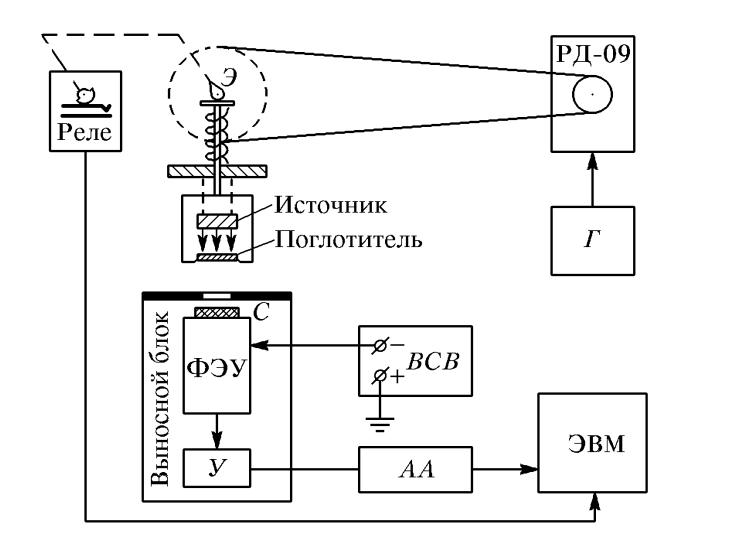
\includegraphics[width = 0.4\textwidth]{experimenta_setup.png}
        \caption{Схема экспериментальной установки.}
        \label{fig:experimental_setup}
    \end{center}
\end{figure}

Схема экспериментальной установки изображена на рисунке $\ref{fig:experimental_setup}$.
Для детектирования $\gamma$ - квантов используется ФЭУ. Пересчетное устройство позволяет
устанавливать верхний и нижний пороги срабатывания. Таким образом, налетающие $\gamma$ - кванты
могут быть отсортированы по энергии(проанализирован спектр источника).

Поглотитель $\gamma$ - излучения приводится в движение посредством механизма преобразования
вращательного движения в поступательное. <<Источником>> вращательного движения является
электронный двигатель РД-09.






\section*{\textcolor{header}{Обработка экспериментальных данных}}

\begin{figure}[hbtp]
    \begin{center}
        % This file was created with tikzplotlib v0.10.1.
\begin{tikzpicture}

\definecolor{darkgray176}{RGB}{176,176,176}
\definecolor{steelblue31119180}{RGB}{31,119,180}

\begin{groupplot}[group style={group size=1 by 3}]
\nextgroupplot[
tick align=outside,
tick pos=left,
x grid style={darkgray176},
xmin=-0.055, xmax=0.055,
xtick style={color=black},
y grid style={darkgray176},
ymin=-0.055, ymax=0.055,
ytick style={color=black}
]
\addplot [draw=none, draw=steelblue31119180, fill=steelblue31119180, mark=*]
table{%
x  y
0 -0.5
0.13260155 -0.5
0.259789935392427 -0.447316845794121
0.353553390593274 -0.353553390593274
0.447316845794121 -0.259789935392427
0.5 -0.13260155
0.5 0
0.5 0.13260155
0.447316845794121 0.259789935392427
0.353553390593274 0.353553390593274
0.259789935392427 0.447316845794121
0.13260155 0.5
0 0.5
-0.13260155 0.5
-0.259789935392427 0.447316845794121
-0.353553390593274 0.353553390593274
-0.447316845794121 0.259789935392427
-0.5 0.13260155
-0.5 0
-0.5 -0.13260155
-0.447316845794121 -0.259789935392427
-0.353553390593274 -0.353553390593274
-0.259789935392427 -0.447316845794121
-0.13260155 -0.5
0 -0.5
0 -0.5
};

\nextgroupplot[
tick align=outside,
tick pos=left,
x grid style={darkgray176},
xmin=-3.5365, xmax=4.0865,
xtick style={color=black},
y grid style={darkgray176},
ymin=787.03, ymax=907.37,
ytick style={color=black}
]
\addplot [draw=steelblue31119180, fill=steelblue31119180, mark=*, only marks]
table{%
x  y
-3.19 898.9
-2.94 883.7
-2.42 884.2
-2.04 894.2
-1.56 888.4
-1.69 897.5
-1.54 901.9
-1.38 891.8
-1.08 893.2
-0.78 882.7
3.74 857.2
3.21 852.7
2.94 848
2.44 792.5
2.07 801.8
1.6 868.5
1.73 852.1
1.56 870.7
1.39 880.3
1.09 880.7
0.79 898
};

\nextgroupplot[
tick align=outside,
tick pos=left,
x grid style={darkgray176},
xmin=-0.055, xmax=0.055,
xtick style={color=black},
y grid style={darkgray176},
ymin=-0.055, ymax=0.055,
ytick style={color=black}
]
\addplot [draw=none, draw=steelblue31119180, fill=steelblue31119180, mark=*]
table{%
x  y
0 -0.5
0.13260155 -0.5
0.259789935392427 -0.447316845794121
0.353553390593274 -0.353553390593274
0.447316845794121 -0.259789935392427
0.5 -0.13260155
0.5 0
0.5 0.13260155
0.447316845794121 0.259789935392427
0.353553390593274 0.353553390593274
0.259789935392427 0.447316845794121
0.13260155 0.5
0 0.5
-0.13260155 0.5
-0.259789935392427 0.447316845794121
-0.353553390593274 0.353553390593274
-0.447316845794121 0.259789935392427
-0.5 0.13260155
-0.5 0
-0.5 -0.13260155
-0.447316845794121 -0.259789935392427
-0.353553390593274 -0.353553390593274
-0.259789935392427 -0.447316845794121
-0.13260155 -0.5
0 -0.5
0 -0.5
};
\end{groupplot}

\end{tikzpicture}

    \end{center}
    \caption{Экспериментальные точки, приближенные контуром Воигта( смотрите формулу $\ref{approximation_fucntion_1}$)}.
    \label{fig:raw_data}
\end{figure}

Для предварительных выводов приблизим данные контуром Воигта, часто
используемом в спектроскопии.

\begin{equation}
    \begin{aligned}
        f(x) = O - A \cdot V(x + B, \sigma, \gamma) \text{ ,} \\
        \text{ где } V(x, \sigma, \gamma) = \int_{- \infty}^{\infty} G(x', \sigma) L(x - x', \gamma) dx'
    \end{aligned}
    \label{approximation_fucntion_1}
\end{equation}

Функция $V(x, \sigma, \gamma)$ - свёртка плотностей <<центрированных>> нормального распределения и распределения Коши.
Параметр $\sigma$ - дисперсия нормального распределения, $\gamma$ - коэффициент масштаба распределения Коши.

Другими словами, величины $\sigma$ и $\gamma$ показывают степень родства искомого профиля с естественным и Лоренцевским профилем.
Как видно на рисунке $\ref{fig:raw_data}$, параметр $\gamma$ всегда больше параметра $\sigma$. ДОБАВИТЬ ВЫВОД ИЗ ЭТОГО
\begin{figure}[hbtp]
    % This file was created with tikzplotlib v0.10.1.
\begin{tikzpicture}

\definecolor{darkgray176}{RGB}{176,176,176}
\definecolor{indianred2178379}{RGB}{217,83,79}
\definecolor{lightgray204}{RGB}{204,204,204}
\definecolor{mediumturquoise91192222}{RGB}{91,192,222}

\begin{groupplot}[group style={group size=2 by 1}]
\nextgroupplot[
height=8cm,
legend cell align={left},
legend style={
  fill opacity=0.8,
  draw opacity=1,
  text opacity=1,
  at={(0.03,0.97)},
  anchor=north west,
  draw=lightgray204
},
minor xtick={},
minor ytick={},
tick align=outside,
tick pos=left,
title={Толщина поглотителя 180 микрон},
width=9cm,
x grid style={darkgray176},
xmajorgrids,
xmin=-2, xmax=3.2,
xtick style={color=black},
xtick={-2,-1,0,1,2,3,4},
y grid style={darkgray176},
ymajorgrids,
ymin=0, ymax=0.6,
ytick style={color=black},
ytick={0,0.05,0.1,0.15,0.2,0.25,0.3,0.35,0.4,0.45,0.5,0.55,0.6,0.65,0.7,0.75,0.8,0.85,0.9,0.95}
]
\draw[draw=none,fill=mediumturquoise91192222,fill opacity=0.8] (axis cs:-3.18927610797183,0) rectangle (axis cs:-3.15459555245486,0.0484421306105659);
\draw[draw=none,fill=mediumturquoise91192222,fill opacity=0.8] (axis cs:-3.15459555245486,0) rectangle (axis cs:-3.11991499693789,0.04382859436194);
\draw[draw=none,fill=mediumturquoise91192222,fill opacity=0.8] (axis cs:-3.11991499693789,0) rectangle (axis cs:-3.08523444142092,0.0570925110767384);
\draw[draw=none,fill=mediumturquoise91192222,fill opacity=0.8] (axis cs:-3.08523444142092,0) rectangle (axis cs:-3.05055388590395,0.0409451342065492);
\draw[draw=none,fill=mediumturquoise91192222,fill opacity=0.8] (axis cs:-3.05055388590395,0) rectangle (axis cs:-3.01587333038698,0.0530556668591912);
\draw[draw=none,fill=mediumturquoise91192222,fill opacity=0.8] (axis cs:-3.01587333038698,0) rectangle (axis cs:-2.98119277487001,0.0415218262376274);
\draw[draw=none,fill=mediumturquoise91192222,fill opacity=0.8] (axis cs:-2.98119277487001,0) rectangle (axis cs:-2.94651221935304,0.0570925110767384);
\draw[draw=none,fill=mediumturquoise91192222,fill opacity=0.8] (axis cs:-2.94651221935304,0) rectangle (axis cs:-2.91183166383607,0.0490188226416434);
\draw[draw=none,fill=mediumturquoise91192222,fill opacity=0.8] (axis cs:-2.91183166383607,0) rectangle (axis cs:-2.8771511083191,0.066319583573989);
\draw[draw=none,fill=mediumturquoise91192222,fill opacity=0.8] (axis cs:-2.8771511083191,0) rectangle (axis cs:-2.84247055280214,0.0588225871699729);
\draw[draw=none,fill=mediumturquoise91192222,fill opacity=0.8] (axis cs:-2.84247055280214,0) rectangle (axis cs:-2.80778999728517,0.058245895138894);
\draw[draw=none,fill=mediumturquoise91192222,fill opacity=0.8] (axis cs:-2.80778999728517,0) rectangle (axis cs:-2.7731094417682,0.0507488987348785);
\draw[draw=none,fill=mediumturquoise91192222,fill opacity=0.8] (axis cs:-2.7731094417682,0) rectangle (axis cs:-2.73842888625123,0.0449819784240963);
\draw[draw=none,fill=mediumturquoise91192222,fill opacity=0.8] (axis cs:-2.73842888625123,0) rectangle (axis cs:-2.70374833073426,0.059399279201051);
\draw[draw=none,fill=mediumturquoise91192222,fill opacity=0.8] (axis cs:-2.70374833073426,0) rectangle (axis cs:-2.66906777521729,0.0547857429524257);
\draw[draw=none,fill=mediumturquoise91192222,fill opacity=0.8] (axis cs:-2.66906777521729,0) rectangle (axis cs:-2.63438721970032,0.0426752102997837);
\draw[draw=none,fill=mediumturquoise91192222,fill opacity=0.8] (axis cs:-2.63438721970032,0) rectangle (axis cs:-2.59970666418335,0.0472887465484089);
\draw[draw=none,fill=mediumturquoise91192222,fill opacity=0.8] (axis cs:-2.59970666418335,0) rectangle (axis cs:-2.56502610866638,0.052478974828113);
\draw[draw=none,fill=mediumturquoise91192222,fill opacity=0.8] (axis cs:-2.56502610866638,0) rectangle (axis cs:-2.53034555314941,0.0478654385794877);
\draw[draw=none,fill=mediumturquoise91192222,fill opacity=0.8] (axis cs:-2.53034555314941,0) rectangle (axis cs:-2.49566499763244,0.0519022827970342);
\draw[draw=none,fill=mediumturquoise91192222,fill opacity=0.8] (axis cs:-2.49566499763244,0) rectangle (axis cs:-2.46098444211547,0.0467120545173314);
\draw[draw=none,fill=mediumturquoise91192222,fill opacity=0.8] (axis cs:-2.46098444211547,0) rectangle (axis cs:-2.4263038865985,0.0478654385794871);
\draw[draw=none,fill=mediumturquoise91192222,fill opacity=0.8] (axis cs:-2.4263038865985,0) rectangle (axis cs:-2.39162333108153,0.0536323588902694);
\draw[draw=none,fill=mediumturquoise91192222,fill opacity=0.8] (axis cs:-2.39162333108153,0) rectangle (axis cs:-2.35694277556456,0.0542090509213475);
\draw[draw=none,fill=mediumturquoise91192222,fill opacity=0.8] (axis cs:-2.35694277556456,0) rectangle (axis cs:-2.3222622200476,0.0576692031078158);
\draw[draw=none,fill=mediumturquoise91192222,fill opacity=0.8] (axis cs:-2.32226222004759,0) rectangle (axis cs:-2.28758166453063,0.0507488987348779);
\draw[draw=none,fill=mediumturquoise91192222,fill opacity=0.8] (axis cs:-2.28758166453063,0) rectangle (axis cs:-2.25290110901366,0.0519022827970349);
\draw[draw=none,fill=mediumturquoise91192222,fill opacity=0.8] (axis cs:-2.25290110901366,0) rectangle (axis cs:-2.21822055349669,0.0484421306105659);
\draw[draw=none,fill=mediumturquoise91192222,fill opacity=0.8] (axis cs:-2.21822055349669,0) rectangle (axis cs:-2.18353999797972,0.049018822641644);
\draw[draw=none,fill=mediumturquoise91192222,fill opacity=0.8] (axis cs:-2.18353999797972,0) rectangle (axis cs:-2.14885944246275,0.051325590765956);
\draw[draw=none,fill=mediumturquoise91192222,fill opacity=0.8] (axis cs:-2.14885944246275,0) rectangle (axis cs:-2.11417888694578,0.0501722067037997);
\draw[draw=none,fill=mediumturquoise91192222,fill opacity=0.8] (axis cs:-2.11417888694578,0) rectangle (axis cs:-2.07949833142881,0.0478654385794877);
\draw[draw=none,fill=mediumturquoise91192222,fill opacity=0.8] (axis cs:-2.07949833142881,0) rectangle (axis cs:-2.04481777591184,0.0495955146727222);
\draw[draw=none,fill=mediumturquoise91192222,fill opacity=0.8] (axis cs:-2.04481777591184,0) rectangle (axis cs:-2.01013722039487,0.0536323588902687);
\draw[draw=none,fill=mediumturquoise91192222,fill opacity=0.8] (axis cs:-2.01013722039487,0) rectangle (axis cs:-1.9754566648779,0.0478654385794874);
\draw[draw=none,fill=mediumturquoise91192222,fill opacity=0.8] (axis cs:-1.9754566648779,0) rectangle (axis cs:-1.94077610936093,0.0478654385794874);
\draw[draw=none,fill=mediumturquoise91192222,fill opacity=0.8] (axis cs:-1.94077610936093,0) rectangle (axis cs:-1.90609555384396,0.0501722067038004);
\draw[draw=none,fill=mediumturquoise91192222,fill opacity=0.8] (axis cs:-1.90609555384396,0) rectangle (axis cs:-1.87141499832699,0.0559391270145817);
\draw[draw=none,fill=mediumturquoise91192222,fill opacity=0.8] (axis cs:-1.87141499832699,0) rectangle (axis cs:-1.83673444281002,0.0634361234185978);
\draw[draw=none,fill=mediumturquoise91192222,fill opacity=0.8] (axis cs:-1.83673444281002,0) rectangle (axis cs:-1.80205388729306,0.0478654385794874);
\draw[draw=none,fill=mediumturquoise91192222,fill opacity=0.8] (axis cs:-1.80205388729305,0) rectangle (axis cs:-1.76737333177609,0.0519022827970345);
\draw[draw=none,fill=mediumturquoise91192222,fill opacity=0.8] (axis cs:-1.76737333177609,0) rectangle (axis cs:-1.73269277625912,0.0478654385794874);
\draw[draw=none,fill=mediumturquoise91192222,fill opacity=0.8] (axis cs:-1.73269277625912,0) rectangle (axis cs:-1.69801222074215,0.0467120545173311);
\draw[draw=none,fill=mediumturquoise91192222,fill opacity=0.8] (axis cs:-1.69801222074215,0) rectangle (axis cs:-1.66333166522518,0.0536323588902694);
\draw[draw=none,fill=mediumturquoise91192222,fill opacity=0.8] (axis cs:-1.66333166522518,0) rectangle (axis cs:-1.62865110970821,0.0467120545173311);
\draw[draw=none,fill=mediumturquoise91192222,fill opacity=0.8] (axis cs:-1.62865110970821,0) rectangle (axis cs:-1.59397055419124,0.0530556668591909);
\draw[draw=none,fill=mediumturquoise91192222,fill opacity=0.8] (axis cs:-1.59397055419124,0) rectangle (axis cs:-1.55928999867427,0.0472887465484092);
\draw[draw=none,fill=mediumturquoise91192222,fill opacity=0.8] (axis cs:-1.55928999867427,0) rectangle (axis cs:-1.5246094431573,0.0513255907659564);
\draw[draw=none,fill=mediumturquoise91192222,fill opacity=0.8] (axis cs:-1.5246094431573,0) rectangle (axis cs:-1.48992888764033,0.0455586704551748);
\draw[draw=none,fill=mediumturquoise91192222,fill opacity=0.8] (axis cs:-1.48992888764033,0) rectangle (axis cs:-1.45524833212336,0.0490188226416437);
\draw[draw=none,fill=mediumturquoise91192222,fill opacity=0.8] (axis cs:-1.45524833212336,0) rectangle (axis cs:-1.42056777660639,0.0472887465484092);
\draw[draw=none,fill=mediumturquoise91192222,fill opacity=0.8] (axis cs:-1.42056777660639,0) rectangle (axis cs:-1.38588722108942,0.0490188226416437);
\draw[draw=none,fill=mediumturquoise91192222,fill opacity=0.8] (axis cs:-1.38588722108942,0) rectangle (axis cs:-1.35120666557245,0.0461353624862532);
\draw[draw=none,fill=mediumturquoise91192222,fill opacity=0.8] (axis cs:-1.35120666557245,0) rectangle (axis cs:-1.31652611005548,0.039215058113315);
\draw[draw=none,fill=mediumturquoise91192222,fill opacity=0.8] (axis cs:-1.31652611005548,0) rectangle (axis cs:-1.28184555453852,0.0611293552942851);
\draw[draw=none,fill=mediumturquoise91192222,fill opacity=0.8] (axis cs:-1.28184555453852,0) rectangle (axis cs:-1.24716499902155,0.0403684421754713);
\draw[draw=none,fill=mediumturquoise91192222,fill opacity=0.8] (axis cs:-1.24716499902155,0) rectangle (axis cs:-1.21248444350458,0.0576692031078162);
\draw[draw=none,fill=mediumturquoise91192222,fill opacity=0.8] (axis cs:-1.21248444350458,0) rectangle (axis cs:-1.17780388798761,0.0553624349835039);
\draw[draw=none,fill=mediumturquoise91192222,fill opacity=0.8] (axis cs:-1.17780388798761,0) rectangle (axis cs:-1.14312333247064,0.0467120545173308);
\draw[draw=none,fill=mediumturquoise91192222,fill opacity=0.8] (axis cs:-1.14312333247064,0) rectangle (axis cs:-1.10844277695367,0.0472887465484096);
\draw[draw=none,fill=mediumturquoise91192222,fill opacity=0.8] (axis cs:-1.10844277695367,0) rectangle (axis cs:-1.0737622214367,0.0599759712321284);
\draw[draw=none,fill=mediumturquoise91192222,fill opacity=0.8] (axis cs:-1.0737622214367,0) rectangle (axis cs:-1.03908166591973,0.0397917501443934);
\draw[draw=none,fill=mediumturquoise91192222,fill opacity=0.8] (axis cs:-1.03908166591973,0) rectangle (axis cs:-1.00440111040276,0.0426752102997837);
\draw[draw=none,fill=mediumturquoise91192222,fill opacity=0.8] (axis cs:-1.00440111040276,0) rectangle (axis cs:-0.969720554885791,0.0444052863930187);
\draw[draw=none,fill=mediumturquoise91192222,fill opacity=0.8] (axis cs:-0.969720554885791,0) rectangle (axis cs:-0.935039999368822,0.0472887465484096);
\draw[draw=none,fill=mediumturquoise91192222,fill opacity=0.8] (axis cs:-0.935039999368822,0) rectangle (axis cs:-0.900359443851853,0.0444052863930182);
\draw[draw=none,fill=mediumturquoise91192222,fill opacity=0.8] (axis cs:-0.900359443851853,0) rectangle (axis cs:-0.865678888334883,0.0472887465484096);
\draw[draw=none,fill=mediumturquoise91192222,fill opacity=0.8] (axis cs:-0.865678888334883,0) rectangle (axis cs:-0.830998332817914,0.0403684421754711);
\draw[draw=none,fill=mediumturquoise91192222,fill opacity=0.8] (axis cs:-0.830998332817914,0) rectangle (axis cs:-0.796317777300945,0.0507488987348785);
\draw[draw=none,fill=mediumturquoise91192222,fill opacity=0.8] (axis cs:-0.796317777300945,0) rectangle (axis cs:-0.761637221783975,0.04382859436194);
\draw[draw=none,fill=mediumturquoise91192222,fill opacity=0.8] (axis cs:-0.761637221783975,0) rectangle (axis cs:-0.726956666267006,0.0420985182687061);
\draw[draw=none,fill=mediumturquoise91192222,fill opacity=0.8] (axis cs:-0.726956666267006,0) rectangle (axis cs:-0.692276110750036,0.0415218262376274);
\draw[draw=none,fill=mediumturquoise91192222,fill opacity=0.8] (axis cs:-0.692276110750036,0) rectangle (axis cs:-0.657595555233067,0.0397917501443934);
\draw[draw=none,fill=mediumturquoise91192222,fill opacity=0.8] (axis cs:-0.657595555233067,0) rectangle (axis cs:-0.622914999716098,0.0363315979579244);
\draw[draw=none,fill=mediumturquoise91192222,fill opacity=0.8] (axis cs:-0.622914999716098,0) rectangle (axis cs:-0.588234444199129,0.0357549059268458);
\draw[draw=none,fill=mediumturquoise91192222,fill opacity=0.8] (axis cs:-0.588234444199129,0) rectangle (axis cs:-0.553553888682159,0.0415218262376279);
\draw[draw=none,fill=mediumturquoise91192222,fill opacity=0.8] (axis cs:-0.553553888682159,0) rectangle (axis cs:-0.51887333316519,0.0426752102997837);
\draw[draw=none,fill=mediumturquoise91192222,fill opacity=0.8] (axis cs:-0.51887333316519,0) rectangle (axis cs:-0.484192777648221,0.0461353624862532);
\draw[draw=none,fill=mediumturquoise91192222,fill opacity=0.8] (axis cs:-0.484192777648221,0) rectangle (axis cs:-0.449512222131251,0.0397917501443929);
\draw[draw=none,fill=mediumturquoise91192222,fill opacity=0.8] (axis cs:-0.449512222131251,0) rectangle (axis cs:-0.414831666614282,0.0547857429524257);
\draw[draw=none,fill=mediumturquoise91192222,fill opacity=0.8] (axis cs:-0.414831666614282,0) rectangle (axis cs:-0.380151111097313,0.0426752102997842);
\draw[draw=none,fill=mediumturquoise91192222,fill opacity=0.8] (axis cs:-0.380151111097313,0) rectangle (axis cs:-0.345470555580343,0.0622827393564411);
\draw[draw=none,fill=mediumturquoise91192222,fill opacity=0.8] (axis cs:-0.345470555580343,0) rectangle (axis cs:-0.310790000063374,0.0438285943619406);
\draw[draw=none,fill=mediumturquoise91192222,fill opacity=0.8] (axis cs:-0.310790000063374,0) rectangle (axis cs:-0.276109444546405,0.0403684421754711);
\draw[draw=none,fill=mediumturquoise91192222,fill opacity=0.8] (axis cs:-0.276109444546405,0) rectangle (axis cs:-0.241428889029435,0.0403684421754716);
\draw[draw=none,fill=mediumturquoise91192222,fill opacity=0.8] (axis cs:-0.241428889029435,0) rectangle (axis cs:-0.206748333512466,0.0495955146727216);
\draw[draw=none,fill=mediumturquoise91192222,fill opacity=0.8] (axis cs:-0.206748333512466,0) rectangle (axis cs:-0.172067777995497,0.0501722067038004);
\draw[draw=none,fill=mediumturquoise91192222,fill opacity=0.8] (axis cs:-0.172067777995497,0) rectangle (axis cs:-0.137387222478528,0.0444052863930187);
\draw[draw=none,fill=mediumturquoise91192222,fill opacity=0.8] (axis cs:-0.137387222478528,0) rectangle (axis cs:-0.102706666961558,0.051325590765956);
\draw[draw=none,fill=mediumturquoise91192222,fill opacity=0.8] (axis cs:-0.102706666961558,0) rectangle (axis cs:-0.0680261114445888,0.0392150581133152);
\draw[draw=none,fill=mediumturquoise91192222,fill opacity=0.8] (axis cs:-0.0680261114445888,0) rectangle (axis cs:-0.0333455559276192,0.0461353624862526);
\draw[draw=none,fill=mediumturquoise91192222,fill opacity=0.8] (axis cs:-0.0333455559276192,0) rectangle (axis cs:0.00133499958934991,0.0553624349835039);
\draw[draw=none,fill=mediumturquoise91192222,fill opacity=0.8] (axis cs:0.00133499958934991,0) rectangle (axis cs:0.0360155551063195,0.0374849820200803);
\draw[draw=none,fill=mediumturquoise91192222,fill opacity=0.8] (axis cs:0.0360155551063195,0) rectangle (axis cs:0.0706961106232886,0.0374849820200807);
\draw[draw=none,fill=mediumturquoise91192222,fill opacity=0.8] (axis cs:0.0706961106232886,0) rectangle (axis cs:0.105376666140258,0.0478654385794871);
\draw[draw=none,fill=mediumturquoise91192222,fill opacity=0.8] (axis cs:0.105376666140258,0) rectangle (axis cs:0.140057221657227,0.0472887465484096);
\draw[draw=none,fill=mediumturquoise91192222,fill opacity=0.8] (axis cs:0.140057221657227,0) rectangle (axis cs:0.174737777174196,0.049018822641644);
\draw[draw=none,fill=mediumturquoise91192222,fill opacity=0.8] (axis cs:0.174737777174196,0) rectangle (axis cs:0.209418332691166,0.0565158190456595);
\draw[draw=none,fill=mediumturquoise91192222,fill opacity=0.8] (axis cs:0.209418332691166,0) rectangle (axis cs:0.244098888208135,0.0444052863930187);
\draw[draw=none,fill=mediumturquoise91192222,fill opacity=0.8] (axis cs:0.244098888208135,0) rectangle (axis cs:0.278779443725105,0.054785742952425);
\draw[draw=none,fill=mediumturquoise91192222,fill opacity=0.8] (axis cs:0.278779443725105,0) rectangle (axis cs:0.313459999242074,0.0380616740511589);
\draw[draw=none,fill=mediumturquoise91192222,fill opacity=0.8] (axis cs:0.313459999242074,0) rectangle (axis cs:0.348140554759043,0.0519022827970342);
\draw[draw=none,fill=mediumturquoise91192222,fill opacity=0.8] (axis cs:0.348140554759043,0) rectangle (axis cs:0.382821110276013,0.0397917501443934);
\draw[draw=none,fill=mediumturquoise91192222,fill opacity=0.8] (axis cs:0.382821110276013,0) rectangle (axis cs:0.417501665792982,0.0397917501443929);
\draw[draw=none,fill=mediumturquoise91192222,fill opacity=0.8] (axis cs:0.417501665792982,0) rectangle (axis cs:0.452182221309951,0.0374849820200807);
\draw[draw=none,fill=mediumturquoise91192222,fill opacity=0.8] (axis cs:0.452182221309951,0) rectangle (axis cs:0.48686277682692,0.0501722067038004);
\draw[draw=none,fill=mediumturquoise91192222,fill opacity=0.8] (axis cs:0.48686277682692,0) rectangle (axis cs:0.52154333234389,0.0415218262376274);
\draw[draw=none,fill=mediumturquoise91192222,fill opacity=0.8] (axis cs:0.52154333234389,0) rectangle (axis cs:0.556223887860859,0.0478654385794877);
\draw[draw=none,fill=mediumturquoise91192222,fill opacity=0.8] (axis cs:0.556223887860859,0) rectangle (axis cs:0.590904443377829,0.0519022827970342);
\draw[draw=none,fill=mediumturquoise91192222,fill opacity=0.8] (axis cs:0.590904443377829,0) rectangle (axis cs:0.625584998894798,0.0484421306105659);
\draw[draw=none,fill=mediumturquoise91192222,fill opacity=0.8] (axis cs:0.625584998894798,0) rectangle (axis cs:0.660265554411767,0.0495955146727216);
\draw[draw=none,fill=mediumturquoise91192222,fill opacity=0.8] (axis cs:0.660265554411767,0) rectangle (axis cs:0.694946109928737,0.0461353624862532);
\draw[draw=none,fill=mediumturquoise91192222,fill opacity=0.8] (axis cs:0.694946109928737,0) rectangle (axis cs:0.729626665445706,0.0576692031078165);
\draw[draw=none,fill=mediumturquoise91192222,fill opacity=0.8] (axis cs:0.729626665445706,0) rectangle (axis cs:0.764307220962675,0.0565158190456595);
\draw[draw=none,fill=mediumturquoise91192222,fill opacity=0.8] (axis cs:0.764307220962675,0) rectangle (axis cs:0.798987776479644,0.0444052863930187);
\draw[draw=none,fill=mediumturquoise91192222,fill opacity=0.8] (axis cs:0.798987776479644,0) rectangle (axis cs:0.833668331996614,0.0484421306105659);
\draw[draw=none,fill=mediumturquoise91192222,fill opacity=0.8] (axis cs:0.833668331996614,0) rectangle (axis cs:0.868348887513584,0.0605526632632058);
\draw[draw=none,fill=mediumturquoise91192222,fill opacity=0.8] (axis cs:0.868348887513584,0) rectangle (axis cs:0.903029443030553,0.0519022827970349);
\draw[draw=none,fill=mediumturquoise91192222,fill opacity=0.8] (axis cs:0.903029443030553,0) rectangle (axis cs:0.937709998547522,0.0622827393564418);
\draw[draw=none,fill=mediumturquoise91192222,fill opacity=0.8] (axis cs:0.937709998547522,0) rectangle (axis cs:0.972390554064491,0.0588225871699729);
\draw[draw=none,fill=mediumturquoise91192222,fill opacity=0.8] (axis cs:0.972390554064491,0) rectangle (axis cs:1.00707110958146,0.0472887465484096);
\draw[draw=none,fill=mediumturquoise91192222,fill opacity=0.8] (axis cs:1.00707110958146,0) rectangle (axis cs:1.04175166509843,0.0692030437293781);
\draw[draw=none,fill=mediumturquoise91192222,fill opacity=0.8] (axis cs:1.04175166509843,0) rectangle (axis cs:1.0764322206154,0.0588225871699729);
\draw[draw=none,fill=mediumturquoise91192222,fill opacity=0.8] (axis cs:1.0764322206154,0) rectangle (axis cs:1.11111277613237,0.0761233481023178);
\draw[draw=none,fill=mediumturquoise91192222,fill opacity=0.8] (axis cs:1.11111277613237,0) rectangle (axis cs:1.14579333164934,0.0542090509213475);
\draw[draw=none,fill=mediumturquoise91192222,fill opacity=0.8] (axis cs:1.14579333164934,0) rectangle (axis cs:1.18047388716631,0.0732398879469251);
\draw[draw=none,fill=mediumturquoise91192222,fill opacity=0.8] (axis cs:1.18047388716631,0) rectangle (axis cs:1.21515444268328,0.073239887946927);
\draw[draw=none,fill=mediumturquoise91192222,fill opacity=0.8] (axis cs:1.21515444268328,0) rectangle (axis cs:1.24983499820025,0.083620344506334);
\draw[draw=none,fill=mediumturquoise91192222,fill opacity=0.8] (axis cs:1.24983499820025,0) rectangle (axis cs:1.28451555371722,0.069779735760458);
\draw[draw=none,fill=mediumturquoise91192222,fill opacity=0.8] (axis cs:1.28451555371722,0) rectangle (axis cs:1.31919610923418,0.0818902684130995);
\draw[draw=none,fill=mediumturquoise91192222,fill opacity=0.8] (axis cs:1.31919610923418,0) rectangle (axis cs:1.35387666475115,0.107841409811614);
\draw[draw=none,fill=mediumturquoise91192222,fill opacity=0.8] (axis cs:1.35387666475115,0) rectangle (axis cs:1.38855722026812,0.0940008010657409);
\draw[draw=none,fill=mediumturquoise91192222,fill opacity=0.8] (axis cs:1.38855722026812,0) rectangle (axis cs:1.42323777578509,0.109571485904851);
\draw[draw=none,fill=mediumturquoise91192222,fill opacity=0.8] (axis cs:1.42323777578509,0) rectangle (axis cs:1.45791833130206,0.115915098246711);
\draw[draw=none,fill=mediumturquoise91192222,fill opacity=0.8] (axis cs:1.45791833130206,0) rectangle (axis cs:1.49259888681903,0.138982779489834);
\draw[draw=none,fill=mediumturquoise91192222,fill opacity=0.8] (axis cs:1.49259888681903,0) rectangle (axis cs:1.527279442336,0.134945935272291);
\draw[draw=none,fill=mediumturquoise91192222,fill opacity=0.8] (axis cs:1.527279442336,0) rectangle (axis cs:1.56195999785297,0.155706848391105);
\draw[draw=none,fill=mediumturquoise91192222,fill opacity=0.8] (axis cs:1.56195999785297,0) rectangle (axis cs:1.59664055336994,0.168970765105902);
\draw[draw=none,fill=mediumturquoise91192222,fill opacity=0.8] (axis cs:1.59664055336994,0) rectangle (axis cs:1.63132110888691,0.179927913696388);
\draw[draw=none,fill=mediumturquoise91192222,fill opacity=0.8] (axis cs:1.63132110888691,0) rectangle (axis cs:1.66600166440388,0.20876251525029);
\draw[draw=none,fill=mediumturquoise91192222,fill opacity=0.8] (axis cs:1.66600166440388,0) rectangle (axis cs:1.70068221992085,0.217412895716468);
\draw[draw=none,fill=mediumturquoise91192222,fill opacity=0.8] (axis cs:1.70068221992085,0) rectangle (axis cs:1.73536277543782,0.245670805239298);
\draw[draw=none,fill=mediumturquoise91192222,fill opacity=0.8] (axis cs:1.73536277543782,0) rectangle (axis cs:1.77004333095479,0.255474569767627);
\draw[draw=none,fill=mediumturquoise91192222,fill opacity=0.8] (axis cs:1.77004333095479,0) rectangle (axis cs:1.80472388647176,0.263548258202715);
\draw[draw=none,fill=mediumturquoise91192222,fill opacity=0.8] (axis cs:1.80472388647176,0) rectangle (axis cs:1.83940444198872,0.295843011943099);
\draw[draw=none,fill=mediumturquoise91192222,fill opacity=0.8] (axis cs:1.83940444198872,0) rectangle (axis cs:1.87408499750569,0.304493392409271);
\draw[draw=none,fill=mediumturquoise91192222,fill opacity=0.8] (axis cs:1.87408499750569,0) rectangle (axis cs:1.90876555302266,0.354088907081993);
\draw[draw=none,fill=mediumturquoise91192222,fill opacity=0.8] (axis cs:1.90876555302266,0) rectangle (axis cs:1.94344610853963,0.371966360045417);
\draw[draw=none,fill=mediumturquoise91192222,fill opacity=0.8] (axis cs:1.94344610853963,0) rectangle (axis cs:1.9781266640566,0.386960352853439);
\draw[draw=none,fill=mediumturquoise91192222,fill opacity=0.8] (axis cs:1.9781266640566,0) rectangle (axis cs:2.01280721957357,0.416948338469513);
\draw[draw=none,fill=mediumturquoise91192222,fill opacity=0.8] (axis cs:2.01280721957357,0) rectangle (axis cs:2.04748777509054,0.419255106593826);
\draw[draw=none,fill=mediumturquoise91192222,fill opacity=0.8] (axis cs:2.04748777509054,0) rectangle (axis cs:2.08216833060751,0.432519023308624);
\draw[draw=none,fill=mediumturquoise91192222,fill opacity=0.8] (axis cs:2.08216833060751,0) rectangle (axis cs:2.11684888612448,0.474040849546252);
\draw[draw=none,fill=mediumturquoise91192222,fill opacity=0.8] (axis cs:2.11684888612448,0) rectangle (axis cs:2.15152944164145,0.490764918447506);
\draw[draw=none,fill=mediumturquoise91192222,fill opacity=0.8] (axis cs:2.15152944164145,0) rectangle (axis cs:2.18620999715842,0.525943132343287);
\draw[draw=none,fill=mediumturquoise91192222,fill opacity=0.8] (axis cs:2.18620999715842,0) rectangle (axis cs:2.22089055267539,0.519599520001427);
\draw[draw=none,fill=mediumturquoise91192222,fill opacity=0.8] (axis cs:2.22089055267539,0) rectangle (axis cs:2.25557110819236,0.526519824374365);
\draw[draw=none,fill=mediumturquoise91192222,fill opacity=0.8] (axis cs:2.25557110819236,0) rectangle (axis cs:2.29025166370933,0.512102523597398);
\draw[draw=none,fill=mediumturquoise91192222,fill opacity=0.8] (axis cs:2.29025166370933,0) rectangle (axis cs:2.3249322192263,0.546127353431022);
\draw[draw=none,fill=mediumturquoise91192222,fill opacity=0.8] (axis cs:2.3249322192263,0) rectangle (axis cs:2.35961277474326,0.540937125151319);
\draw[draw=none,fill=mediumturquoise91192222,fill opacity=0.8] (axis cs:2.35961277474326,0) rectangle (axis cs:2.39429333026023,0.558237886083664);
\draw[draw=none,fill=mediumturquoise91192222,fill opacity=0.8] (axis cs:2.39429333026023,0) rectangle (axis cs:2.4289738857772,0.554777733897195);
\draw[draw=none,fill=mediumturquoise91192222,fill opacity=0.8] (axis cs:2.4289738857772,0) rectangle (axis cs:2.46365444129417,0.544397277337774);
\draw[draw=none,fill=mediumturquoise91192222,fill opacity=0.8] (axis cs:2.46365444129417,0) rectangle (axis cs:2.49833499681114,0.526519824374365);
\draw[draw=none,fill=mediumturquoise91192222,fill opacity=0.8] (axis cs:2.49833499681114,0) rectangle (axis cs:2.53301555232811,0.523059672187896);
\draw[draw=none,fill=mediumturquoise91192222,fill opacity=0.8] (axis cs:2.53301555232811,0) rectangle (axis cs:2.56769610784508,0.492494994540753);
\draw[draw=none,fill=mediumturquoise91192222,fill opacity=0.8] (axis cs:2.56769610784508,0) rectangle (axis cs:2.60237666336205,0.493071686571819);
\draw[draw=none,fill=mediumturquoise91192222,fill opacity=0.8] (axis cs:2.60237666336205,0) rectangle (axis cs:2.63705721887902,0.459046856738219);
\draw[draw=none,fill=mediumturquoise91192222,fill opacity=0.8] (axis cs:2.63705721887902,0) rectangle (axis cs:2.67173777439599,0.429058871122155);
\draw[draw=none,fill=mediumturquoise91192222,fill opacity=0.8] (axis cs:2.67173777439599,0) rectangle (axis cs:2.70641832991296,0.428482179091077);
\draw[draw=none,fill=mediumturquoise91192222,fill opacity=0.8] (axis cs:2.70641832991296,0) rectangle (axis cs:2.74109888542993,0.388113736915605);
\draw[draw=none,fill=mediumturquoise91192222,fill opacity=0.8] (axis cs:2.74109888542993,0) rectangle (axis cs:2.7757794409469,0.346591910677968);
\draw[draw=none,fill=mediumturquoise91192222,fill opacity=0.8] (axis cs:2.7757794409469,0) rectangle (axis cs:2.81045999646387,0.36158590348601);
\draw[draw=none,fill=mediumturquoise91192222,fill opacity=0.8] (axis cs:2.81045999646387,0) rectangle (axis cs:2.84514055198084,0.343131758491508);
\draw[draw=none,fill=mediumturquoise91192222,fill opacity=0.8] (axis cs:2.84514055198084,0) rectangle (axis cs:2.8798211074978,0.304493392409271);
\draw[draw=none,fill=mediumturquoise91192222,fill opacity=0.8] (axis cs:2.8798211074978,0) rectangle (axis cs:2.91450166301477,0.278542251010754);
\draw[draw=none,fill=mediumturquoise91192222,fill opacity=0.8] (axis cs:2.91450166301477,0) rectangle (axis cs:2.94918221853174,0.280272327103981);
\draw[draw=none,fill=mediumturquoise91192222,fill opacity=0.8] (axis cs:2.94918221853174,0) rectangle (axis cs:2.98386277404871,0.242210653052829);
\draw[draw=none,fill=mediumturquoise91192222,fill opacity=0.8] (axis cs:2.98386277404871,0) rectangle (axis cs:3.01854332956568,0.254321185705471);
\draw[draw=none,fill=mediumturquoise91192222,fill opacity=0.8] (axis cs:3.01854332956568,0) rectangle (axis cs:3.05322388508265,0.227793352275875);
\draw[draw=none,fill=mediumturquoise91192222,fill opacity=0.8] (axis cs:3.05322388508265,0) rectangle (axis cs:3.08790444059962,0.246824189301448);
\draw[draw=none,fill=mediumturquoise91192222,fill opacity=0.8] (axis cs:3.08790444059962,0) rectangle (axis cs:3.12258499611659,0.222603123996172);
\draw[draw=none,fill=mediumturquoise91192222,fill opacity=0.8] (axis cs:3.12258499611659,0) rectangle (axis cs:3.15726555163356,0.239903884928517);
\draw[draw=none,fill=mediumturquoise91192222,fill opacity=0.8] (axis cs:3.15726555163356,0) rectangle (axis cs:3.19194610715053,0.219142971809703);
\draw[draw=none,fill=mediumturquoise91192222,fill opacity=0.8] (axis cs:3.19194610715053,0) rectangle (axis cs:3.2266266626675,0.224333200089406);
\draw[draw=none,fill=mediumturquoise91192222,fill opacity=0.8] (axis cs:3.2266266626675,0) rectangle (axis cs:3.26130721818447,0.217989587747541);
\draw[draw=none,fill=mediumturquoise91192222,fill opacity=0.8] (axis cs:3.26130721818447,0) rectangle (axis cs:3.29598777370144,0.243364037114986);
\draw[draw=none,fill=mediumturquoise91192222,fill opacity=0.8] (axis cs:3.29598777370144,0) rectangle (axis cs:3.33066832921841,0.225486584151563);
\draw[draw=none,fill=mediumturquoise91192222,fill opacity=0.8] (axis cs:3.33066832921841,0) rectangle (axis cs:3.36534888473537,0.242787345083908);
\draw[draw=none,fill=mediumturquoise91192222,fill opacity=0.8] (axis cs:3.36534888473537,0) rectangle (axis cs:3.40002944025234,0.256051261798699);
\draw[draw=none,fill=mediumturquoise91192222,fill opacity=0.8] (axis cs:3.40002944025234,0) rectangle (axis cs:3.43470999576931,0.262394874140565);
\draw[draw=none,fill=mediumturquoise91192222,fill opacity=0.8] (axis cs:3.43470999576931,0) rectangle (axis cs:3.46939055128628,0.24509411320822);
\draw[draw=none,fill=mediumturquoise91192222,fill opacity=0.8] (axis cs:3.46939055128628,0) rectangle (axis cs:3.50407110680325,0.241633961021751);
\draw[draw=none,fill=mediumturquoise91192222,fill opacity=0.8] (axis cs:3.50407110680325,0) rectangle (axis cs:3.53875166232022,0.247400881332533);
\draw[draw=none,fill=mediumturquoise91192222,fill opacity=0.8] (axis cs:3.53875166232022,0) rectangle (axis cs:3.57343221783719,0.250284341487917);
\draw[draw=none,fill=mediumturquoise91192222,fill opacity=0.8] (axis cs:3.57343221783719,0) rectangle (axis cs:3.60811277335416,0.247400881332533);
\draw[draw=none,fill=mediumturquoise91192222,fill opacity=0.8] (axis cs:3.60811277335416,0) rectangle (axis cs:3.64279332887113,0.242210653052829);
\draw[draw=none,fill=mediumturquoise91192222,fill opacity=0.8] (axis cs:3.64279332887113,0) rectangle (axis cs:3.6774738843881,0.231830196493422);
\draw[draw=none,fill=mediumturquoise91192222,fill opacity=0.8] (axis cs:3.6774738843881,0) rectangle (axis cs:3.71215443990507,0.231830196493416);
\draw[draw=none,fill=mediumturquoise91192222,fill opacity=0.8] (axis cs:3.71215443990507,0) rectangle (axis cs:3.74683499542204,0.21683620368539);
\addplot [thick, indianred2178379]
table {%
-3.19 0.00574748534802052
-3.18306306306306 0.00576173556424325
-3.17612612612613 0.00577603866148774
-3.16918918918919 0.00579039490081385
-3.16225225225225 0.00580480454488867
-3.15531531531532 0.00581926785799842
-3.14837837837838 0.00583378510606036
-3.14144144144144 0.00584835655663486
-3.1345045045045 0.00586298247893755
-3.12756756756757 0.00587766314385157
-3.12063063063063 0.00589239882393995
-3.11369369369369 0.00590718979345806
-3.10675675675676 0.00592203632836622
-3.09981981981982 0.00593693870634233
-3.09288288288288 0.00595189720679475
-3.08594594594595 0.00596691211087514
-3.07900900900901 0.0059819837014915
-3.07207207207207 0.00599711226332132
-3.06513513513514 0.00601229808282481
-3.0581981981982 0.00602754144825825
-3.05126126126126 0.00604284264968753
-3.04432432432432 0.00605820197900165
-3.03738738738739 0.00607361972992653
-3.03045045045045 0.0060890961980388
-3.02351351351351 0.00610463168077975
-3.01657657657658 0.00612022647746945
-3.00963963963964 0.0061358808893209
-3.0027027027027 0.00615159521945442
-2.99576576576577 0.00616736977291204
-2.98882882882883 0.00618320485667214
-2.98189189189189 0.00619910077966412
-2.97495495495495 0.00621505785278326
-2.96801801801802 0.0062310763889057
-2.96108108108108 0.00624715670290353
-2.95414414414414 0.00626329911166003
-2.94720720720721 0.00627950393408505
-2.94027027027027 0.00629577149113052
-2.93333333333333 0.00631210210580611
-2.9263963963964 0.00632849610319499
-2.91945945945946 0.0063449538104698
-2.91252252252252 0.00636147555690869
-2.90558558558559 0.00637806167391154
-2.89864864864865 0.00639471249501635
-2.89171171171171 0.0064114283559157
-2.88477477477477 0.00642820959447345
-2.87783783783784 0.00644505655074153
-2.8709009009009 0.00646196956697691
-2.86396396396396 0.00647894898765865
-2.85702702702703 0.00649599515950528
-2.85009009009009 0.0065131084314921
-2.84315315315315 0.00653028915486883
-2.83621621621622 0.00654753768317736
-2.82927927927928 0.00656485437226957
-2.82234234234234 0.00658223958032547
-2.81540540540541 0.0065996936678714
-2.80846846846847 0.00661721699779841
-2.80153153153153 0.00663480993538082
-2.79459459459459 0.00665247284829497
-2.78765765765766 0.00667020610663811
-2.78072072072072 0.00668801008294747
-2.77378378378378 0.00670588515221947
-2.76684684684685 0.00672383169192925
-2.75990990990991 0.00674185008205016
-2.75297297297297 0.00675994070507359
-2.74603603603604 0.00677810394602894
-2.7390990990991 0.00679634019250378
-2.73216216216216 0.00681464983466414
-2.72522522522523 0.00683303326527508
-2.71828828828829 0.00685149087972139
-2.71135135135135 0.00687002307602848
-2.70441441441441 0.0068886302548835
-2.69747747747748 0.00690731281965661
-2.69054054054054 0.00692607117642252
-2.6836036036036 0.00694490573398214
-2.67666666666667 0.00696381690388449
-2.66972972972973 0.00698280510044879
-2.66279279279279 0.00700187074078681
-2.65585585585586 0.00702101424482534
-2.64891891891892 0.00704023603532893
-2.64198198198198 0.00705953653792285
-2.63504504504504 0.00707891618111621
-2.62810810810811 0.00709837539632539
-2.62117117117117 0.00711791461789758
-2.61423423423423 0.00713753428313461
-2.6072972972973 0.00715723483231703
-2.60036036036036 0.00717701670872836
-2.59342342342342 0.00719688035867953
-2.58648648648649 0.00721682623153373
-2.57954954954955 0.00723685477973127
-2.57261261261261 0.00725696645881487
-2.56567567567568 0.00727716172745502
-2.55873873873874 0.00729744104747573
-2.5518018018018 0.00731780488388047
-2.54486486486486 0.00733825370487829
-2.53792792792793 0.00735878798191032
-2.53099099099099 0.0073794081896764
-2.52405405405405 0.00740011480616206
-2.51711711711712 0.0074209083126657
-2.51018018018018 0.00744178919382606
-2.50324324324324 0.00746275793764994
-2.49630630630631 0.0074838150355402
-2.48936936936937 0.00750496098232404
-2.48243243243243 0.0075261962762815
-2.4754954954955 0.0075475214191743
-2.46855855855856 0.00756893691627495
-2.46162162162162 0.00759044327639608
-2.45468468468468 0.00761204101192017
-2.44774774774775 0.00763373063882941
-2.44081081081081 0.00765551267673606
-2.43387387387387 0.00767738764891287
-2.42693693693694 0.00769935608232401
-2.42 0.00772141850765615
-2.41306306306306 0.00774357545934995
-2.40612612612613 0.00776582747563178
-2.39918918918919 0.0077881750985458
-2.39225225225225 0.00781061887398635
-2.38531531531532 0.00783315935173063
-2.37837837837838 0.00785579708547176
-2.37144144144144 0.00787853263285206
-2.3645045045045 0.00790136655549684
-2.35756756756757 0.0079242994190483
-2.35063063063063 0.00794733179319996
-2.34369369369369 0.00797046425173131
-2.33675675675676 0.00799369737254289
-2.32981981981982 0.00801703173769163
-2.32288288288288 0.00804046793342664
-2.31594594594595 0.00806400655022525
-2.30900900900901 0.00808764818282953
-2.30207207207207 0.00811139343028308
-2.29513513513514 0.00813524289596823
-2.2881981981982 0.00815919718764362
-2.28126126126126 0.00818325691748212
-2.27432432432432 0.00820742270210919
-2.26738738738739 0.00823169516264158
-2.26045045045045 0.00825607492472641
-2.25351351351351 0.00828056261858074
-2.24657657657658 0.0083051588790314
-2.23963963963964 0.00832986434555535
-2.2327027027027 0.00835467966232035
-2.22576576576577 0.00837960547822615
-2.21882882882883 0.00840464244694596
-2.21189189189189 0.00842979122696851
-2.20495495495495 0.0084550524816404
-2.19801801801802 0.00848042687920894
-2.19108108108108 0.00850591509286545
-2.18414414414414 0.00853151780078893
-2.17720720720721 0.00855723568619031
-2.17027027027027 0.00858306943735698
-2.16333333333333 0.00860901974769795
-2.1563963963964 0.00863508731578933
-2.14945945945946 0.00866127284542043
-2.14252252252252 0.00868757704564017
-2.13558558558559 0.0087140006308041
-2.12864864864865 0.00874054432062185
-2.12171171171171 0.00876720884020513
-2.11477477477477 0.0087939949201161
-2.10783783783784 0.00882090329641641
-2.1009009009009 0.00884793471071664
-2.09396396396396 0.00887508991022626
-2.08702702702703 0.0089023696478042
-2.08009009009009 0.00892977468200985
-2.07315315315315 0.00895730577715465
-2.06621621621622 0.00898496370335419
-2.05927927927928 0.0090127492365809
-2.05234234234234 0.00904066315871727
-2.04540540540541 0.00906870625760962
-2.03846846846847 0.00909687932712245
-2.03153153153153 0.00912518316719337
-2.02459459459459 0.00915361858388864
-2.01765765765766 0.00918218638945921
-2.01072072072072 0.00921088740239746
-2.00378378378378 0.00923972244749449
-1.99684684684685 0.00926869235589801
-1.98990990990991 0.0092977979651709
-1.98297297297297 0.00932704011935032
-1.97603603603604 0.00935641966900752
-1.9690990990991 0.00938593747130828
-1.96216216216216 0.00941559439007397
-1.95522522522523 0.00944539129584329
-1.94828828828829 0.00947532906593465
-1.94135135135135 0.00950540858450925
-1.93441441441441 0.00953563074263486
-1.92747747747748 0.00956599643835023
-1.92054054054054 0.00959650657673021
-1.9136036036036 0.00962716206995165
-1.90666666666667 0.00965796383735993
-1.89972972972973 0.00968891280553627
-1.89279279279279 0.00972000990836567
-1.88585585585586 0.00975125608710579
-1.87891891891892 0.00978265229045638
-1.87198198198198 0.00981419947462958
-1.86504504504505 0.00984589860342095
-1.85810810810811 0.00987775064828133
-1.85117117117117 0.00990975658838939
-1.84423423423423 0.00994191741072511
-1.8372972972973 0.00997423411014396
-1.83036036036036 0.0100067076894519
-1.82342342342342 0.0100393391594815
-1.81648648648649 0.0100721295391682
-1.80954954954955 0.0101050798556282
-1.80261261261261 0.010138191144237
-1.79567567567568 0.0101714644487082
-1.78873873873874 0.0102049008211743
-1.7818018018018 0.0102385013222672
-1.77486486486486 0.0102722670212006
-1.76792792792793 0.0103061989958528
-1.76099099099099 0.0103402983328503
-1.75405405405405 0.0103745661276528
-1.74711711711712 0.0104090034846389
-1.74018018018018 0.0104436115171927
-1.73324324324324 0.0104783913477917
-1.72630630630631 0.0105133441080949
-1.71936936936937 0.0105484709390332
-1.71243243243243 0.0105837729908995
-1.7054954954955 0.0106192514234406
-1.69855855855856 0.01065490740595
-1.69162162162162 0.0106907421173617
-1.68468468468468 0.0107267567463449
-1.67774774774775 0.0107629524914001
-1.67081081081081 0.0107993305609561
-1.66387387387387 0.0108358921734682
-1.65693693693694 0.0108726385575176
-1.65 0.0109095709519114
-1.64306306306306 0.0109466906057846
-1.63612612612613 0.0109839987787028
-1.62918918918919 0.011021496740766
-1.62225225225225 0.0110591857727137
-1.61531531531532 0.0110970671660314
-1.60837837837838 0.0111351422230582
-1.60144144144144 0.0111734122570956
-1.5945045045045 0.0112118785925174
-1.58756756756757 0.0112505425648814
-1.58063063063063 0.0112894055210419
-1.57369369369369 0.0113284688192638
-1.56675675675676 0.0113677338293378
-1.55981981981982 0.0114072019326972
-1.55288288288288 0.011446874522536
-1.54594594594595 0.011486753003928
-1.53900900900901 0.0115268387939484
-1.53207207207207 0.0115671333217951
-1.52513513513514 0.0116076380289133
-1.5181981981982 0.0116483543691199
-1.51126126126126 0.011689283808731
-1.50432432432432 0.0117304278266894
-1.49738738738739 0.0117717879146944
-1.49045045045045 0.0118133655773335
-1.48351351351351 0.0118551623322147
-1.47657657657658 0.0118971797101009
-1.46963963963964 0.0119394192550464
-1.4627027027027 0.0119818825245339
-1.45576576576577 0.0120245710896142
-1.44882882882883 0.012067486535047
-1.44189189189189 0.0121106304594435
-1.43495495495495 0.0121540044754108
-1.42801801801802 0.0121976102096983
-1.42108108108108 0.012241449303345
-1.41414414414414 0.0122855234118297
-1.40720720720721 0.0123298342052222
-1.40027027027027 0.0123743833683367
-1.39333333333333 0.0124191726008871
-1.3863963963964 0.0124642036176439
-1.37945945945946 0.0125094781485933
-1.37252252252252 0.0125549979390983
-1.36558558558559 0.0126007647500613
-1.35864864864865 0.0126467803580894
-1.35171171171171 0.012693046555661
-1.34477477477477 0.012739565151295
-1.33783783783784 0.0127863379697219
-1.3309009009009 0.012833366852057
-1.32396396396396 0.0128806536559756
-1.31702702702703 0.0129282002558909
-1.31009009009009 0.0129760085431331
-1.30315315315315 0.013024080426132
-1.29621621621622 0.0130724178306009
-1.28927927927928 0.0131210226997231
-1.28234234234234 0.013169896994341
-1.27540540540541 0.013219042693147
-1.26846846846847 0.0132684617928774
-1.26153153153153 0.0133181563085083
-1.25459459459459 0.0133681282734541
-1.24765765765766 0.0134183797397687
-1.24072072072072 0.0134689127783487
-1.23378378378378 0.0135197294791401
-1.22684684684685 0.0135708319513463
-1.21990990990991 0.0136222223236402
-1.21297297297297 0.0136739027443777
-1.20603603603604 0.0137258753818149
-1.1990990990991 0.0137781424243276
-1.19216216216216 0.0138307060806332
-1.18522522522523 0.0138835685800166
-1.17828828828829 0.013936732172558
-1.17135135135135 0.0139901991293636
-1.16441441441441 0.0140439717428001
-1.15747747747748 0.0140980523267314
-1.15054054054054 0.0141524432167587
-1.1436036036036 0.0142071467704639
-1.13666666666667 0.0142621653676555
-1.12972972972973 0.0143175014106184
-1.12279279279279 0.0143731573243664
-1.11585585585586 0.0144291355568985
-1.10891891891892 0.0144854385794583
-1.10198198198198 0.0145420688867962
-1.09504504504505 0.0145990289974362
-1.08810810810811 0.0146563214539454
-1.08117117117117 0.014713948823207
-1.07423423423423 0.0147719136966974
-1.0672972972973 0.0148302186907663
-1.06036036036036 0.0148888664469211
-1.05342342342342 0.0149478596321147
-1.04648648648649 0.0150072009390373
-1.03954954954955 0.0150668930864118
-1.03261261261261 0.0151269388192934
-1.02567567567568 0.0151873409093731
-1.01873873873874 0.0152481021552849
-1.0118018018018 0.0153092253829181
-1.00486486486487 0.0153707134457324
-0.997927927927928 0.0154325692250782
-0.990990990990991 0.0154947956305209
-0.984054054054054 0.0155573956001697
-0.977117117117117 0.0156203721010103
-0.97018018018018 0.015683728129243
-0.963243243243243 0.0157474667106245
-0.956306306306307 0.0158115909008145
-0.94936936936937 0.0158761037857278
-0.942432432432433 0.0159410084818899
-0.935495495495496 0.0160063081367984
-0.928558558558559 0.016072005929289
-0.921621621621622 0.0161381050699066
-0.914684684684685 0.0162046088012809
-0.907747747747748 0.0162715203985084
-0.900810810810811 0.0163388431695381
-0.893873873873874 0.0164065804555638
-0.886936936936937 0.016474735631421
-0.88 0.0165433121059899
-0.873063063063063 0.0166123133226029
-0.866126126126126 0.0166817427594593
-0.859189189189189 0.0167516039300444
-0.852252252252252 0.0168219003835549
-0.845315315315315 0.0168926357053307
-0.838378378378378 0.0169638135172918
-0.831441441441441 0.0170354374783819
-0.824504504504505 0.0171075112850183
-0.817567567567568 0.0171800386715476
-0.810630630630631 0.0172530234107083
-0.803693693693694 0.0173264693140994
-0.796756756756757 0.0174003802326564
-0.78981981981982 0.0174747600571329
-0.782882882882883 0.0175496127185902
-0.775945945945946 0.0176249421888928
-0.769009009009009 0.0177007524812117
-0.762072072072072 0.0177770476505345
-0.755135135135135 0.0178538317941825
-0.748198198198198 0.0179311090523362
-0.741261261261261 0.0180088836085666
-0.734324324324324 0.0180871596903763
-0.727387387387388 0.018165941569746
-0.720450450450451 0.018245233563691
-0.713513513513514 0.0183250400348241
-0.706576576576577 0.0184053653919276
-0.69963963963964 0.0184862140905332
-0.692702702702703 0.0185675906335102
-0.685765765765766 0.0186494995716624
-0.678828828828829 0.0187319455043338
-0.671891891891892 0.0188149330800225
-0.664954954954955 0.0188984669970048
-0.658018018018018 0.0189825520039666
-0.651081081081081 0.019067192900646
-0.644144144144144 0.0191523945384836
-0.637207207207207 0.0192381618212839
-0.63027027027027 0.019324499705885
-0.623333333333334 0.0194114132028391
-0.616396396396397 0.019498907377103
-0.60945945945946 0.0195869873487381
-0.602522522522523 0.0196756582936219
-0.595585585585586 0.019764925444169
-0.588648648648649 0.0198547940900634
-0.581711711711712 0.0199452695790017
-0.574774774774775 0.0200363573174471
-0.567837837837838 0.0201280627713951
-0.560900900900901 0.0202203914671504
-0.553963963963964 0.0203133489921152
-0.547027027027027 0.0204069409955902
-0.54009009009009 0.0205011731895868
-0.533153153153153 0.020596051349652
-0.526216216216216 0.0206915813157057
-0.519279279279279 0.0207877689928906
-0.512342342342342 0.0208846203524353
-0.505405405405406 0.0209821414325302
-0.498468468468469 0.0210803383392166
-0.491531531531532 0.0211792172472901
-0.484594594594595 0.0212787844012172
-0.477657657657658 0.0213790461160659
-0.470720720720721 0.021480008778451
-0.463783783783784 0.0215816788474937
-0.456846846846847 0.0216840628557961
-0.44990990990991 0.0217871674104304
-0.442972972972973 0.021890999193944
-0.436036036036036 0.0219955649653797
-0.429099099099099 0.0221008715613118
-0.422162162162163 0.0222069258968985
-0.415225225225226 0.0223137349669508
-0.408288288288289 0.0224213058470175
-0.401351351351352 0.0225296456944879
-0.394414414414415 0.0226387617497111
-0.387477477477478 0.0227486613371338
-0.380540540540541 0.0228593518664547
-0.373603603603604 0.0229708408337985
-0.366666666666667 0.0230831358229072
-0.35972972972973 0.0231962445063511
-0.352792792792793 0.0233101746467588
-0.345855855855856 0.0234249340980663
-0.338918918918919 0.0235405308067864
-0.331981981981982 0.0236569728132984
-0.325045045045045 0.023774268253158
-0.318108108108108 0.0238924253584286
-0.311171171171171 0.0240114524590335
-0.304234234234234 0.0241313579841302
-0.297297297297297 0.0242521504635064
-0.29036036036036 0.0243738385289993
-0.283423423423423 0.0244964309159363
-0.276486486486487 0.0246199364646011
-0.26954954954955 0.0247443641217217
-0.262612612612613 0.0248697229419833
-0.255675675675676 0.0249960220895664
-0.248738738738739 0.0251232708397088
-0.241801801801802 0.0252514785802938
-0.234864864864865 0.0253806548134649
-0.227927927927928 0.0255108091572654
-0.220990990990991 0.0256419513473066
-0.214054054054054 0.0257740912384627
-0.207117117117117 0.0259072388065932
-0.200180180180181 0.026041404150295
-0.193243243243244 0.0261765974926819
-0.186306306306307 0.0263128291831951
-0.17936936936937 0.0264501096994428
-0.172432432432433 0.0265884496490708
-0.165495495495496 0.0267278597716643
-0.158558558558559 0.0268683509406811
-0.151621621621622 0.0270099341654179
-0.144684684684685 0.0271526205930084
-0.137747747747748 0.0272964215104567
-0.130810810810811 0.0274413483467028
-0.123873873873874 0.0275874126747247
-0.116936936936937 0.0277346262136753
-0.11 0.027883000831055
-0.103063063063063 0.0280325485449224
-0.0961261261261264 0.028183281526141
-0.0891891891891894 0.0283352121006654
-0.0822522522522524 0.028488352751866
-0.0753153153153154 0.0286427161228931
-0.0683783783783785 0.0287983150190822
-0.0614414414414415 0.0289551624103997
-0.0545045045045045 0.0291132714339313
-0.047567567567568 0.0292726553964129
-0.040630630630631 0.0294333277768052
-0.033693693693694 0.0295953022289125
-0.026756756756757 0.0297585925840475
-0.0198198198198201 0.0299232128537416
-0.0128828828828831 0.0300891772325026
-0.00594594594594611 0.0302565001006204
0.00099099099099087 0.0304251960270213
0.00792792792792785 0.0305952797721728
0.0148648648648648 0.0307667662910385
0.0218018018018014 0.0309396707360852
0.0287387387387383 0.0311140084603425
0.0356756756756753 0.031289795020517
0.0426126126126123 0.0314670461801602
0.0495495495495493 0.0316457779128933
0.0564864864864862 0.0318260064056884
0.0634234234234232 0.0320077480622085
0.0703603603603602 0.0321910195062061
0.0772972972972972 0.0323758375849828
0.0842342342342342 0.0325622193729098
0.0911711711711711 0.0327501821750123
0.0981081081081077 0.0329397435306172
0.105045045045045 0.0331309212170659
0.111981981981982 0.0333237332534947
0.118918918918919 0.0335181979046821
0.125855855855856 0.0337143336849663
0.132792792792793 0.0339121593622324
0.13972972972973 0.0341116939619724
0.146666666666667 0.0343129567714185
0.153603603603603 0.0345159673437507
0.16054054054054 0.034720745502382
0.167477477477477 0.0349273113453206
0.174414414414414 0.0351356852496119
0.181351351351351 0.0353458878758616
0.188288288288288 0.0355579401728412
0.195225225225225 0.0357718633821787
0.202162162162162 0.0359876790431343
0.209099099099099 0.0362054089974647
0.216036036036036 0.0364250753943763
0.222972972972973 0.0366467006955699
0.22990990990991 0.0368703076803792
0.236846846846847 0.0370959194510034
0.243783783783784 0.0373235594378373
0.25072072072072 0.0375532514048999
0.257657657657657 0.037785019455365
0.264594594594594 0.0380188880371928
0.271531531531531 0.0382548819488688
0.278468468468468 0.0384930263452477
0.285405405405405 0.0387333467435086
0.292342342342342 0.0389758690292201
0.299279279279279 0.03922061946252
0.306216216216216 0.0394676246844115
0.313153153153153 0.0397169117231769
0.32009009009009 0.0399685080009126
0.327027027027027 0.0402224413401881
0.333963963963964 0.0404787399708299
0.340900900900901 0.0407374325368338
0.347837837837838 0.0409985481034097
0.354774774774774 0.041262116164158
0.361711711711711 0.041528166648384
0.368648648648648 0.0417967299285511
0.375585585585585 0.0420678368278757
0.382522522522522 0.0423415186280675
0.389459459459459 0.0426178070772177
0.396396396396396 0.0428967343978379
0.403333333333333 0.0431783332950533
0.41027027027027 0.0434626369649529
0.417207207207207 0.0437496791031004
0.424144144144144 0.0440394939132083
0.431081081081081 0.0443321161159798
0.438018018018018 0.0446275809581203
0.444954954954955 0.0449259242215235
0.451891891891892 0.0452271822326347
0.458828828828829 0.0455313918719953
0.465765765765766 0.0458385905839722
0.472702702702703 0.0461488163866757
0.479639639639639 0.0464621078820697
0.486576576576576 0.0467785042662793
0.493513513513513 0.0470980453400972
0.50045045045045 0.0474207715196956
0.507387387387387 0.0477467238475472
0.514324324324324 0.0480759440035577
0.521261261261261 0.048408474316417
0.528198198198198 0.0487443577751712
0.535135135135135 0.0490836380410209
0.542072072072072 0.0494263594593506
0.549009009009009 0.0497725670719931
0.555945945945945 0.0501223066297344
0.562882882882882 0.0504756246050636
0.569819819819819 0.0508325682051727
0.576756756756756 0.0511931853852116
0.583693693693693 0.0515575248618029
0.59063063063063 0.0519256361268227
0.597567567567567 0.0522975694614515
0.604504504504504 0.0526733759505015
0.611441441441441 0.0530531074970258
0.618378378378378 0.0534368168372143
0.625315315315315 0.0538245575555826
0.632252252252252 0.0542163841004601
0.639189189189189 0.0546123517997825
0.646126126126126 0.0550125168771945
0.653063063063063 0.0554169364684699
0.66 0.0558256686382538
0.666936936936937 0.056238772397135
0.673873873873874 0.0566563077190533
0.680810810810811 0.0570783355590485
0.687747747747748 0.0575049178713593
0.694684684684685 0.0579361176278761
0.701621621621622 0.0583719988369567
0.708558558558558 0.058812626562611
0.715495495495495 0.0592580669440612
0.722432432432432 0.0597083872156851
0.729369369369369 0.0601636557273494
0.736306306306306 0.0606239419651411
0.743243243243243 0.061089316572502
0.75018018018018 0.0615598513717765
0.757117117117117 0.0620356193861789
0.764054054054054 0.0625166948621864
0.770990990990991 0.0630031532923685
0.777927927927927 0.0634950714386573
0.784864864864864 0.063992527356069
0.791801801801801 0.0644956004168824
0.798738738738738 0.0650043713352832
0.805675675675675 0.0655189221924831
0.812612612612612 0.0660393364623187
0.819549549549549 0.0665656990373411
0.826486486486486 0.067098096255403
0.833423423423423 0.0676366159267506
0.84036036036036 0.0681813473616303
0.847297297297297 0.0687323813984148
0.854234234234234 0.069289810432262
0.861171171171171 0.0698537284443074
0.868108108108108 0.070424231031406
0.875045045045045 0.0710014154364237
0.881981981981982 0.071585380579093
0.888918918918919 0.0721762270874348
0.895855855855855 0.0727740573297587
0.902792792792793 0.0733789754472456
0.909729729729729 0.073991087387122
0.916666666666667 0.0746105009364329
0.923603603603603 0.0752373257564196
0.93054054054054 0.0758716734175097
0.937477477477477 0.0765136574349254
0.944414414414414 0.0771633933049173
0.951351351351351 0.077820998541628
0.958288288288288 0.0784865927145932
0.965225225225225 0.0791602974868831
0.972162162162161 0.0798422366538916
0.979099099099099 0.0805325361827759
0.986036036036035 0.0812313242525498
0.992972972972973 0.0819387312948377
0.999909909909909 0.0826548900352868
1.00684684684685 0.083379935535645
1.01378378378378 0.0841140052365008
1.02072072072072 0.0848572390006917
1.02765765765766 0.0856097791573751
1.03459459459459 0.0863717705467659
1.04153153153153 0.0871433605655348
1.04846846846847 0.0879246992128683
1.05540540540541 0.0887159391371825
1.06234234234234 0.0895172356834888
1.06927927927928 0.0903287469414036
1.07621621621622 0.0911506337937935
1.08315315315315 0.0919830599660494
1.09009009009009 0.0928261920759749
1.09702702702703 0.0936801996842808
1.10396396396396 0.0945452553456669
1.1109009009009 0.0954215346604797
1.11783783783784 0.0963092163269228
1.12477477477477 0.0972084821938041
1.13171171171171 0.098119517313793
1.13864864864865 0.0990425099971657
1.14558558558559 0.0999776518660077
1.15252252252252 0.100925137908844
1.15945945945946 0.101885166535666
1.1663963963964 0.102857939633306
1.17333333333333 0.103843662621141
1.18027027027027 0.104842544507054
1.18720720720721 0.105854797943628
1.19414414414414 0.106880639284507
1.20108108108108 0.107920288640868
1.20801801801802 0.108973969937952
1.21495495495495 0.110041910971573
1.22189189189189 0.111124343464542
1.22882882882883 0.11222150312293
1.23576576576577 0.113333629692083
1.2427027027027 0.114460967012291
1.24963963963964 0.11560376307403
1.25657657657658 0.116762270072661
1.26351351351351 0.117936744462485
1.27045045045045 0.119127447010013
1.27738738738739 0.120334642846358
1.28432432432432 0.121558601518569
1.29126126126126 0.122799597039804
1.2981981981982 0.124057907938147
1.30513513513513 0.125333817303931
1.31207207207207 0.126627612835365
1.31900900900901 0.127939586882292
1.32594594594595 0.129270036487866
1.33288288288288 0.130619263427934
1.33981981981982 0.131987574247888
1.34675675675676 0.133375280296749
1.35369369369369 0.134782697758221
1.36063063063063 0.136210147678426
1.36756756756757 0.137657955990043
1.3745045045045 0.139126453532531
1.38144144144144 0.140615976068091
1.38837837837838 0.142126864293046
1.39531531531531 0.143659463844225
1.40225225225225 0.145214125299997
1.40918918918919 0.146791204175499
1.41612612612613 0.148391060911648
1.42306306306306 0.15001406085744
1.43 0.151660574245057
1.43693693693694 0.153330976157251
1.44387387387387 0.155025646486455
1.45081081081081 0.156744969885032
1.45774774774775 0.158489335706049
1.46468468468468 0.160259137933926
1.47162162162162 0.162054775104263
1.47855855855856 0.163876650212144
1.4854954954955 0.165725170608133
1.49243243243243 0.167600747881186
1.49936936936937 0.169503797727609
1.50630630630631 0.171434739805209
1.51324324324324 0.173393997571684
1.52018018018018 0.175381998106285
1.52711711711712 0.177399171913737
1.53405405405405 0.179445952709329
1.54099099099099 0.181522777184068
1.54792792792793 0.183630084748706
1.55486486486486 0.185768317255435
1.5618018018018 0.187937918695933
1.56873873873874 0.190139334874458
1.57567567567568 0.192373013054565
1.58261261261261 0.194639401578009
1.58954954954955 0.196938949454309
1.59648648648649 0.199272105919406
1.60342342342342 0.201639319961769
1.61036036036036 0.204041039814274
1.6172972972973 0.206477712410071
1.62423423423423 0.208949782800655
1.63117117117117 0.211457693534235
1.63810810810811 0.214001883992483
1.64504504504505 0.21658278968367
1.65198198198198 0.219200841490138
1.65891891891892 0.221856464868
1.66585585585586 0.224550078996944
1.67279279279279 0.227282095877912
1.67972972972973 0.230052919376452
1.68666666666667 0.232862944209439
1.6936036036036 0.235712554872901
1.70054054054054 0.238602124508585
1.70747747747748 0.241532013706967
1.71441441441441 0.244502569244335
1.72135135135135 0.24751412275163
1.72828828828829 0.250566989312717
1.73522522522522 0.253661465989808
1.74216216216216 0.256797830273807
1.7490990990991 0.259976338457387
1.75603603603604 0.263197223928733
1.76297297297297 0.266460695383938
1.76990990990991 0.269766934956221
1.77684684684685 0.273116096260223
1.78378378378378 0.276508302349874
1.79072072072072 0.279943643588484
1.79765765765766 0.283422175429976
1.80459459459459 0.286943916110441
1.81153153153153 0.290508844249481
1.81846846846847 0.294116896361216
1.8254054054054 0.297767964275123
1.83234234234234 0.30146189246741
1.83927927927928 0.305198475304018
1.84621621621622 0.308977454196953
1.85315315315315 0.312798514676147
1.86009009009009 0.316661283379771
1.86702702702703 0.320565324966533
1.87396396396396 0.324510138954315
1.8809009009009 0.328495156490251
1.88783783783784 0.33251973705827
1.89477477477477 0.336583165131042
1.90171171171171 0.340684646774246
1.90864864864865 0.344823306212183
1.91558558558559 0.348998182364825
1.92252252252252 0.353208225367627
1.92945945945946 0.357452293086618
1.9363963963964 0.361729147642634
1.94333333333333 0.366037451959842
1.95027027027027 0.370375766355155
1.95720720720721 0.374742545186507
1.96414414414414 0.379136133579448
1.97108108108108 0.383554764252977
1.97801801801802 0.387996554467015
1.98495495495495 0.392459503115393
1.99189189189189 0.396941487989681
1.99882882882883 0.401440263240609
2.00576576576577 0.40595345706518
2.0127027027027 0.410478569648871
2.01963963963964 0.41501297139348
2.02657657657658 0.419553901462289
2.03351351351351 0.424098466675059
2.04045045045045 0.428643640786179
2.04738738738739 0.433186264179795
2.05432432432432 0.437723044016052
2.06126126126126 0.442250554862656
2.0681981981982 0.446765239845665
2.07513513513514 0.451263412352923
2.08207207207207 0.455741258322552
2.08900900900901 0.460194839147703
2.09594594594595 0.464620095226996
2.10288288288288 0.469012850187998
2.10981981981982 0.473368815808504
2.11675675675676 0.477683597657315
2.12369369369369 0.481952701472743
2.13063063063063 0.486171540293029
2.13756756756757 0.490335442348408
2.1445045045045 0.494439659719593
2.15144144144144 0.498479377762042
2.15837837837838 0.502449725289532
2.16531531531532 0.50634578550431
2.17225225225225 0.510162607654482
2.17918918918919 0.51389521939242
2.18612612612613 0.517538639800743
2.19306306306306 0.521087893045161
2.2 0.524538022605979
2.20693693693694 0.527884106032646
2.21387387387387 0.531121270158353
2.22081081081081 0.534244706704523
2.22774774774775 0.537249688198151
2.23468468468468 0.540131584118449
2.24162162162162 0.542885877183335
2.24855855855856 0.545508179680899
2.25549549549549 0.547994249746422
2.26243243243243 0.550340007481703
2.26936936936937 0.552541550810624
2.27630630630631 0.554595170963043
2.28324324324324 0.556497367478349
2.29018018018018 0.558244862620411
2.29711711711712 0.559834615097247
2.30405405405405 0.561263832981538
2.31099099099099 0.562529985732118
2.31792792792793 0.563630815221819
2.32486486486486 0.56456434568343
2.3318018018018 0.565328892493037
2.33873873873874 0.565923069718578
2.34567567567567 0.566345796370914
2.35261261261261 0.566596301305069
2.35954954954955 0.566674126730283
2.36648648648649 0.566579130299138
2.37342342342342 0.566311485757969
2.38036036036036 0.565871682153035
2.3872972972973 0.565260521599204
2.39423423423423 0.564479115630122
2.40117117117117 0.563528880160809
2.40810810810811 0.562411529105135
2.41504504504504 0.561129066701594
2.42198198198198 0.559683778611053
2.42891891891892 0.558078221859544
2.43585585585586 0.556315213707616
2.44279279279279 0.554397819535175
2.44972972972973 0.552329339837014
2.45666666666667 0.550113296429351
2.4636036036036 0.547753417971579
2.47054054054054 0.545253624910115
2.47747747747748 0.542618013952721
2.48441441441441 0.539850842181917
2.49135135135135 0.536956510915277
2.49828828828829 0.533939549418437
2.50522522522522 0.530804598573711
2.51216216216216 0.527556394603351
2.5190990990991 0.52419975294176
2.52603603603604 0.520739552345619
2.53297297297297 0.517180719324795
2.53990990990991 0.513528212970443
2.54684684684685 0.509787010249724
2.55378378378378 0.505962091829445
2.56072072072072 0.502058428483469
2.56765765765766 0.498080968131368
2.57459459459459 0.49403462354831
2.58153153153153 0.489924260778867
2.58846846846847 0.485754688280308
2.59540540540541 0.481530646814007
2.60234234234234 0.477256800097089
2.60927927927928 0.472937726220162
2.61621621621622 0.468577909831247
2.62315315315315 0.46418173508058
2.63009009009009 0.459753479316132
2.63702702702703 0.455297307515196
2.64396396396396 0.450817267433475
2.6509009009009 0.446317285449647
2.65783783783784 0.441801163080333
2.66477477477477 0.437272574137954
2.67171171171171 0.432735062501777
2.67864864864865 0.428192040470885
2.68558558558559 0.423646787666474
2.69252252252252 0.419102450450054
2.69945945945946 0.414562041823558
2.7063963963964 0.410028441777182
2.71333333333333 0.405504398050811
2.72027027027027 0.400992527275265
2.72720720720721 0.39649531646012
2.73414414414414 0.392015124795637
2.74108108108108 0.387554185737265
2.74801801801802 0.383114609342243
2.75495495495495 0.378698384829062
2.76189189189189 0.37430738333177
2.76882882882883 0.369943360822571
2.77576576576577 0.365607961177472
2.7827027027027 0.361302719361294
2.78963963963964 0.357029064709774
2.79657657657658 0.352788324287977
2.80351351351351 0.348581726305738
2.81045045045045 0.344410403572258
2.81738738738739 0.340275396973447
2.82432432432432 0.336177658956953
2.83126126126126 0.332118057011184
2.8381981981982 0.328097377125898
2.84513513513513 0.324116327223195
2.85207207207207 0.320175540548881
2.85900900900901 0.316275579015352
2.86594594594595 0.312416936488118
2.87288288288288 0.30860004200917
2.87981981981982 0.304825262951245
2.88675675675676 0.301092908097944
2.89369369369369 0.297403230645478
2.90063063063063 0.293756431122518
2.90756756756757 0.290152660225351
2.9145045045045 0.286592021566151
2.92144144144144 0.283074574332771
2.92837837837838 0.27960033585895
2.93531531531531 0.276169284104348
2.94225225225225 0.272781360044212
2.94918918918919 0.269436469968887
2.95612612612613 0.266134487693714
2.96306306306306 0.262875256680157
2.97 0.259658592069292
2.97693693693694 0.256484282628992
2.98387387387387 0.253352092616373
2.99081081081081 0.250261763557221
2.99774774774775 0.247213015944282
3.00468468468468 0.244205550856402
3.01162162162162 0.241239051500634
3.01855855855856 0.23831318467947
3.0254954954955 0.23542760218545
3.03243243243243 0.232581942125445
3.03936936936937 0.229775830176908
3.04630630630631 0.227008880778456
3.05324324324324 0.224280698257096
3.06018018018018 0.221590877894459
3.06711711711712 0.218939006934337
3.07405405405405 0.216324665533839
3.08099099099099 0.213747427660428
3.08792792792793 0.211206861937064
3.09486486486486 0.208702532437661
3.1018018018018 0.20623399943498
3.10873873873874 0.203800820103076
3.11567567567568 0.201402549176321
3.12261261261261 0.199038739567001
3.12954954954955 0.196708942943412
3.13648648648649 0.194412710270329
3.14342342342342 0.192149592313653
3.15036036036036 0.189919140110991
3.1572972972973 0.187720905409859
3.16423423423423 0.185554441075127
3.17117117117117 0.183419301467292
3.17810810810811 0.18131504279307
3.18504504504504 0.179241223429769
3.19198198198198 0.177197404224821
3.19891891891892 0.175183148771824
3.20585585585586 0.173198023664354
3.21279279279279 0.171241598728784
3.21972972972973 0.169313447237265
3.22666666666667 0.167413146102004
3.2336036036036 0.16554027605189
3.24054054054054 0.163694421792492
3.24747747747748 0.161875172150404
3.25441441441441 0.160082120202853
3.26135135135135 0.158314863393457
3.26828828828829 0.156573003634965
3.27522522522522 0.154856147399778
3.28216216216216 0.153163905799015
3.2890990990991 0.151495894650823
3.29603603603604 0.14985173453864
3.30297297297297 0.148231050860034
3.30990990990991 0.146633473866744
3.31684684684685 0.145058638696506
3.32378378378378 0.14350618539721
3.33072072072072 0.141975758943904
3.33765765765766 0.140467009249157
3.34459459459459 0.13897959116722
3.35153153153153 0.137513164492456
3.35846846846847 0.13606739395243
3.3654054054054 0.134641949196066
3.37234234234234 0.133236504777241
3.37927927927928 0.131850740134162
3.38621621621622 0.130484339564854
3.39315315315315 0.129136992199081
3.40009009009009 0.127808391966982
3.40702702702703 0.126498237564697
3.41396396396396 0.125206232417258
3.4209009009009 0.123932084638961
3.42783783783784 0.122675506991481
3.43477477477477 0.121436216839914
3.44171171171171 0.120213936106975
3.44864864864865 0.119008391225521
3.45558558558559 0.117819313089583
3.46252252252252 0.116646437004086
3.46945945945946 0.115489502633387
3.4763963963964 0.114348253948804
3.48333333333333 0.11322243917525
3.49027027027027 0.112111810737118
3.49720720720721 0.111016125203519
3.50414414414414 0.109935143232996
3.51108108108108 0.108868629517811
3.51801801801802 0.107816352727906
3.52495495495495 0.10677808545462
3.53189189189189 0.105753604154252
3.53882882882883 0.104742689091545
3.54576576576577 0.103745124283162
3.5527027027027 0.102760697441221
3.55963963963964 0.101789199916945
3.56657657657658 0.100830426644492
3.57351351351351 0.0998841760850166
3.58045045045045 0.0989502501709979
3.58738738738739 0.098028454250895
3.59432432432432 0.0971185970341606
3.60126126126126 0.0962204905366505
3.6081981981982 0.0953339500264658
3.61513513513513 0.0944587939702543
3.62207207207207 0.0935948439800033
3.62900900900901 0.0927419247603451
3.63594594594595 0.0918998640563995
3.64288288288288 0.0910684926021742
3.64981981981982 0.0902476440695386
3.65675675675676 0.0894371550177912
3.66369369369369 0.0886368648438297
3.67063063063063 0.0878466157329405
3.67756756756757 0.087066252610215
3.6845045045045 0.0862956230926045
3.69144144144144 0.0855345774416187
3.69837837837838 0.0847829685166763
3.70531531531531 0.0840406517291113
3.71225225225225 0.0833074849968394
3.71918918918919 0.0825833286996877
3.72612612612613 0.0818680456353881
3.73306306306306 0.0811615009762372
3.74 0.0804635622264201
};
\addlegendentry{$x_0 = 2.36, \gamma = 0.56$}

\nextgroupplot[
height=8cm,
legend cell align={left},
legend style={fill opacity=0.8, draw opacity=1, text opacity=1, draw=lightgray204},
minor xtick={},
minor ytick={},
scaled y ticks=manual:{}{\pgfmathparse{#1}},
tick align=outside,
tick pos=left,
title={Толщина поглотителя 310 микрон},
width=9cm,
x grid style={darkgray176},
xmajorgrids,
xmin=-5.44444688684026, xmax=4.99338462364546,
xtick style={color=black},
xtick={-6,-4,-2,0,2,4,6},
y grid style={darkgray176},
ymajorgrids,
ymin=0, ymax=0.6,
ytick style={color=black},
ytick={0,0.05,0.1,0.15,0.2,0.25,0.3,0.35,0.4,0.45,0.5,0.55,0.6,0.65,0.7,0.75,0.8,0.85,0.9,0.95},
yticklabels={}
]
\draw[draw=none,fill=mediumturquoise91192222,fill opacity=0.8] (axis cs:-4.96981217289064,0) rectangle (axis cs:-4.92236842334216,0.05227242837259);
\draw[draw=none,fill=mediumturquoise91192222,fill opacity=0.8] (axis cs:-4.92236842334216,0) rectangle (axis cs:-4.87492467379368,0.0404689768045866);
\draw[draw=none,fill=mediumturquoise91192222,fill opacity=0.8] (axis cs:-4.87492467379368,0) rectangle (axis cs:-4.8274809242452,0.0383612175960143);
\draw[draw=none,fill=mediumturquoise91192222,fill opacity=0.8] (axis cs:-4.8274809242452,0) rectangle (axis cs:-4.78003717469672,0.0354103547040126);
\draw[draw=none,fill=mediumturquoise91192222,fill opacity=0.8] (axis cs:-4.78003717469672,0) rectangle (axis cs:-4.73259342514824,0.026136214186295);
\draw[draw=none,fill=mediumturquoise91192222,fill opacity=0.8] (axis cs:-4.73259342514824,0) rectangle (axis cs:-4.68514967559976,0.0185482810354355);
\draw[draw=none,fill=mediumturquoise91192222,fill opacity=0.8] (axis cs:-4.68514967559976,0) rectangle (axis cs:-4.63770592605128,0.0189698328771499);
\draw[draw=none,fill=mediumturquoise91192222,fill opacity=0.8] (axis cs:-4.63770592605128,0) rectangle (axis cs:-4.5902621765028,0.0139112107765764);
\draw[draw=none,fill=mediumturquoise91192222,fill opacity=0.8] (axis cs:-4.5902621765028,0) rectangle (axis cs:-4.54281842695432,0.016440521826863);
\draw[draw=none,fill=mediumturquoise91192222,fill opacity=0.8] (axis cs:-4.54281842695432,0) rectangle (axis cs:-4.49537467740585,0.0223422476108655);
\draw[draw=none,fill=mediumturquoise91192222,fill opacity=0.8] (axis cs:-4.49537467740585,0) rectangle (axis cs:-4.44793092785737,0.0181267291937211);
\draw[draw=none,fill=mediumturquoise91192222,fill opacity=0.8] (axis cs:-4.44793092785737,0) rectangle (axis cs:-4.40048717830889,0.016440521826863);
\draw[draw=none,fill=mediumturquoise91192222,fill opacity=0.8] (axis cs:-4.40048717830889,0) rectangle (axis cs:-4.35304342876041,0.0202344884022929);
\draw[draw=none,fill=mediumturquoise91192222,fill opacity=0.8] (axis cs:-4.35304342876041,0) rectangle (axis cs:-4.30559967921193,0.0164405218268633);
\draw[draw=none,fill=mediumturquoise91192222,fill opacity=0.8] (axis cs:-4.30559967921193,0) rectangle (axis cs:-4.25815592966345,0.0236069031360088);
\draw[draw=none,fill=mediumturquoise91192222,fill opacity=0.8] (axis cs:-4.25815592966345,0) rectangle (axis cs:-4.21071218011497,0.0333025954954404);
\draw[draw=none,fill=mediumturquoise91192222,fill opacity=0.8] (axis cs:-4.21071218011497,0) rectangle (axis cs:-4.16326843056649,0.0345672510205837);
\draw[draw=none,fill=mediumturquoise91192222,fill opacity=0.8] (axis cs:-4.16326843056649,0) rectangle (axis cs:-4.11582468101801,0.0324594918120121);
\draw[draw=none,fill=mediumturquoise91192222,fill opacity=0.8] (axis cs:-4.11582468101801,0) rectangle (axis cs:-4.06838093146953,0.0345672510205843);
\draw[draw=none,fill=mediumturquoise91192222,fill opacity=0.8] (axis cs:-4.06838093146953,0) rectangle (axis cs:-4.02093718192105,0.0463707025885879);
\draw[draw=none,fill=mediumturquoise91192222,fill opacity=0.8] (axis cs:-4.02093718192105,0) rectangle (axis cs:-3.97349343237258,0.0413120804880151);
\draw[draw=none,fill=mediumturquoise91192222,fill opacity=0.8] (axis cs:-3.97349343237258,0) rectangle (axis cs:-3.9260496828241,0.0467922544303028);
\draw[draw=none,fill=mediumturquoise91192222,fill opacity=0.8] (axis cs:-3.9260496828241,0) rectangle (axis cs:-3.87860593327562,0.0438413915383017);
\draw[draw=none,fill=mediumturquoise91192222,fill opacity=0.8] (axis cs:-3.87860593327562,0) rectangle (axis cs:-3.83116218372714,0.0526939802143049);
\draw[draw=none,fill=mediumturquoise91192222,fill opacity=0.8] (axis cs:-3.83116218372714,0) rectangle (axis cs:-3.78371843417866,0.0649189836240237);
\draw[draw=none,fill=mediumturquoise91192222,fill opacity=0.8] (axis cs:-3.78371843417866,0) rectangle (axis cs:-3.73627468463018,0.0602819133651648);
\draw[draw=none,fill=mediumturquoise91192222,fill opacity=0.8] (axis cs:-3.73627468463018,0) rectangle (axis cs:-3.6888309350817,0.0585957059983071);
\draw[draw=none,fill=mediumturquoise91192222,fill opacity=0.8] (axis cs:-3.6888309350817,0) rectangle (axis cs:-3.64138718553322,0.0602819133651648);
\draw[draw=none,fill=mediumturquoise91192222,fill opacity=0.8] (axis cs:-3.64138718553322,0) rectangle (axis cs:-3.59394343598474,0.0590172578400215);
\draw[draw=none,fill=mediumturquoise91192222,fill opacity=0.8] (axis cs:-3.59394343598474,0) rectangle (axis cs:-3.54649968643626,0.0585957059983071);
\draw[draw=none,fill=mediumturquoise91192222,fill opacity=0.8] (axis cs:-3.54649968643626,0) rectangle (axis cs:-3.49905593688778,0.0636543280988803);
\draw[draw=none,fill=mediumturquoise91192222,fill opacity=0.8] (axis cs:-3.49905593688778,0) rectangle (axis cs:-3.4516121873393,0.0649189836240237);
\draw[draw=none,fill=mediumturquoise91192222,fill opacity=0.8] (axis cs:-3.4516121873393,0) rectangle (axis cs:-3.40416843779082,0.0590172578400215);
\draw[draw=none,fill=mediumturquoise91192222,fill opacity=0.8] (axis cs:-3.40416843779082,0) rectangle (axis cs:-3.35672468824235,0.062389672573737);
\draw[draw=none,fill=mediumturquoise91192222,fill opacity=0.8] (axis cs:-3.35672468824235,0) rectangle (axis cs:-3.30928093869387,0.0581741541565926);
\draw[draw=none,fill=mediumturquoise91192222,fill opacity=0.8] (axis cs:-3.30928093869387,0) rectangle (axis cs:-3.26183718914539,0.0569094986314493);
\draw[draw=none,fill=mediumturquoise91192222,fill opacity=0.8] (axis cs:-3.26183718914539,0) rectangle (axis cs:-3.21439343959691,0.055644843106306);
\draw[draw=none,fill=mediumturquoise91192222,fill opacity=0.8] (axis cs:-3.21439343959691,0) rectangle (axis cs:-3.16694969004843,0.0548017394228771);
\draw[draw=none,fill=mediumturquoise91192222,fill opacity=0.8] (axis cs:-3.16694969004843,0) rectangle (axis cs:-3.11950594049995,0.0497431173223038);
\draw[draw=none,fill=mediumturquoise91192222,fill opacity=0.8] (axis cs:-3.11950594049995,0) rectangle (axis cs:-3.07206219095147,0.0429982878548728);
\draw[draw=none,fill=mediumturquoise91192222,fill opacity=0.8] (axis cs:-3.07206219095147,0) rectangle (axis cs:-3.02461844140299,0.048900013638875);
\draw[draw=none,fill=mediumturquoise91192222,fill opacity=0.8] (axis cs:-3.02461844140299,0) rectangle (axis cs:-2.97717469185451,0.0501646691640183);
\draw[draw=none,fill=mediumturquoise91192222,fill opacity=0.8] (axis cs:-2.97717469185451,0) rectangle (axis cs:-2.92973094230603,0.0404689768045862);
\draw[draw=none,fill=mediumturquoise91192222,fill opacity=0.8] (axis cs:-2.92973094230603,0) rectangle (axis cs:-2.88228719275755,0.038361217596014);
\draw[draw=none,fill=mediumturquoise91192222,fill opacity=0.8] (axis cs:-2.88228719275755,0) rectangle (axis cs:-2.83484344320907,0.0421551841714439);
\draw[draw=none,fill=mediumturquoise91192222,fill opacity=0.8] (axis cs:-2.83484344320907,0) rectangle (axis cs:-2.7873996936606,0.0396258731211573);
\draw[draw=none,fill=mediumturquoise91192222,fill opacity=0.8] (axis cs:-2.78739969366059,0) rectangle (axis cs:-2.73995594411212,0.034567251020584);
\draw[draw=none,fill=mediumturquoise91192222,fill opacity=0.8] (axis cs:-2.73995594411212,0) rectangle (axis cs:-2.69251219456364,0.0358319065457273);
\draw[draw=none,fill=mediumturquoise91192222,fill opacity=0.8] (axis cs:-2.69251219456364,0) rectangle (axis cs:-2.64506844501516,0.0286655252365819);
\draw[draw=none,fill=mediumturquoise91192222,fill opacity=0.8] (axis cs:-2.64506844501516,0) rectangle (axis cs:-2.59762469546668,0.0269793178697241);
\draw[draw=none,fill=mediumturquoise91192222,fill opacity=0.8] (axis cs:-2.59762469546668,0) rectangle (axis cs:-2.5501809459182,0.0299301807617252);
\draw[draw=none,fill=mediumturquoise91192222,fill opacity=0.8] (axis cs:-2.5501809459182,0) rectangle (axis cs:-2.50273719636972,0.0261362141862952);
\draw[draw=none,fill=mediumturquoise91192222,fill opacity=0.8] (axis cs:-2.50273719636972,0) rectangle (axis cs:-2.45529344682124,0.0198129365605786);
\draw[draw=none,fill=mediumturquoise91192222,fill opacity=0.8] (axis cs:-2.45529344682124,0) rectangle (axis cs:-2.40784969727276,0.0244500068194375);
\draw[draw=none,fill=mediumturquoise91192222,fill opacity=0.8] (axis cs:-2.40784969727276,0) rectangle (axis cs:-2.36040594772428,0.0198129365605786);
\draw[draw=none,fill=mediumturquoise91192222,fill opacity=0.8] (axis cs:-2.36040594772428,0) rectangle (axis cs:-2.3129621981758,0.0269793178697241);
\draw[draw=none,fill=mediumturquoise91192222,fill opacity=0.8] (axis cs:-2.3129621981758,0) rectangle (axis cs:-2.26551844862732,0.0189698328771498);
\draw[draw=none,fill=mediumturquoise91192222,fill opacity=0.8] (axis cs:-2.26551844862732,0) rectangle (axis cs:-2.21807469907885,0.017283625510292);
\draw[draw=none,fill=mediumturquoise91192222,fill opacity=0.8] (axis cs:-2.21807469907884,0) rectangle (axis cs:-2.17063094953037,0.017283625510292);
\draw[draw=none,fill=mediumturquoise91192222,fill opacity=0.8] (axis cs:-2.17063094953037,0) rectangle (axis cs:-2.12318719998189,0.0177051773520065);
\draw[draw=none,fill=mediumturquoise91192222,fill opacity=0.8] (axis cs:-2.12318719998189,0) rectangle (axis cs:-2.07574345043341,0.0147543144600054);
\draw[draw=none,fill=mediumturquoise91192222,fill opacity=0.8] (axis cs:-2.07574345043341,0) rectangle (axis cs:-2.02829970088493,0.0181267291937209);
\draw[draw=none,fill=mediumturquoise91192222,fill opacity=0.8] (axis cs:-2.02829970088493,0) rectangle (axis cs:-1.98085595133645,0.0214991439274364);
\draw[draw=none,fill=mediumturquoise91192222,fill opacity=0.8] (axis cs:-1.98085595133645,0) rectangle (axis cs:-1.93341220178797,0.0206560402440075);
\draw[draw=none,fill=mediumturquoise91192222,fill opacity=0.8] (axis cs:-1.93341220178797,0) rectangle (axis cs:-1.88596845223949,0.0202344884022931);
\draw[draw=none,fill=mediumturquoise91192222,fill opacity=0.8] (axis cs:-1.88596845223949,0) rectangle (axis cs:-1.83852470269101,0.0177051773520065);
\draw[draw=none,fill=mediumturquoise91192222,fill opacity=0.8] (axis cs:-1.83852470269101,0) rectangle (axis cs:-1.79108095314253,0.0193913847188642);
\draw[draw=none,fill=mediumturquoise91192222,fill opacity=0.8] (axis cs:-1.79108095314253,0) rectangle (axis cs:-1.74363720359405,0.0202344884022931);
\draw[draw=none,fill=mediumturquoise91192222,fill opacity=0.8] (axis cs:-1.74363720359405,0) rectangle (axis cs:-1.69619345404557,0.0223422476108653);
\draw[draw=none,fill=mediumturquoise91192222,fill opacity=0.8] (axis cs:-1.69619345404557,0) rectangle (axis cs:-1.6487497044971,0.0227637994525797);
\draw[draw=none,fill=mediumturquoise91192222,fill opacity=0.8] (axis cs:-1.64874970449709,0) rectangle (axis cs:-1.60130595494862,0.024028454977723);
\draw[draw=none,fill=mediumturquoise91192222,fill opacity=0.8] (axis cs:-1.60130595494862,0) rectangle (axis cs:-1.55386220540014,0.0214991439274364);
\draw[draw=none,fill=mediumturquoise91192222,fill opacity=0.8] (axis cs:-1.55386220540014,0) rectangle (axis cs:-1.50641845585166,0.0130681070931476);
\draw[draw=none,fill=mediumturquoise91192222,fill opacity=0.8] (axis cs:-1.50641845585166,0) rectangle (axis cs:-1.45897470630318,0.0223422476108653);
\draw[draw=none,fill=mediumturquoise91192222,fill opacity=0.8] (axis cs:-1.45897470630318,0) rectangle (axis cs:-1.4115309567547,0.0139112107765765);
\draw[draw=none,fill=mediumturquoise91192222,fill opacity=0.8] (axis cs:-1.4115309567547,0) rectangle (axis cs:-1.36408720720622,0.0109603478845754);
\draw[draw=none,fill=mediumturquoise91192222,fill opacity=0.8] (axis cs:-1.36408720720622,0) rectangle (axis cs:-1.31664345765774,0.0139112107765765);
\draw[draw=none,fill=mediumturquoise91192222,fill opacity=0.8] (axis cs:-1.31664345765774,0) rectangle (axis cs:-1.26919970810926,0.0185482810354353);
\draw[draw=none,fill=mediumturquoise91192222,fill opacity=0.8] (axis cs:-1.26919970810926,0) rectangle (axis cs:-1.22175595856078,0.0185482810354353);
\draw[draw=none,fill=mediumturquoise91192222,fill opacity=0.8] (axis cs:-1.22175595856078,0) rectangle (axis cs:-1.1743122090123,0.0231853512942942);
\draw[draw=none,fill=mediumturquoise91192222,fill opacity=0.8] (axis cs:-1.1743122090123,0) rectangle (axis cs:-1.12686845946382,0.034567251020584);
\draw[draw=none,fill=mediumturquoise91192222,fill opacity=0.8] (axis cs:-1.12686845946382,0) rectangle (axis cs:-1.07942470991534,0.0400474249628717);
\draw[draw=none,fill=mediumturquoise91192222,fill opacity=0.8] (axis cs:-1.07942470991534,0) rectangle (axis cs:-1.03198096036687,0.0421551841714439);
\draw[draw=none,fill=mediumturquoise91192222,fill opacity=0.8] (axis cs:-1.03198096036687,0) rectangle (axis cs:-0.984537210818387,0.0408905286463006);
\draw[draw=none,fill=mediumturquoise91192222,fill opacity=0.8] (axis cs:-0.984537210818386,0) rectangle (axis cs:-0.937093461269907,0.059017257840021);
\draw[draw=none,fill=mediumturquoise91192222,fill opacity=0.8] (axis cs:-0.937093461269907,0) rectangle (axis cs:-0.889649711721428,0.0543801875811632);
\draw[draw=none,fill=mediumturquoise91192222,fill opacity=0.8] (axis cs:-0.889649711721428,0) rectangle (axis cs:-0.842205962172949,0.0653405354657387);
\draw[draw=none,fill=mediumturquoise91192222,fill opacity=0.8] (axis cs:-0.842205962172949,0) rectangle (axis cs:-0.79476221262447,0.0746146759834551);
\draw[draw=none,fill=mediumturquoise91192222,fill opacity=0.8] (axis cs:-0.79476221262447,0) rectangle (axis cs:-0.74731846307599,0.0809379536091716);
\draw[draw=none,fill=mediumturquoise91192222,fill opacity=0.8] (axis cs:-0.74731846307599,0) rectangle (axis cs:-0.699874713527511,0.100329338328038);
\draw[draw=none,fill=mediumturquoise91192222,fill opacity=0.8] (axis cs:-0.699874713527511,0) rectangle (axis cs:-0.652430963979032,0.096956923594322);
\draw[draw=none,fill=mediumturquoise91192222,fill opacity=0.8] (axis cs:-0.652430963979032,0) rectangle (axis cs:-0.604987214430553,0.10454485674518);
\draw[draw=none,fill=mediumturquoise91192222,fill opacity=0.8] (axis cs:-0.604987214430553,0) rectangle (axis cs:-0.557543464882073,0.109181927004039);
\draw[draw=none,fill=mediumturquoise91192222,fill opacity=0.8] (axis cs:-0.557543464882073,0) rectangle (axis cs:-0.510099715333594,0.1138189972629);
\draw[draw=none,fill=mediumturquoise91192222,fill opacity=0.8] (axis cs:-0.510099715333594,0) rectangle (axis cs:-0.462655965785116,0.113397445421185);
\draw[draw=none,fill=mediumturquoise91192222,fill opacity=0.8] (axis cs:-0.462655965785116,0) rectangle (axis cs:-0.415212216236636,0.0935845088606047);
\draw[draw=none,fill=mediumturquoise91192222,fill opacity=0.8] (axis cs:-0.415212216236636,0) rectangle (axis cs:-0.367768466688156,0.115083652788041);
\draw[draw=none,fill=mediumturquoise91192222,fill opacity=0.8] (axis cs:-0.367768466688156,0) rectangle (axis cs:-0.320324717139678,0.111289686212613);
\draw[draw=none,fill=mediumturquoise91192222,fill opacity=0.8] (axis cs:-0.320324717139678,0) rectangle (axis cs:-0.272880967591199,0.107917271478897);
\draw[draw=none,fill=mediumturquoise91192222,fill opacity=0.8] (axis cs:-0.272880967591199,0) rectangle (axis cs:-0.225437218042719,0.091055197810318);
\draw[draw=none,fill=mediumturquoise91192222,fill opacity=0.8] (axis cs:-0.225437218042719,0) rectangle (axis cs:-0.17799346849424,0.0990646828028923);
\draw[draw=none,fill=mediumturquoise91192222,fill opacity=0.8] (axis cs:-0.17799346849424,0) rectangle (axis cs:-0.130549718945761,0.100750890169752);
\draw[draw=none,fill=mediumturquoise91192222,fill opacity=0.8] (axis cs:-0.130549718945761,0) rectangle (axis cs:-0.0831059693972822,0.0897905422851764);
\draw[draw=none,fill=mediumturquoise91192222,fill opacity=0.8] (axis cs:-0.0831059693972822,0) rectangle (axis cs:-0.0356622198488026,0.0999077864863212);
\draw[draw=none,fill=mediumturquoise91192222,fill opacity=0.8] (axis cs:-0.0356622198488026,0) rectangle (axis cs:0.0117815296996771,0.102015545694893);
\draw[draw=none,fill=mediumturquoise91192222,fill opacity=0.8] (axis cs:0.0117815296996771,0) rectangle (axis cs:0.0592252792481558,0.0822026091343164);
\draw[draw=none,fill=mediumturquoise91192222,fill opacity=0.8] (axis cs:0.0592252792481558,0) rectangle (axis cs:0.106669028796635,0.0935845088606064);
\draw[draw=none,fill=mediumturquoise91192222,fill opacity=0.8] (axis cs:0.106669028796635,0) rectangle (axis cs:0.154112778345114,0.0885258867600314);
\draw[draw=none,fill=mediumturquoise91192222,fill opacity=0.8] (axis cs:0.154112778345114,0) rectangle (axis cs:0.201556527893594,0.0775655388754561);
\draw[draw=none,fill=mediumturquoise91192222,fill opacity=0.8] (axis cs:0.201556527893594,0) rectangle (axis cs:0.249000277442073,0.0784086425588865);
\draw[draw=none,fill=mediumturquoise91192222,fill opacity=0.8] (axis cs:0.249000277442073,0) rectangle (axis cs:0.296444026990551,0.066605190990882);
\draw[draw=none,fill=mediumturquoise91192222,fill opacity=0.8] (axis cs:0.296444026990551,0) rectangle (axis cs:0.343887776539031,0.0779870907171706);
\draw[draw=none,fill=mediumturquoise91192222,fill opacity=0.8] (axis cs:0.343887776539031,0) rectangle (axis cs:0.391331526087511,0.0708207094080251);
\draw[draw=none,fill=mediumturquoise91192222,fill opacity=0.8] (axis cs:0.391331526087511,0) rectangle (axis cs:0.438775275635989,0.0720853649331698);
\draw[draw=none,fill=mediumturquoise91192222,fill opacity=0.8] (axis cs:0.438775275635989,0) rectangle (axis cs:0.486219025184468,0.070399157566312);
\draw[draw=none,fill=mediumturquoise91192222,fill opacity=0.8] (axis cs:0.486219025184468,0) rectangle (axis cs:0.533662774732948,0.0691345020411674);
\draw[draw=none,fill=mediumturquoise91192222,fill opacity=0.8] (axis cs:0.533662774732948,0) rectangle (axis cs:0.581106524281427,0.0632327762571653);
\draw[draw=none,fill=mediumturquoise91192222,fill opacity=0.8] (axis cs:0.581106524281427,0) rectangle (axis cs:0.628550273829906,0.0661836391491676);
\draw[draw=none,fill=mediumturquoise91192222,fill opacity=0.8] (axis cs:0.628550273829906,0) rectangle (axis cs:0.675994023378385,0.0552232912645921);
\draw[draw=none,fill=mediumturquoise91192222,fill opacity=0.8] (axis cs:0.675994023378385,0) rectangle (axis cs:0.723437772926864,0.0678698465160241);
\draw[draw=none,fill=mediumturquoise91192222,fill opacity=0.8] (axis cs:0.723437772926864,0) rectangle (axis cs:0.770881522475344,0.0640758799405942);
\draw[draw=none,fill=mediumturquoise91192222,fill opacity=0.8] (axis cs:0.770881522475344,0) rectangle (axis cs:0.818325272023823,0.0569094986314498);
\draw[draw=none,fill=mediumturquoise91192222,fill opacity=0.8] (axis cs:0.818325272023823,0) rectangle (axis cs:0.865769021572302,0.0607034652068798);
\draw[draw=none,fill=mediumturquoise91192222,fill opacity=0.8] (axis cs:0.865769021572302,0) rectangle (axis cs:0.913212771120781,0.0699776057245963);
\draw[draw=none,fill=mediumturquoise91192222,fill opacity=0.8] (axis cs:0.913212771120781,0) rectangle (axis cs:0.960656520669261,0.0733500204583118);
\draw[draw=none,fill=mediumturquoise91192222,fill opacity=0.8] (axis cs:0.960656520669261,0) rectangle (axis cs:1.00810027021774,0.0847319201846031);
\draw[draw=none,fill=mediumturquoise91192222,fill opacity=0.8] (axis cs:1.00810027021774,0) rectangle (axis cs:1.05554401976622,0.085575023868032);
\draw[draw=none,fill=mediumturquoise91192222,fill opacity=0.8] (axis cs:1.05554401976622,0) rectangle (axis cs:1.1029877693147,0.0771439870337417);
\draw[draw=none,fill=mediumturquoise91192222,fill opacity=0.8] (axis cs:1.1029877693147,0) rectangle (axis cs:1.15043151886318,0.0834672646594582);
\draw[draw=none,fill=mediumturquoise91192222,fill opacity=0.8] (axis cs:1.15043151886318,0) rectangle (axis cs:1.19787526841166,0.0881043349183186);
\draw[draw=none,fill=mediumturquoise91192222,fill opacity=0.8] (axis cs:1.19787526841166,0) rectangle (axis cs:1.24531901796013,0.110446582529184);
\draw[draw=none,fill=mediumturquoise91192222,fill opacity=0.8] (axis cs:1.24531901796013,0) rectangle (axis cs:1.29276276750861,0.102437097536608);
\draw[draw=none,fill=mediumturquoise91192222,fill opacity=0.8] (axis cs:1.29276276750861,0) rectangle (axis cs:1.34020651705709,0.127308656197759);
\draw[draw=none,fill=mediumturquoise91192222,fill opacity=0.8] (axis cs:1.34020651705709,0) rectangle (axis cs:1.38765026660557,0.119299171205187);
\draw[draw=none,fill=mediumturquoise91192222,fill opacity=0.8] (axis cs:1.38765026660557,0) rectangle (axis cs:1.43509401615405,0.147543144600055);
\draw[draw=none,fill=mediumturquoise91192222,fill opacity=0.8] (axis cs:1.43509401615405,0) rectangle (axis cs:1.48253776570253,0.150915559333768);
\draw[draw=none,fill=mediumturquoise91192222,fill opacity=0.8] (axis cs:1.48253776570253,0) rectangle (axis cs:1.52998151525101,0.161032803534914);
\draw[draw=none,fill=mediumturquoise91192222,fill opacity=0.8] (axis cs:1.52998151525101,0) rectangle (axis cs:1.57742526479949,0.177894877203495);
\draw[draw=none,fill=mediumturquoise91192222,fill opacity=0.8] (axis cs:1.57742526479949,0) rectangle (axis cs:1.62486901434797,0.182531947462354);
\draw[draw=none,fill=mediumturquoise91192222,fill opacity=0.8] (axis cs:1.62486901434797,0) rectangle (axis cs:1.67231276389645,0.198550917447499);
\draw[draw=none,fill=mediumturquoise91192222,fill opacity=0.8] (axis cs:1.67231276389645,0) rectangle (axis cs:1.71975651344493,0.222579372425222);
\draw[draw=none,fill=mediumturquoise91192222,fill opacity=0.8] (axis cs:1.71975651344493,0) rectangle (axis cs:1.76720026299341,0.221314716900083);
\draw[draw=none,fill=mediumturquoise91192222,fill opacity=0.8] (axis cs:1.76720026299341,0) rectangle (axis cs:1.81464401254189,0.252088001345237);
\draw[draw=none,fill=mediumturquoise91192222,fill opacity=0.8] (axis cs:1.81464401254189,0) rectangle (axis cs:1.86208776209036,0.25756817528752);
\draw[draw=none,fill=mediumturquoise91192222,fill opacity=0.8] (axis cs:1.86208776209036,0) rectangle (axis cs:1.90953151163884,0.279488871056671);
\draw[draw=none,fill=mediumturquoise91192222,fill opacity=0.8] (axis cs:1.90953151163884,0) rectangle (axis cs:1.95697526118732,0.3064681889264);
\draw[draw=none,fill=mediumturquoise91192222,fill opacity=0.8] (axis cs:1.95697526118732,0) rectangle (axis cs:2.0044190107358,0.315320777602404);
\draw[draw=none,fill=mediumturquoise91192222,fill opacity=0.8] (axis cs:2.0044190107358,0) rectangle (axis cs:2.05186276028428,0.320800951544685);
\draw[draw=none,fill=mediumturquoise91192222,fill opacity=0.8] (axis cs:2.05186276028428,0) rectangle (axis cs:2.09930650983276,0.323751814436686);
\draw[draw=none,fill=mediumturquoise91192222,fill opacity=0.8] (axis cs:2.09930650983276,0) rectangle (axis cs:2.14675025938124,0.366328550449851);
\draw[draw=none,fill=mediumturquoise91192222,fill opacity=0.8] (axis cs:2.14675025938124,0) rectangle (axis cs:2.19419400892972,0.370544068866996);
\draw[draw=none,fill=mediumturquoise91192222,fill opacity=0.8] (axis cs:2.19419400892972,0) rectangle (axis cs:2.2416377584782,0.378975105701277);
\draw[draw=none,fill=mediumturquoise91192222,fill opacity=0.8] (axis cs:2.2416377584782,0) rectangle (axis cs:2.28908150802668,0.372651828075561);
\draw[draw=none,fill=mediumturquoise91192222,fill opacity=0.8] (axis cs:2.28908150802668,0) rectangle (axis cs:2.33652525757516,0.375181139125855);
\draw[draw=none,fill=mediumturquoise91192222,fill opacity=0.8] (axis cs:2.33652525757516,0) rectangle (axis cs:2.38396900712364,0.370544068866996);
\draw[draw=none,fill=mediumturquoise91192222,fill opacity=0.8] (axis cs:2.38396900712364,0) rectangle (axis cs:2.43141275667212,0.389513901744138);
\draw[draw=none,fill=mediumturquoise91192222,fill opacity=0.8] (axis cs:2.43141275667212,0) rectangle (axis cs:2.47885650622059,0.384033727801851);
\draw[draw=none,fill=mediumturquoise91192222,fill opacity=0.8] (axis cs:2.47885650622059,0) rectangle (axis cs:2.52630025576907,0.388249246219002);
\draw[draw=none,fill=mediumturquoise91192222,fill opacity=0.8] (axis cs:2.52630025576907,0) rectangle (axis cs:2.57374400531755,0.389092349902431);
\draw[draw=none,fill=mediumturquoise91192222,fill opacity=0.8] (axis cs:2.57374400531755,0) rectangle (axis cs:2.62118775486603,0.33260440311269);
\draw[draw=none,fill=mediumturquoise91192222,fill opacity=0.8] (axis cs:2.62118775486603,0) rectangle (axis cs:2.66863150441451,0.345672510205837);
\draw[draw=none,fill=mediumturquoise91192222,fill opacity=0.8] (axis cs:2.66863150441451,0) rectangle (axis cs:2.71607525396299,0.330918195745838);
\draw[draw=none,fill=mediumturquoise91192222,fill opacity=0.8] (axis cs:2.71607525396299,0) rectangle (axis cs:2.76351900351147,0.300566463142398);
\draw[draw=none,fill=mediumturquoise91192222,fill opacity=0.8] (axis cs:2.76351900351147,0) rectangle (axis cs:2.81096275305995,0.300988014984107);
\draw[draw=none,fill=mediumturquoise91192222,fill opacity=0.8] (axis cs:2.81096275305995,0) rectangle (axis cs:2.85840650260843,0.294243185516676);
\draw[draw=none,fill=mediumturquoise91192222,fill opacity=0.8] (axis cs:2.85840650260843,0) rectangle (axis cs:2.90585025215691,0.266420763963528);
\draw[draw=none,fill=mediumturquoise91192222,fill opacity=0.8] (axis cs:2.90585025215691,0) rectangle (axis cs:2.95329400170539,0.249137138453236);
\draw[draw=none,fill=mediumturquoise91192222,fill opacity=0.8] (axis cs:2.95329400170539,0) rectangle (axis cs:3.00073775125387,0.232696616626368);
\draw[draw=none,fill=mediumturquoise91192222,fill opacity=0.8] (axis cs:3.00073775125387,0) rectangle (axis cs:3.04818150080234,0.203187987706358);
\draw[draw=none,fill=mediumturquoise91192222,fill opacity=0.8] (axis cs:3.04818150080234,0) rectangle (axis cs:3.09562525035082,0.214569887432648);
\draw[draw=none,fill=mediumturquoise91192222,fill opacity=0.8] (axis cs:3.09562525035082,0) rectangle (axis cs:3.1430689998993,0.177051773520069);
\draw[draw=none,fill=mediumturquoise91192222,fill opacity=0.8] (axis cs:3.1430689998993,0) rectangle (axis cs:3.19051274944778,0.196021606397212);
\draw[draw=none,fill=mediumturquoise91192222,fill opacity=0.8] (axis cs:3.19051274944778,0) rectangle (axis cs:3.23795649899626,0.171571599577775);
\draw[draw=none,fill=mediumturquoise91192222,fill opacity=0.8] (axis cs:3.23795649899626,0) rectangle (axis cs:3.28540024854474,0.176208669836641);
\draw[draw=none,fill=mediumturquoise91192222,fill opacity=0.8] (axis cs:3.28540024854474,0) rectangle (axis cs:3.33284399809322,0.17578711799492);
\draw[draw=none,fill=mediumturquoise91192222,fill opacity=0.8] (axis cs:3.33284399809322,0) rectangle (axis cs:3.3802877476417,0.16440521826863);
\draw[draw=none,fill=mediumturquoise91192222,fill opacity=0.8] (axis cs:3.3802877476417,0) rectangle (axis cs:3.42773149719018,0.155974181434341);
\draw[draw=none,fill=mediumturquoise91192222,fill opacity=0.8] (axis cs:3.42773149719018,0) rectangle (axis cs:3.47517524673866,0.150072455650339);
\draw[draw=none,fill=mediumturquoise91192222,fill opacity=0.8] (axis cs:3.47517524673866,0) rectangle (axis cs:3.52261899628714,0.135318141190339);
\draw[draw=none,fill=mediumturquoise91192222,fill opacity=0.8] (axis cs:3.52261899628714,0) rectangle (axis cs:3.57006274583562,0.151758663017197);
\draw[draw=none,fill=mediumturquoise91192222,fill opacity=0.8] (axis cs:3.57006274583562,0) rectangle (axis cs:3.6175064953841,0.131524174614904);
\draw[draw=none,fill=mediumturquoise91192222,fill opacity=0.8] (axis cs:3.6175064953841,0) rectangle (axis cs:3.66495024493257,0.138690555924054);
\draw[draw=none,fill=mediumturquoise91192222,fill opacity=0.8] (axis cs:3.66495024493257,0) rectangle (axis cs:3.71239399448105,0.132367278298333);
\draw[draw=none,fill=mediumturquoise91192222,fill opacity=0.8] (axis cs:3.71239399448105,0) rectangle (axis cs:3.75983774402953,0.118034515680042);
\draw[draw=none,fill=mediumturquoise91192222,fill opacity=0.8] (axis cs:3.75983774402953,0) rectangle (axis cs:3.80728149357801,0.128573311722903);
\draw[draw=none,fill=mediumturquoise91192222,fill opacity=0.8] (axis cs:3.80728149357801,0) rectangle (axis cs:3.85472524312649,0.118456067521756);
\draw[draw=none,fill=mediumturquoise91192222,fill opacity=0.8] (axis cs:3.85472524312649,0) rectangle (axis cs:3.90216899267497,0.112975893579473);
\draw[draw=none,fill=mediumturquoise91192222,fill opacity=0.8] (axis cs:3.90216899267497,0) rectangle (axis cs:3.94961274222345,0.10454485674518);
\draw[draw=none,fill=mediumturquoise91192222,fill opacity=0.8] (axis cs:3.94961274222345,0) rectangle (axis cs:3.99705649177193,0.088104334918317);
\draw[draw=none,fill=mediumturquoise91192222,fill opacity=0.8] (axis cs:3.99705649177193,0) rectangle (axis cs:4.04450024132041,0.0902120941268926);
\draw[draw=none,fill=mediumturquoise91192222,fill opacity=0.8] (axis cs:4.04450024132041,0) rectangle (axis cs:4.09194399086889,0.0859965757097448);
\draw[draw=none,fill=mediumturquoise91192222,fill opacity=0.8] (axis cs:4.09194399086889,0) rectangle (axis cs:4.13938774041737,0.088104334918317);
\draw[draw=none,fill=mediumturquoise91192222,fill opacity=0.8] (axis cs:4.13938774041737,0) rectangle (axis cs:4.18683148996585,0.0830457128177438);
\draw[draw=none,fill=mediumturquoise91192222,fill opacity=0.8] (axis cs:4.18683148996585,0) rectangle (axis cs:4.23427523951433,0.0792517462423138);
\draw[draw=none,fill=mediumturquoise91192222,fill opacity=0.8] (axis cs:4.23427523951433,0) rectangle (axis cs:4.2817189890628,0.0699776057245989);
\draw[draw=none,fill=mediumturquoise91192222,fill opacity=0.8] (axis cs:4.2817189890628,0) rectangle (axis cs:4.32916273861128,0.0666051909908808);
\draw[draw=none,fill=mediumturquoise91192222,fill opacity=0.8] (axis cs:4.32916273861128,0) rectangle (axis cs:4.37660648815976,0.071663813091454);
\draw[draw=none,fill=mediumturquoise91192222,fill opacity=0.8] (axis cs:4.37660648815976,0) rectangle (axis cs:4.42405023770824,0.0805164017674602);
\draw[draw=none,fill=mediumturquoise91192222,fill opacity=0.8] (axis cs:4.42405023770824,0) rectangle (axis cs:4.47149398725672,0.0830457128177438);
\draw[draw=none,fill=mediumturquoise91192222,fill opacity=0.8] (axis cs:4.47149398725672,0) rectangle (axis cs:4.5189377368052,0.0784086425588835);
\addplot [thick, indianred2178379]
table {%
-4.97 0.00521573808490174
-4.96051051051051 0.00522929691046094
-4.95102102102102 0.00524290842090473
-4.94153153153153 0.00525657288820063
-4.93204204204204 0.00527029058606451
-4.92255255255255 0.00528406178997406
-4.91306306306306 0.00529788677718233
-4.90357357357357 0.00531176582673142
-4.89408408408408 0.00532569921946625
-4.88459459459459 0.00533968723804853
-4.8751051051051 0.00535373016697076
-4.86561561561562 0.00536782829257041
-4.85612612612613 0.00538198190304427
-4.84663663663664 0.00539619128846282
-4.83714714714715 0.0054104567407848
-4.82765765765766 0.00542477855387194
-4.81816816816817 0.00543915702350374
-4.80867867867868 0.00545359244739246
-4.79918918918919 0.00546808512519819
-4.7896996996997 0.00548263535854409
-4.78021021021021 0.00549724345103177
-4.77072072072072 0.00551190970825678
-4.76123123123123 0.00552663443782427
-4.75174174174174 0.00554141794936478
-4.74225225225225 0.00555626055455018
-4.73276276276276 0.00557116256710974
-4.72327327327327 0.0055861243028464
-4.71378378378378 0.00560114607965308
-4.70429429429429 0.00561622821752928
-4.6948048048048 0.0056313710385977
-4.68531531531532 0.00564657486712111
-4.67582582582583 0.00566184002951935
-4.66633633633634 0.00567716685438644
-4.65684684684685 0.00569255567250788
-4.64735735735736 0.00570800681687818
-4.63786786786787 0.0057235206227184
-4.62837837837838 0.00573909742749399
-4.61888888888889 0.00575473757093274
-4.6093993993994 0.00577044139504287
-4.59990990990991 0.00578620924413137
-4.59042042042042 0.00580204146482241
-4.58093093093093 0.00581793840607599
-4.57144144144144 0.00583390041920678
-4.56195195195195 0.00584992785790302
-4.55246246246246 0.00586602107824576
-4.54297297297297 0.00588218043872818
-4.53348348348348 0.00589840630027505
-4.52399399399399 0.00591469902626253
-4.5145045045045 0.00593105898253798
-4.50501501501502 0.00594748653744008
-4.49552552552553 0.00596398206181907
-4.48603603603604 0.00598054592905722
-4.47654654654655 0.00599717851508949
-4.46705705705706 0.00601388019842437
-4.45756756756757 0.0060306513601649
-4.44807807807808 0.00604749238402993
-4.43858858858859 0.0060644036563756
-4.4290990990991 0.00608138556621693
-4.41960960960961 0.00609843850524972
-4.41012012012012 0.00611556286787257
-4.40063063063063 0.00613275905120923
-4.39114114114114 0.00615002745513099
-4.38165165165165 0.00616736848227948
-4.37216216216216 0.00618478253808952
-4.36267267267267 0.00620227003081231
-4.35318318318318 0.00621983137153876
-4.34369369369369 0.00623746697422308
-4.3342042042042 0.00625517725570664
-4.32471471471471 0.00627296263574198
-4.31522522522523 0.00629082353701706
-4.30573573573574 0.00630876038517987
-4.29624624624625 0.00632677360886307
-4.28675675675676 0.00634486363970906
-4.27726726726727 0.00636303091239519
-4.26777777777778 0.00638127586465922
-4.25828828828829 0.00639959893732508
-4.2487987987988 0.00641800057432885
-4.23930930930931 0.00643648122274497
-4.22981981981982 0.00645504133281274
-4.22033033033033 0.00647368135796307
-4.21084084084084 0.0064924017548455
-4.20135135135135 0.00651120298335547
-4.19186186186186 0.00653008550666186
-4.18237237237237 0.00654904979123483
-4.17288288288288 0.00656809630687388
-4.16339339339339 0.00658722552673624
-4.1539039039039 0.00660643792736551
-4.14441441441441 0.00662573398872058
-4.13492492492492 0.00664511419420491
-4.12543543543543 0.00666457903069593
-4.11594594594595 0.00668412898857497
-4.10645645645646 0.00670376456175724
-4.09696696696697 0.00672348624772233
-4.08747747747748 0.00674329454754484
-4.07798798798799 0.00676318996592544
-4.0684984984985 0.00678317301122214
-4.05900900900901 0.00680324419548196
-4.04951951951952 0.0068234040344729
-4.04003003003003 0.00684365304771615
-4.03054054054054 0.00686399175851874
-4.02105105105105 0.00688442069400644
-4.01156156156156 0.00690494038515702
-4.00207207207207 0.00692555136683384
-3.99258258258258 0.00694625417781982
-3.98309309309309 0.00696704936085165
-3.9736036036036 0.00698793746265447
-3.96411411411411 0.00700891903397684
-3.95462462462462 0.00702999462962602
-3.94513513513513 0.00705116480850374
-3.93564564564565 0.0070724301336422
-3.92615615615616 0.00709379117224049
-3.91666666666667 0.00711524849570144
-3.90717717717718 0.00713680267966873
-3.89768768768769 0.00715845430406451
-3.8881981981982 0.00718020395312726
-3.87870870870871 0.00720205221545018
-3.86921921921922 0.00722399968401991
-3.85972972972973 0.00724604695625563
-3.85024024024024 0.00726819463404859
-3.84075075075075 0.00729044332380207
-3.83126126126126 0.00731279363647172
-3.82177177177177 0.00733524618760631
-3.81228228228228 0.00735780159738895
-3.80279279279279 0.00738046049067867
-3.7933033033033 0.00740322349705253
-3.78381381381381 0.00742609125084806
-3.77432432432432 0.00744906439120623
-3.76483483483483 0.00747214356211481
-3.75534534534535 0.00749532941245221
-3.74585585585586 0.00751862259603182
-3.73636636636637 0.00754202377164669
-3.72687687687688 0.00756553360311486
-3.71738738738739 0.00758915275932498
-3.7078978978979 0.00761288191428258
-3.69840840840841 0.0076367217471567
-3.68891891891892 0.00766067294232707
-3.67942942942943 0.00768473618943179
-3.66993993993994 0.00770891218341552
-3.66045045045045 0.00773320162457814
-3.65096096096096 0.00775760521862399
-3.64147147147147 0.00778212367671156
-3.63198198198198 0.00780675771550379
-3.62249249249249 0.00783150805721886
-3.613003003003 0.00785637542968151
-3.60351351351351 0.00788136056637495
-3.59402402402402 0.00790646420649331
-3.58453453453453 0.00793168709499461
-3.57504504504504 0.00795702998265442
-3.56555555555556 0.00798249362611993
-3.55606606606607 0.00800807878796475
-3.54657657657658 0.00803378623674422
-3.53708708708709 0.00805961674705136
-3.5275975975976 0.00808557109957337
-3.51810810810811 0.0081116500811488
-3.50861861861862 0.00813785448482534
-3.49912912912913 0.0081641851099182
-3.48963963963964 0.00819064276206914
-3.48015015015015 0.00821722825330617
-3.47066066066066 0.00824394240210385
-3.46117117117117 0.00827078603344432
-3.45168168168168 0.00829775997887892
-3.44219219219219 0.00832486507659057
-3.4327027027027 0.00835210217145675
-3.42321321321321 0.00837947211511324
-3.41372372372372 0.00840697576601853
-3.40423423423423 0.00843461398951895
-3.39474474474474 0.0084623876579145
-3.38525525525526 0.00849029765052546
-3.37576576576577 0.00851834485375969
-3.36627627627628 0.00854653016118066
-3.35678678678679 0.00857485447357632
-3.3472972972973 0.00860331869902866
-3.33780780780781 0.00863192375298407
-3.32831831831832 0.00866067055832447
-3.31882882882883 0.00868956004543929
-3.30933933933934 0.00871859315229819
-3.29984984984985 0.00874777082452463
-3.29036036036036 0.00877709401547024
-3.28087087087087 0.00880656368629009
-3.27138138138138 0.00883618080601874
-3.26189189189189 0.00886594635164715
-3.2524024024024 0.00889586130820051
-3.24291291291291 0.00892592666881691
-3.23342342342342 0.00895614343482692
-3.22393393393393 0.00898651261583406
-3.21444444444444 0.00901703522979619
-3.20495495495495 0.00904771230310783
-3.19546546546547 0.00907854487068342
-3.18597597597598 0.00910953397604152
-3.17648648648649 0.00914068067138997
-3.166996996997 0.00917198601771204
-3.15750750750751 0.00920345108485359
-3.14801801801802 0.00923507695161115
-3.13852852852853 0.00926686470582111
-3.12903903903904 0.00929881544444989
-3.11954954954955 0.00933093027368511
-3.11006006006006 0.0093632103090279
-3.10057057057057 0.00939565667538625
-3.09108108108108 0.00942827050716935
-3.08159159159159 0.00946105294838322
-3.0721021021021 0.0094940051527272
-3.06261261261261 0.0095271282836918
-3.05312312312312 0.00956042351465757
-3.04363363363363 0.00959389202899508
-3.03414414414414 0.00962753502016619
-3.02465465465465 0.00966135369182647
-3.01516516516516 0.00969534925792871
-3.00567567567568 0.00972952294282784
-2.99618618618619 0.00976387598138688
-2.9866966966967 0.00979840961908433
-2.97720720720721 0.00983312511212267
-2.96771771771772 0.00986802372753822
-2.95822822822823 0.00990310674331234
-2.94873873873874 0.00993837544848382
-2.93924924924925 0.00997383114326275
-2.92975975975976 0.0100094751391456
-2.92027027027027 0.0100453087590319
-2.91078078078078 0.0100813333373418
-2.90129129129129 0.0101175502201361
-2.8918018018018 0.010153960765236
-2.88231231231231 0.0101905663423463
-2.87282282282282 0.0102273683331783
-2.86333333333333 0.0102643681315756
-2.85384384384384 0.0103015671436402
-2.84435435435435 0.0103389667878609
-2.83486486486486 0.0103765684952433
-2.82537537537538 0.0104143737094406
-2.81588588588589 0.010452383886887
-2.8063963963964 0.0104906004969319
-2.79690690690691 0.010529025021976
-2.78741741741742 0.0105676589576095
-2.77792792792793 0.010606503812751
-2.76843843843844 0.0106455611097893
-2.75894894894895 0.0106848323847257
-2.74945945945946 0.0107243191873194
-2.73996996996997 0.0107640230812329
-2.73048048048048 0.0108039456441815
-2.72099099099099 0.0108440884680823
-2.7115015015015 0.0108844531592066
-2.70201201201201 0.0109250413383337
-2.69252252252252 0.0109658546409063
-2.68303303303303 0.0110068947171885
-2.67354354354354 0.0110481632324251
-2.66405405405405 0.0110896618670033
-2.65456456456456 0.0111313923166161
-2.64507507507507 0.0111733562924279
-2.63558558558559 0.0112155555212426
-2.6260960960961 0.0112579917456726
-2.61660660660661 0.0113006667243115
-2.60711711711712 0.0113435822319075
-2.59762762762763 0.01138674005954
-2.58813813813814 0.0114301420147979
-2.57864864864865 0.0114737899219605
-2.56915915915916 0.01151768562218
-2.55966966966967 0.0115618309736675
-2.55018018018018 0.01160622785188
-2.54069069069069 0.0116508781497107
-2.5312012012012 0.0116957837776814
-2.52171171171171 0.0117409466641375
-2.51222222222222 0.0117863687554451
-2.50273273273273 0.0118320520161911
-2.49324324324324 0.0118779984293855
-2.48375375375375 0.0119242099966666
-2.47426426426426 0.0119706887385085
-2.46477477477477 0.0120174366944315
-2.45528528528529 0.012064455923215
-2.4457957957958 0.0121117485031135
-2.43630630630631 0.0121593165320752
-2.42681681681682 0.0122071621279629
-2.41732732732733 0.0122552874287788
-2.40783783783784 0.0123036945928916
-2.39834834834835 0.0123523857992663
-2.38885885885886 0.0124013632476975
-2.37936936936937 0.0124506291590455
-2.36987987987988 0.0125001857754759
-2.36039039039039 0.0125500353607013
-2.3509009009009 0.0126001802002273
-2.34141141141141 0.0126506226016011
-2.33192192192192 0.0127013648946637
-2.32243243243243 0.0127524094318048
-2.31294294294294 0.0128037585882222
-2.30345345345345 0.0128554147621832
-2.29396396396396 0.0129073803752907
-2.28447447447447 0.0129596578727522
-2.27498498498499 0.0130122497236522
-2.2654954954955 0.0130651584212289
-2.25600600600601 0.013118386483154
-2.24651651651652 0.0131719364518163
-2.23702702702703 0.0132258108946095
-2.22753753753754 0.0132800124042233
-2.21804804804805 0.0133345435989387
-2.20855855855856 0.0133894071229274
-2.19906906906907 0.0134446056465548
-2.18957957957958 0.0135001418666874
-2.18009009009009 0.0135560185070046
-2.1706006006006 0.0136122383183137
-2.16111111111111 0.0136688040788705
-2.15162162162162 0.0137257185947034
-2.14213213213213 0.0137829846999416
-2.13264264264264 0.0138406052571493
-2.12315315315315 0.0138985831576624
-2.11366366366366 0.0139569213219314
-2.10417417417417 0.014015622699868
-2.09468468468468 0.0140746902711973
-2.0851951951952 0.0141341270458139
-2.07570570570571 0.0141939360641437
-2.06621621621622 0.0142541203975102
-2.05672672672673 0.014314683148506
-2.04723723723724 0.0143756274513692
-2.03774774774775 0.0144369564723659
-2.02825825825826 0.0144986734101763
-2.01876876876877 0.014560781496288
-2.00927927927928 0.0146232839953938
-1.99978978978979 0.0146861842057946
-1.9903003003003 0.0147494854598094
-1.98081081081081 0.0148131911241894
-1.97132132132132 0.0148773046005387
-1.96183183183183 0.0149418293257413
-1.95234234234234 0.0150067687723931
-1.94285285285285 0.0150721264492406
-1.93336336336336 0.0151379059016257
-1.92387387387387 0.0152041107119368
-1.91438438438438 0.0152707445000661
-1.90489489489489 0.0153378109238733
-1.89540540540541 0.0154053136796565
-1.88591591591592 0.015473256502629
-1.87642642642643 0.0155416431674031
-1.86693693693694 0.0156104774884812
-1.85744744744745 0.0156797633207537
-1.84795795795796 0.0157495045600034
-1.83846846846847 0.0158197051434182
-1.82897897897898 0.0158903690501103
-1.81948948948949 0.0159615003016435
-1.81 0.0160331029625672
-1.80051051051051 0.0161051811409593
-1.79102102102102 0.0161777389889757
-1.78153153153153 0.016250780703409
-1.77204204204204 0.0163243105262539
-1.76255255255255 0.0163983327452821
-1.75306306306306 0.0164728516946247
-1.74357357357357 0.0165478717553637
-1.73408408408408 0.0166233973561313
-1.72459459459459 0.0166994329737189
-1.7151051051051 0.0167759831336945
-1.70561561561562 0.016853052411029
-1.69612612612613 0.0169306454307321
-1.68663663663664 0.0170087668684974
-1.67714714714715 0.0170874214513568
-1.66765765765766 0.0171666139583449
-1.65816816816817 0.0172463492211728
-1.64867867867868 0.0173266321249126
-1.63918918918919 0.0174074676086911
-1.6296996996997 0.0174888606663944
-1.62021021021021 0.017570816347383
-1.61072072072072 0.0176533397572173
-1.60123123123123 0.017736436058394
-1.59174174174174 0.0178201104710938
-1.58225225225225 0.0179043682739398
-1.57276276276276 0.0179892148047676
-1.56327327327327 0.0180746554614071
-1.55378378378378 0.0181606957024756
-1.54429429429429 0.0182473410481834
-1.5348048048048 0.0183345970811508
-1.52531531531532 0.0184224694472389
-1.51582582582583 0.018510963856391
-1.50633633633634 0.0186000860834886
-1.49684684684685 0.0186898419692191
-1.48735735735736 0.0187802374209578
-1.47786786786787 0.0188712784136622
-1.46837837837838 0.018962970990781
-1.45888888888889 0.0190553212651764
-1.4493993993994 0.0191483354200607
-1.43990990990991 0.0192420197099474
-1.43042042042042 0.0193363804616166
-1.42093093093093 0.0194314240750958
-1.41144144144144 0.0195271570246552
-1.40195195195195 0.019623585859819
-1.39246246246246 0.0197207172063917
-1.38297297297297 0.0198185577675009
-1.37348348348348 0.0199171143246562
-1.36399399399399 0.0200163937388241
-1.3545045045045 0.02011640295152
-1.34501501501502 0.0202171489859175
-1.33552552552553 0.0203186389479746
-1.32603603603604 0.0204208800275774
-1.31654654654655 0.0205238794997026
-1.30705705705706 0.0206276447255971
-1.29756756756757 0.020732183153977
-1.28807807807808 0.0208375023222453
-1.27858858858859 0.0209436098577284
-1.2690990990991 0.0210505134789328
-1.25960960960961 0.0211582209968213
-1.25012012012012 0.0212667403161093
-1.24063063063063 0.0213760794365821
-1.23114114114114 0.0214862464544329
-1.22165165165165 0.0215972495636221
-1.21216216216216 0.0217090970572583
-1.20267267267267 0.0218217973290014
-1.19318318318318 0.0219353588744884
-1.18369369369369 0.0220497902927816
-1.1742042042042 0.0221651002878401
-1.16471471471471 0.0222812976700156
-1.15522522522523 0.0223983913575713
-1.14573573573574 0.0225163903782264
-1.13624624624625 0.0226353038707242
-1.12675675675676 0.0227551410864269
-1.11726726726727 0.0228759113909357
-1.10777777777778 0.0229976242657367
-1.09828828828829 0.0231202893098742
-1.0887987987988 0.0232439162416514
-1.07930930930931 0.0233685149003577
-1.06981981981982 0.0234940952480258
-1.06033033033033 0.0236206673712158
-1.05084084084084 0.0237482414828301
-1.04135135135135 0.0238768279239569
-1.03186186186186 0.0240064371657447
-1.02237237237237 0.0241370798113068
-1.01288288288288 0.0242687665976583
-1.00339339339339 0.024401508397684
-0.993903903903904 0.0245353162221394
-0.984414414414414 0.0246702012216843
-0.974924924924925 0.0248061746889509
-0.965435435435436 0.0249432480606451
-0.955945945945946 0.0250814329196838
-0.946456456456456 0.0252207409973665
-0.936966966966967 0.0253611841755845
-0.927477477477478 0.0255027744890657
-0.917987987987988 0.0256455241276575
-0.908498498498498 0.0257894454386476
-0.899009009009009 0.0259345509291241
-0.88951951951952 0.0260808532683746
-0.88003003003003 0.0262283652903258
-0.87054054054054 0.0263770999960239
-0.861051051051051 0.0265270705561576
-0.851561561561561 0.026678290313622
-0.842072072072072 0.0268307727861276
-0.832582582582583 0.0269845316688518
-0.823093093093093 0.0271395808371361
-0.813603603603603 0.0272959343492288
-0.804114114114114 0.0274536064490741
-0.794624624624625 0.0276126115691487
-0.785135135135135 0.027772964333346
-0.775645645645645 0.0279346795599107
-0.766156156156156 0.0280977722644213
-0.756666666666667 0.0282622576628259
-0.747177177177177 0.0284281511745276
-0.737687687687687 0.0285954684255242
-0.728198198198198 0.0287642252516004
-0.718708708708709 0.0289344377015757
-0.709219219219219 0.0291061220406074
-0.69972972972973 0.0292792947535502
-0.69024024024024 0.0294539725483736
-0.680750750750751 0.0296301723596384
-0.671261261261261 0.0298079113520325
-0.661771771771772 0.0299872069239676
-0.652282282282282 0.0301680767112386
-0.642792792792792 0.0303505385907454
-0.633303303303303 0.0305346106842788
-0.623813813813814 0.0307203113623729
-0.614324324324325 0.0309076592482232
-0.604834834834834 0.0310966732216723
-0.595345345345345 0.0312873724232661
-0.585855855855856 0.0314797762583782
-0.576366366366366 0.031673904401408
-0.566876876876877 0.0318697768000498
-0.557387387387387 0.0320674136796377
-0.547897897897898 0.0322668355475646
-0.538408408408408 0.0324680631977788
-0.528918918918919 0.0326711177153589
-0.519429429429429 0.0328760204811682
-0.50993993993994 0.0330827931765898
-0.50045045045045 0.0332914577883449
-0.490960960960961 0.0335020366133944
-0.481471471471472 0.0337145522639268
-0.471981981981981 0.0339290276724321
-0.462492492492492 0.0341454860968652
-0.453003003003003 0.0343639511258988
-0.443513513513514 0.0345844466842683
-0.434024024024024 0.0348069970382101
-0.424534534534534 0.0350316268009942
-0.415045045045045 0.0352583609385548
-0.405555555555556 0.0354872247752178
-0.396066066066066 0.0357182439995292
-0.386576576576577 0.0359514446701849
-0.377087087087087 0.0361868532220646
-0.367597597597597 0.0364244964723701
-0.358108108108108 0.0366644016268718
-0.348618618618619 0.0369065962862636
-0.339129129129129 0.0371511084526289
-0.329639639639639 0.037397966536019
-0.32015015015015 0.0376471993611469
-0.310660660660661 0.037898836174197
-0.301171171171172 0.0381529066497534
-0.291681681681681 0.0384094408978499
-0.282192192192192 0.0386684694711406
-0.272702702702703 0.0389300233721971
-0.263213213213213 0.0391941340609308
-0.253723723723724 0.0394608334621451
-0.244234234234234 0.0397301539732175
-0.234744744744745 0.0400021284719154
-0.225255255255255 0.0402767903243464
-0.215765765765766 0.0405541733930462
-0.206276276276276 0.0408343120452056
-0.196786786786786 0.0411172411610396
-0.187297297297297 0.0414029961422999
-0.177807807807808 0.041691612920933
-0.168318318318319 0.041983127967888
-0.158828828828828 0.0422775783020733
-0.149339339339339 0.0425750014994667
-0.13984984984985 0.042875435702381
-0.130360360360361 0.0431789196288863
-0.120870870870871 0.043485492582392
-0.111381381381381 0.0437951944613907
-0.101891891891892 0.0441080657693663
-0.0924024024024019 0.0444241476248687
-0.0829129129129127 0.0447434817717568
-0.0734234234234235 0.0450661105896127
-0.0639339339339342 0.0453920771043295
-0.0544444444444441 0.0457214249988739
-0.0449549549549548 0.0460541986242272
-0.0354654654654656 0.0463904430105058
-0.0259759759759763 0.0467302038782642
-0.0164864864864862 0.0470735276499824
-0.00699699699699696 0.0474204614617392
0.00249249249249228 0.0477710531750746
0.0119819819819824 0.0481253513890432
0.0214714714714717 0.048483405452459
0.0309609609609609 0.0488452654763365
0.0404504504504501 0.0492109823465272
0.0499399399399403 0.0495806077365546
0.0594294294294295 0.0499541941206503
0.0689189189189188 0.050331794786991
0.0784084084084089 0.0507134638511398
0.0878978978978981 0.0510992562696918
0.0973873873873874 0.0514892278541274
0.106876876876877 0.0518834352848725
0.116366366366367 0.0522819361255682
0.125855855855856 0.0526847888375504
0.135345345345345 0.0530920527945412
0.144834834834835 0.0535037882975518
0.154324324324325 0.0539200565899977
0.163813813813814 0.054340919873028
0.173303303303303 0.0547664413210671
0.182792792792793 0.0551966850975706
0.192282282282283 0.0556317163709942
0.201771771771772 0.0560716013309761
0.211261261261261 0.0565164072047311
0.220750750750751 0.0569662022736578
0.23024024024024 0.0574210558901546
0.23972972972973 0.0578810384946464
0.249219219219219 0.0583462216328178
0.258708708708709 0.0588166779730522
0.268198198198198 0.0592924813240732
0.277687687687687 0.059773706652787
0.287177177177178 0.0602604301023212
0.296666666666667 0.0607527290102573
0.306156156156156 0.0612506819270519
0.315645645645645 0.0617543686346428
0.325135135135135 0.0622638701652354
0.334624624624625 0.0627792688202611
0.344114114114114 0.0633006481895056
0.353603603603603 0.0638280931703964
0.363093093093093 0.0643616899874439
0.372582582582583 0.0649015262118284
0.382072072072072 0.0654476907811216
0.391561561561562 0.0660002740191365
0.401051051051051 0.0665593676558912
0.41054054054054 0.0671250648476786
0.42003003003003 0.0676974601972272
0.42951951951952 0.0682766497739415
0.439009009009009 0.0688627311342057
0.448498498498498 0.0694558033417374
0.457987987987988 0.0700559669879732
0.467477477477478 0.0706633242124689
0.476966966966967 0.071277978723295
0.486456456456456 0.0719000358174075
0.495945945945946 0.0725296024009719
0.505435435435436 0.0731667870096164
0.514924924924925 0.0738116998285908
0.524414414414414 0.074464452712803
0.533903903903904 0.0751251592067056
0.543393393393393 0.0757939345640019
0.552882882882883 0.0764708957671393
0.562372372372373 0.0771561615465565
0.571861861861862 0.0778498523996461
0.581351351351351 0.0785520906093973
0.590840840840841 0.0792630002626735
0.600330330330331 0.0799827072680853
0.60981981981982 0.0807113393734091
0.619309309309309 0.0814490261825054
0.628798798798798 0.0821958991716831
0.638288288288289 0.0829520917054546
0.647777777777778 0.083717739051625
0.657267267267267 0.0844929783956535
0.666756756756757 0.0852779488542204
0.676246246246246 0.0860727914879325
0.685735735735736 0.0868776493130951
0.695225225225225 0.0876926673124712
0.704714714714715 0.0885179924449491
0.714204204204204 0.0893537736540324
0.723693693693694 0.0902001618750623
0.733183183183184 0.0910573100410775
0.742672672672673 0.0919253730872102
0.752162162162162 0.0928045079535162
0.761651651651651 0.0936948735861233
0.771141141141142 0.0945966309365862
0.780630630630631 0.0955099429593208
0.79012012012012 0.0964349746069918
0.799609609609609 0.0973718928237155
0.809099099099099 0.0983208665359371
0.818588588588589 0.09928206664083
0.828078078078078 0.100255665992063
0.837567567567568 0.101241839382766
0.847057057057057 0.102240763525525
0.856546546546546 0.103252617029224
0.866036036036036 0.104277580372539
0.875525525525526 0.105315835873887
0.885015015015015 0.106367567657628
0.894504504504504 0.10743296161629
0.903993993993994 0.10851220536859
0.913483483483484 0.109605488213021
0.922972972972973 0.110713001076748
0.932462462462462 0.111834936459543
0.941951951951952 0.112971488372509
0.951441441441442 0.114122852271283
0.960930930930931 0.115289224983438
0.97042042042042 0.116470804629765
0.97990990990991 0.11766779053912
0.989399399399399 0.118880383156494
0.998888888888889 0.120108783943959
1.00837837837838 0.121353195274124
1.01786786786787 0.122613820315733
1.02735735735736 0.123890862910997
1.03684684684685 0.125184527444267
1.04633633633634 0.126495018701626
1.05582582582583 0.127822541720948
1.06531531531532 0.129167301631991
1.0748048048048 0.130529503486054
1.08429429429429 0.131909352074692
1.09378378378378 0.133307051737031
1.10327327327327 0.134722806155132
1.11276276276276 0.1361568181369
1.12225225225225 0.137609289385978
1.13174174174174 0.139080420258082
1.14123123123123 0.140570409503197
1.15072072072072 0.142079453993042
1.16021021021021 0.143607748433215
1.1696996996997 0.145155485059399
1.17918918918919 0.146722853317013
1.18867867867868 0.148310039523653
1.19816816816817 0.149917226513709
1.20765765765766 0.151544593264475
1.21714714714715 0.153192314503123
1.22663663663664 0.154860560293844
1.23612612612613 0.156549495604523
1.24561561561562 0.158259279852249
1.25510510510511 0.159990066427021
1.26459459459459 0.161742002192969
1.27408408408408 0.163515226966442
1.28357357357357 0.165309872970324
1.29306306306306 0.167126064263941
1.30255255255255 0.16896391614795
1.31204204204204 0.170823534543627
1.32153153153153 0.172705015345982
1.33102102102102 0.174608443750183
1.34051051051051 0.176533893550789
1.35 0.178481426413354
1.35948948948949 0.180451091117997
1.36897897897898 0.182442922774605
1.37846846846847 0.18445694200939
1.38795795795796 0.186493154122612
1.39744744744745 0.188551548217317
1.40693693693694 0.190632096299106
1.41642642642643 0.192734752346955
1.42591591591592 0.194859451355306
1.43540540540541 0.197006108347707
1.44489489489489 0.199174617362432
1.45438438438438 0.201364850410669
1.46387387387387 0.203576656407988
1.47336336336336 0.205809860079996
1.48285285285285 0.208064260843256
1.49234234234234 0.210339631662732
1.50183183183183 0.212635717887246
1.51132132132132 0.214952236064639
1.52081081081081 0.217288872738584
1.5303003003003 0.219645283229213
1.53978978978979 0.222021090400029
1.54927927927928 0.22441588341381
1.55876876876877 0.226829216480532
1.56825825825826 0.229260607600631
1.57774774774775 0.231709537307241
1.58723723723724 0.234175447411381
1.59672672672673 0.236657739754395
1.60621621621622 0.239155774972318
1.61570570570571 0.241668871277177
1.62519519519519 0.244196303260623
1.63468468468468 0.246737300725651
1.64417417417417 0.249291047552543
1.65366366366366 0.251856680605545
1.66315315315315 0.254433288687161
1.67264264264264 0.257019911547317
1.68213213213213 0.259615538955004
1.69162162162162 0.262219109840357
1.70111111111111 0.264829511515459
1.7106006006006 0.267445578982473
1.72009009009009 0.270066094337973
1.72957957957958 0.272689786282623
1.73906906906907 0.275315329745542
1.74855855855856 0.277941345632906
1.75804804804805 0.280566400710434
1.76753753753754 0.283189007629501
1.77702702702703 0.285807625106641
1.78651651651652 0.288420658266144
1.79600600600601 0.291026459155354
1.8054954954955 0.293623327442067
1.81498498498499 0.296209511303155
1.82447447447447 0.29878320851319
1.83396396396396 0.301342567741371
1.84345345345345 0.303885690064519
1.85294294294294 0.306410630703239
1.86243243243243 0.308915400987598
1.87192192192192 0.311397970557794
1.88141141141141 0.313856269804324
1.8909009009009 0.316288192551074
1.90039039039039 0.318691598983559
1.90987987987988 0.32106431882325
1.91936936936937 0.323404154747517
1.92885885885886 0.325708886053245
1.93834834834835 0.327976272560556
1.94783783783784 0.330204058751436
1.95732732732733 0.332389978136317
1.96681681681682 0.334531757839859
1.97630630630631 0.336627123395334
1.9857957957958 0.338673803735144
1.99528528528529 0.340669536363117
2.00477477477477 0.342612072692317
2.01426426426426 0.344499183530272
2.02375375375375 0.346328664691674
2.03324324324324 0.348098342716869
2.04273273273273 0.349806080672784
2.05222222222222 0.351449784011364
2.06171171171171 0.353027406459188
2.0712012012012 0.35453695591063
2.08069069069069 0.35597650029586
2.09018018018018 0.357344173394051
2.09966966966967 0.35863818056147
2.10915915915916 0.35985680434368
2.11864864864865 0.360998409940852
2.12813813813814 0.36206145049522
2.13762762762763 0.363044472170029
2.14711711711712 0.363946118989898
2.15660660660661 0.364765137413366
2.1660960960961 0.365500380609537
2.17558558558559 0.366150812412095
2.18507507507508 0.366715510925685
2.19456456456456 0.367193671761489
2.20405405405405 0.367584610881045
2.21354354354354 0.367887767029654
2.22303303303303 0.368102703743331
2.23252252252252 0.368229110915944
2.24201201201201 0.368266805916064
2.2515015015015 0.36821573424604
2.26099099099099 0.368075969738858
2.27048048048048 0.367847714291461
2.27996996996997 0.367531297136319
2.28945945945946 0.36712717365616
2.29894894894895 0.366635923749806
2.30843843843844 0.366058249760028
2.31792792792793 0.365394973977187
2.32741741741742 0.364647035735126
2.33690690690691 0.363815488118304
2.3463963963964 0.362901494301501
2.35588588588589 0.361906323545523
2.36537537537538 0.360831346874221
2.37486486486486 0.359678032459749
2.38435435435435 0.358447940744354
2.39384384384384 0.357142719328053
2.40333333333333 0.355764097652407
2.41282282282282 0.354313881511084
2.42231231231231 0.352793947418207
2.4318018018018 0.351206236865478
2.44129129129129 0.349552750498781
2.45078078078078 0.347835542244519
2.46027027027027 0.346056713415172
2.46975975975976 0.344218406822639
2.47924924924925 0.342322800926819
2.48873873873874 0.340372104045552
2.49822822822823 0.338368548650614
2.50771771771772 0.336314385772884
2.51720720720721 0.334211879538105
2.5266966966967 0.3320633018529
2.53618618618619 0.329870927258884
2.54567567567568 0.327637027970829
2.55516516516516 0.325363869112969
2.56465465465465 0.32305370416562
2.57414414414414 0.320708770632442
2.58363363363363 0.318331285936812
2.59312312312312 0.315923443553992
2.60261261261261 0.313487409384058
2.6121021021021 0.311025318368887
2.62159159159159 0.308539271354915
2.63108108108108 0.306031332201945
2.64057057057057 0.303503525136843
2.65006006006006 0.300957832349703
2.65954954954955 0.298396191828919
2.66903903903904 0.295820495430461
2.67852852852853 0.29323258717578
2.68801801801802 0.290634261771846
2.69750750750751 0.288027263346126
2.706996996997 0.285413284388648
2.71648648648649 0.282793964892766
2.72597597597598 0.280170891685801
2.73546546546547 0.277545597940378
2.74495495495496 0.274919562857027
2.75444444444444 0.272294211508421
2.76393393393393 0.269670914835533
2.77342342342342 0.267050989785952
2.78291291291291 0.264435699584622
2.7924024024024 0.261826254127365
2.80189189189189 0.259223810487672
2.81138138138138 0.256629473527454
2.82087087087087 0.254044296602629
2.83036036036036 0.251469282354726
2.83984984984985 0.248905383579948
2.84933933933934 0.246353504167441
2.85882882882883 0.243814500098883
2.86831831831832 0.241289180501816
2.87780780780781 0.238778308749545
2.8872972972973 0.236282603600758
2.89678678678679 0.233802740372423
2.90627627627628 0.231339352139877
2.91576576576577 0.228893030958421
2.92525525525526 0.226464329101058
2.93474474474474 0.224053760307437
2.94423423423423 0.221661801039378
2.95372372372372 0.219288891738725
2.96321321321321 0.21693543808361
2.9727027027027 0.214601812239525
2.98219219219219 0.212288354101952
2.99168168168168 0.209995372527548
3.00117117117117 0.207723146551227
3.01066066066066 0.205471926586719
3.02015015015015 0.203241935608466
3.02963963963964 0.201033370312954
3.03912912912913 0.19884640225782
3.04861861861862 0.19668117897728
3.05810810810811 0.194537825072652
3.0675975975976 0.192416443276909
3.07708708708709 0.190317115492404
3.08657657657658 0.188239903801056
3.09606606606607 0.186184851446448
3.10555555555556 0.184151983787424
3.11504504504504 0.182141309222911
3.12453453453453 0.180152820087792
3.13402402402402 0.178186493519785
3.14351351351351 0.176242292297377
3.153003003003 0.174320165648926
3.16249249249249 0.172420050033167
3.17198198198198 0.170541869891394
3.18147147147147 0.168685538371661
3.19096096096096 0.16685095802543
3.20045045045045 0.165038021477082
3.20993993993994 0.163246612066831
3.21942942942943 0.161476604467533
3.22891891891892 0.159727865275996
3.23840840840841 0.15800025357935
3.2478978978979 0.156293621497108
3.25738738738739 0.154607814699552
3.26687687687688 0.152942672903077
3.27636636636637 0.151298030343164
3.28585585585586 0.149673716225628
3.29534534534535 0.148069555156825
3.30483483483483 0.146485367553469
3.31432432432432 0.144920970032743
3.32381381381381 0.143376175783347
3.3333033033033 0.141850794918165
3.34279279279279 0.140344634809175
3.35228228228228 0.138857500405274
3.36177177177177 0.137389194533625
3.37126126126126 0.135939518185168
3.38075075075075 0.134508270784889
3.39024024024024 0.133095250447465
3.39972972972973 0.131700254218845
3.40921921921922 0.130323078304356
3.41870870870871 0.128963518283891
3.4281981981982 0.1276213693147
3.43768768768769 0.126296426322333
3.44717717717718 0.124988484180238
3.45666666666667 0.123697337878506
3.46615615615616 0.122422782682243
3.47564564564565 0.121164614280047
3.48513513513514 0.119922628923019
3.49462462462462 0.118696623554761
3.50411411411411 0.117486395932767
3.5136036036036 0.116291744741622
3.52309309309309 0.11511246969839
3.53258258258258 0.113948371650572
3.54207207207207 0.112799252666992
3.55156156156156 0.111664916121964
3.56105105105105 0.110545166773057
3.57054054054054 0.10943981083281
3.58003003003003 0.108348656034671
3.58951951951952 0.107271511693474
3.59900900900901 0.106208188760736
3.6084984984985 0.105158499875038
3.61798798798799 0.104122259407759
3.62747747747748 0.103099283504398
3.63696696696697 0.102089390121742
3.64645645645646 0.101092399061082
3.65594594594595 0.100108131997718
3.66543543543543 0.099136412506947
3.67492492492492 0.0981770660867349
3.68441441441442 0.0972299201772616
3.6939039039039 0.0962948041775228
3.70339339339339 0.0953715494591553
3.71288288288288 0.0944599893776541
3.72237237237237 0.0935599592811358
3.73186186186186 0.0926712965167972
3.74135135135135 0.091793840435211
3.75084084084084 0.0909274323925933
3.76033033033033 0.0900719157511719
3.76981981981982 0.0892271358777754
3.77930930930931 0.0883929401407619
3.7887987987988 0.0875691779053943
3.79828828828829 0.0867557005277698
3.80777777777778 0.0859523613474001
3.81726726726727 0.0851590156785382
3.82675675675676 0.0843755208003419
3.83624624624625 0.083601735945955
3.84573573573574 0.0828375222905916
3.85522522522523 0.0820827429386956
3.86471471471471 0.0813372629102494
3.8742042042042 0.0806009491262991
3.88369369369369 0.0798736703937613
3.89318318318318 0.0791552973895718
3.90267267267267 0.0784457026442353
3.91216216216216 0.0777447605248276
3.92165165165165 0.077052347217506
3.93114114114114 0.0763683407095724
3.94063063063063 0.0756926207711372
3.95012012012012 0.0750250689364272
3.95960960960961 0.0743655684847762
3.9690990990991 0.0737140044213399
3.97858858858859 0.0730702634575669
3.98807807807808 0.0724342339914645
3.99756756756757 0.071805806087687
4.00705705705706 0.0711848714574793
4.01654654654655 0.0705713234385022
4.02603603603604 0.0699650569745665
4.03552552552553 0.0693659685953012
4.04501501501502 0.0687739563957771
4.0545045045045 0.0681889200161092
4.06399399399399 0.067610760621058
4.07348348348348 0.0670393808796472
4.08297297297297 0.0664746849448169
4.09246246246246 0.0659165784331279
4.10195195195195 0.065364968404533
4.11144144144144 0.0648197633422287
4.12093093093093 0.064280873132601
4.13042042042042 0.0637482090452776
4.13990990990991 0.0632216837132974
4.1493993993994 0.0627012111134076
4.15888888888889 0.0621867065464995
4.16837837837838 0.0616780866181891
4.17786786786787 0.061175269219553
4.18735735735736 0.0606781735080262
4.19684684684685 0.0601867198884683
4.20633633633634 0.0597008299944044
4.21582582582583 0.0592204266694465
4.22531531531531 0.0587454339489005
4.23480480480481 0.0582757770415623
4.24429429429429 0.0578113823117089
4.25378378378378 0.0573521772612857
4.26327327327327 0.0568980905122957
4.27276276276276 0.0564490517893909
4.28225225225225 0.0560049919026706
4.29174174174174 0.0555658427306859
4.30123123123123 0.0551315372036552
4.31072072072072 0.0547020092868895
4.32021021021021 0.0542771939644296
4.3296996996997 0.053857027222896
4.33918918918919 0.053441446035552
4.34867867867868 0.0530303883465806
4.35816816816817 0.0526237930555739
4.36765765765766 0.0522216000022371
4.37714714714715 0.0518237499513046
4.38663663663664 0.0514301845776694
4.39612612612613 0.0510408464517233
4.40561561561562 0.0506556790249096
4.4151051051051 0.0502746266154846
4.42459459459459 0.0498976343944885
4.43408408408408 0.0495246483719241
4.44357357357357 0.0491556153831414
4.45306306306306 0.048790483075428
4.46255255255255 0.0484291998948015
4.47204204204204 0.0480717150730046
4.48153153153153 0.0477179786147
4.49102102102102 0.047367941284863
4.50051051051051 0.0470215545963707
4.51 0.0466787707977857
};
\addlegendentry{$x_0 = 2.24, \gamma = 0.86$}
\end{groupplot}

\end{tikzpicture}

    \caption{Нахождение параметров распределений методом максимального правдоподобия}
\end{figure}

Найдём параметры контура точнее:
\begin{enumerate}
    \item Переведём результаты измерений в диапазон (0, 1)
          \subitem Вычтем из каждого экспериментального значения $I_{i}$ максимально достигнутое значение счета $max_{i} I_{i}$.
          \subitem Отнормируем выборку $I_{i}$
    \item Рассмотрим полученные данные с точки зрения таблично заданной плотности вероятности. Пользуясь генератором случайных чисел построим выборку с заданной плотностью. Пользуюсь статистическими методами
          оценим характерные параметры полученной выборки.
    \item Методом максимального правдоподобия найдем параметры распределения. 
\end{enumerate}


Переведем найденные параметры распределение в $\text{эВ}$:
\begin{equation}
    \Gamma = \frac{E}{\gamma}{c} 
\end{equation}

Получим $\Gamma_{180} = 4.4 \pm 0.2 \cdot 10^{-8}  \text{ эВ}$ - 
для первого образца. И $\Gamma_{310} =  6.8 \pm 0.4 \cdot 10^{-8} \text{ эВ}$. 
Аналогично переведём химический сдвиг в $ \text{эВ}$. Получим $\Delta E_{180} = 18.7 \pm 0.2 \cdot 10^{-8} \text{ эВ}$,
$\Delta E_{310} = 17.7 \pm 0.2 \cdot 10^{-8} \text{ эВ}$.


Характерной величиной резонансного поглощения является амплитуда эффекта. 
\begin{equation}
    \epsilon(v) = \frac{N(\infty) - N(v)}{N(\infty) - N_{\text{ф}}}.
\end{equation}

Получаем $\epsilon_{310} = 17 \%$ - для второго эксперимента, 
$\epsilon_{180} = 11 \%$ - для первого.

\section*{\textcolor{header}{Вывод}}

В ходе эксперимента удалось оценить характерные величины эффекта резонансного
поглощения. А именно: амплитуду эффекта, ширину резонсной кривой и химический сдвиг.

Согласно теории линия резонасного поглощения имеет форму Лоренца.
Однако в ходе интерполяции оказалось что экспериментальное распределение - 
смесь нормального распределения и распределения Лоренца. 

Мера правдоподобия для распределения Коши оказалось больше чем мера правдоподобия для распределения Лоренца.







\end{document}
